\documentclass[a4paper,10pt]{article}
\usepackage{graphicx}
\usepackage{caption}
\usepackage{enumitem}
\usepackage{multicol}
\usepackage{multirow}
\usepackage{booktabs}
\usepackage{mathtools}
\usepackage{amsmath,amsthm,amssymb,cancel,bm,upgreek}
\usepackage{floatrow}
\setcounter{tocdepth}{2}
\usepackage{geometry}
\geometry{total={210mm,297mm},
left=25mm,right=25mm,%
bindingoffset=0mm, top=20mm,bottom=20mm}
\newcommand{\linia}{\rule{\linewidth}{0.5pt}}
\AtBeginDocument{%
   \setlength\abovedisplayskip{-3pt}
   \setlength\belowdisplayskip{5pt}}

% links
\usepackage{hyperref}
\hypersetup{colorlinks=true,linkcolor=blue,citecolor=green,filecolor=cyan,urlcolor=magenta}

% my own titles
\makeatletter
\renewcommand{\maketitle}{
\begin{center}
\vspace{2ex}
{\huge \textsc{\@title}}
\vspace{1ex}
\\
\linia\\
\@author
\vspace{4ex}
\end{center}
}
\makeatother

% custom footers and headers
\usepackage{fancyhdr,lastpage}
\pagestyle{fancy}
\lhead{}
\chead{}
\rhead{}
\renewcommand{\headrulewidth}{0pt}
\lfoot{Galactic Magnetism Study Guide}
\cfoot{}
\rfoot{Page \thepage\ /\ \pageref*{LastPage}}

%%%----------%%%----------%%%----------%%%----------%%%

\begin{document}
\hfill{\textit{Last modified \today}}
\title{Galactic Magnetism PhD Study Guide}
\author{Jessica Campbell, Dunlap Institute for Astronomy \& Astrophysics (UofT)}
\date{\today}
\maketitle
\tableofcontents

%%%%%%%%%%%%%%%%%%%%
%                                                          %
%                       PREFACE                  %
%                                                          %
%%%%%%%%%%%%%%%%%%%%

\section{Preface}

The interstellar medium (ISM) is a complex environment of gas and dust with varying degrees of ionization, densities, and spatial distributions called \textit{phases}. It accounts for $\sim10-15\%$ of the mass and $1-2\%$ of the volume of our Galaxy. From the largest of Galactic scales to the smallest scales of star and planet formation, this tenuous plasma is threaded with magnetic field lines and exhibits large degrees of turbulence, both of which are believed to be major driving forces in shaping the structure and dynamics of our Galaxy. These magnetic fields, along with cosmic rays, exert outward pressures on the ISM which are counterbalanced by the gravitational attraction provided by the ordinary matter. The ordinary matter, cosmic rays, and magnetic fields are therefore in a state of pressure equilibrium. Turbulence is an important aspect of the ISM as it not only transports energy from large ($\sim$kpc) to small ($\sim$pc) scales, but also amplifies magnetic fields and accelerates cosmic rays, explaining the observed $\mu$G magnetic field strengths as well as the $\sim$GeV cosmic ray energies in our Galaxy. Turbulence itself is a complex nonlinear fluid phenomenon which results in an extreme range of correlated spatial and temporal scales in the multi-phase ISM, and is driven by a variety of large- and small-scale energy sources. While magnetic fields and turbulence are generally understood to play fundamental roles in shaping the structure and dynamics of our Galaxy, the degree to which they do so across different phases and spatial scales of the ISM remains poorly understood.

































%%%%%%%%%%%%%%%%%%%%
%                                                          %
%                     TERMINOLOGY           %
%                                                          %
%%%%%%%%%%%%%%%%%%%%

\newpage
\section{Terminology}

{\noindent}\textbf{Advection:} The transport of a substance by bulk motion.

{\noindent}\textbf{Advection operator:}

{\noindent}\textbf{Alfv\'en Mach number:} A commonly used parameter of turbulence used to obtain information on gas compressibility and magnetization given by

\begin{align*}
    \mathcal{M}_A \equiv \frac{|\vec{v}|}{v_A},
\end{align*}

{\noindent}where $|\vec{v}|$ is the local velocity and $v_A$ is the \textit{Alfv\'en speed}.

{\noindent}\textbf{Alfv\'en speed ($v_A$):} Given by

\begin{align*}
    v_A = \frac{|\vec{B}|}{4\pi\rho_n} ~ [{\rm m\,s^{-1}}],
\end{align*}

{\noindent}where $|\vec{B}|$ is the magnetic field strength and $\rho$ is the density of neutral particles. When the Alfv\'en speed is greater than the sound speed, the fast and Alfv\'en wave families are damped at or below the \textit{ambipolar diffusion scale} $L_\mathrm{AD}$; when the Alfv\'en speed is less than the sound speed, the slow and Alfv\'en wave families are damped.

{\noindent}\textbf{Alfv\'en wave:} In 1942, Hannes Alfv\'en combined the mathematics of fluid mechanics and electromagnetism to predict that plasmas could support wave-like variation in the magnetic field, a wave phenomenon that now bears his name, Alfv\'en waves. These are a type of magnetohydrodynamic (MHD) wave in which ions oscillate in response to a restoring force provided by an effective tension on the magnetic field lines. The waves initially proposed by Alfv\'en are considered ``basic''. They have a characteristic that they are compressional, which means that magnetic field variation of the Alfv\'en waves is in the direction of the wave motion. Charged particles moving through a plasma with these waves have very little alteration of their trajectory. But Alfv\'en waves can exhibit more variety. A variant is the ``kinetic'' Alfv\'en wave which is transverse, with strong magnetic field variation perpendicular to the wave motion, so can trade energy between the different frequencies which might propagate through a plasma. This also means it can exchange energy with the particles in the plasma, in some cases, trapping particles in the troughs of the waves and carrying them along.

{\noindent}\textbf{Ambipolar diffusion:} Also known as \textit{ion-neutral drift} or \textit{ion-neutral friction}. In many situations, ideal MHD is not a sufficiently good assumption and additional effects need to be accounted for. In many contexts, the dominant correction is the so-called ambipolar diffusion. Since the neutrals are not charged they are not subject to the \textit{Lorentz force} which applies only on the ions. However, through collisions the neutrals and the ions exchange momentum and therefore the Lorentz force has an influence on the neutrals through the ions. If the number of ions is large (i.e., if the ionization is high) the number of collisions is expected to be large and ideal MHD remains a good approximation. However in regions like molecular clouds, the ionization is usually of the order of $10^{-7}$ and therefore the two fluids are not perfectly coupled. The ions drag the field lines and drift with respect to the neutrals implying that the latter can cross the field lines. The field is not frozen in the gas anymore. The drift of neutral particles towards the central gravitational potential through the ionized particles tied to the magnetic field. This is often invoked as a source of dissipation of the MHD energy cascade. The scale at which ions and neutral particles decouple is called the \textit{ambipolar diffusion scale}. The application of ambipolar diffusion extends beyond direct studies of star formation and to include general studies of magnetic fields. Ambipolar diffusion has been proposed to damp particular families of MHD waves. 

{\noindent}\textbf{Ambipolar diffusion scale ($L_\mathrm{AD}$):} The scale at which ions and neutral particles decouple through the process of \textit{ambipolar diffusion}. It can be estimated as the scale at which the \textit{Reynolds number}, with diffusivity given by ambipolar diffusivity, is equal to unity. The ambipolar diffusion scale has been thought to set the dissipation scale of turbulence in molecular clouds and set a fundamental characteristic scale for gravitational collapse in star formation. When the Alfv\'en speed is greater than the sound speed, the fast and Alfv\'en wave families are damped at or below the \textit{ambipolar diffusion scale} $L_\mathrm{AD}$; when the Alfv\'en speed is less than the sound speed, the slow and Alfv\'en wave families are damped. On scales larger than $L_\mathrm{AD}$, it was also predicted that two-fluid turbulence (ion-neutral) acts like single-fluid MHD turbulence. The \textit{ambipolar diffusivity} is given by

\begin{align*}
    \nu_\mathrm{AD} = \frac{B^2}{4\pi\rho_i\rho_n\alpha} ~ [{\rm m^s\,s^{-1}}],
\end{align*}

{\noindent}where $\rho_i$ and $\rho_n$ are the density of the ions and neutrals, respectively, $B$ is the magnetic field strength, and $\alpha$ is the frictional coupling coefficient between the ions and neutrals. The \textit{Reynolds number} for ion-neutral drift is defined as

\begin{align*}
    R_\mathrm{AD} = \frac{LV}{\nu_\mathrm{AD}} ~ [{\rm dimensionless}],
\end{align*}

{\noindent}where $V$ is a characteristic velocity (e.g., for trans-Alfv\'enic turbulence it is the \textit{Alfv\'en speed}, $v_A = \left(\dfrac{B}{4\pi\rho_n}\right)$ and $L=L_\mathrm{AD}$ when $R_\mathrm{AD}=1$. This gives the form of the ambipolar diffusion scale as often found in the literature:

\begin{align*}
    L_\mathrm{AD} = \frac{V_A}{\alpha\rho_i} ~ [{\rm m}].
\end{align*}

{\noindent}It has been shown that the plane-of-sky magnetic field can be estimated using the ambipolar diffusion length scale. 

{\noindent}\textbf{Angular power spectrum:} Power spectra are expressed as $D_\ell = \ell(\ell+1)C_\ell/2\pi$.

{\noindent}\textbf{Artificial neural network (ANN):} Computing systems vaguely inspired by the biological neural networks that constitute animal brains. The neural network itself is not an algorithm, but rather a framework for many different machine learning algorithms to work together and process complex data inputs. Such systems ``learn'' to perform tasks by considering examples, generally without being programmed with any task-specific rules. For example, in image recognition, they might learn to identify images that contain cats by analyzing example images that have been manually labeled as ``cat'' or ``no cat'' and using the results to identify cats in other images. They do this without any prior knowledge about cats, for example, that they have fur, tails, whiskers and cat-like faces. Instead, they automatically generate identifying characteristics from the learning material that they process. An ANN is based on a collection of connected units or nodes called artificial neurons, which loosely model the neurons in a biological brain. Each connection, like the synapses in a biological brain, can transmit a signal from one artificial neuron to another. An artificial neuron that receives a signal can process it and then signal additional artificial neurons connected to it. In common ANN implementations, the signal at a connection between artificial neurons is a real number, and the output of each artificial neuron is computed by some non-linear function of the sum of its inputs. The connections between artificial neurons are called ``edges''. Artificial neurons and edges typically have a weight that adjusts as learning proceeds. The weight increases or decreases the strength of the signal at a connection. Artificial neurons may have a threshold such that the signal is only sent if the aggregate signal crosses that threshold. Typically, artificial neurons are aggregated into layers. Different layers may perform different kinds of transformations on their inputs. Signals travel from the first layer (the input layer), to the last layer (the output layer), possibly after traversing the layers multiple times. The original goal of the ANN approach was to solve problems in the same way that a human brain would. However, over time, attention moved to performing specific tasks, leading to deviations from biology. Artificial neural networks have been used on a variety of tasks, including computer vision, speech recognition, machine translation, social network filtering, playing board and video games and medical diagnosis.

{\noindent}\textbf{Autocorrelation:} The correlation of a signal with a delayed copy of itself as a function of delay. Informally, it is the similarity between observations as a function of the time lag between them. The autocorrelation of an observable $A$ with position $r$ and position increment $\delta r$ is given by

\begin{align*}
    C(\delta r) = \langle f(r)f(r+\delta r)\rangle ~ [{\rm dimensionless}].
\end{align*}

{\noindent}\textbf{Axi-symmetric spiral (ASS) model:}

{\noindent}\textbf{Azimuthal magnetic field ($\vec{B}_\theta$):} Often the Galactic magnetic field is expressed in cylindrical coordinates ($\theta, r, z$). The azimuthal component ($\vec{B}_\theta$) dominates the Galactic disk where the radial ($\vec{B}_r$) and vertical ($\vec{B}_z$) components are generally weak.

{\noindent}\textbf{Balbus-Hawley instability:} See \textit{magnetorotational instability}.

{\noindent}\textbf{Bandwidth depolarization:} A type of \textit{external depolarization} where the polarization vector is substantially rotated within the observing bandwidth if the Faraday depth is large enough.

{\noindent}\textbf{Beam depolarization:} A type of \textit{external depolarization} due to fluctuations in the foreground screen within the observing beam: unresolved density or magnetic field inhomogeneities of the media through which the radiation propagates induces unresolved spatial variations in the Faraday rotation measure.

{\noindent}\textbf{Biermann battery mechanism:} The process by which a weak seed magnetic field can be produced from zero magnetic field initial conditions via perpendicular density and temperature gradients. The Biermann mechanism can explain the generation of a $\sim10^{-20}\,$G field after recombination, but it is questionable whether turbulent dynamo growth alone can explain amplification up to the $10\,\mu$G fields seen today throughout the ISM. A possible solution to this problem may be provided by the potential role played by kinetic instabilities in the amplification of magnetic fields. One such instability is the \textit{Weibel instability}. Temperature gradients form perpendicular to astrophysical shocks (hotter in the center of the shock), while density gradients form parallel to the shock, once again allowing the Biermann battery to take place. The Biermann mechanism is also the presumed cause of self-generated magnetic fields ($\sim10^6\,$G) found in laser-solid interaction experiments. The laser generates an expanding bubble of plasma by hitting and ionizing a solid foil of metal or plastic. This bubble thus has a temperature gradient perpendicular to the beam (hottest closest to the beam axis), and a density gradient in the direction normal to the foil, allowing for the Biermann battery mechanism to take place. Assuming a two-fluid description of a plasma with massless electrons, the magnetic field evolution is given by the generalized \textit{induction equation}:

\begin{align*}
    \frac{\partial\vec{B}}{\partial t} = \nabla\times(\vec{v}\times\vec{B}) + \frac{\eta c^2}{4\pi}\nabla^2\vec{B} - \frac{1}{en}\nabla\times(\vec{j}\times\vec{B}) - \frac{c}{ne}\nabla n\times\nabla T_e,
\end{align*}

{\noindent}which shows the evolution of magnetic field $\vec{B}$, based on the fluid velocity $\vec{v}$, the current density $\vec{j}=c\nabla\times\vec{B}/4\pi$, the number density $n$, and the electron temperature $T_e=P_e/n$, where $P_e$ is the electron plasma pressure. Here, $c$ is the speed of light, $\eta$ is the resistivity, and $e$ is the charge of an electron. The terms on the RHS from left to right are the convective term, the resistive term, the Hall term, and the Biermann battery term. Starting with $\vec{B}=0$, all terms on the RHS except for the Biermann term can be ignored, and thus $\vec{B}$ grows linearly. Based on scaling, given $T_e=m_ev_{\rm th}^2$, we find

\begin{align*}
    B(t) \approx \frac{m_ec}{e}\frac{v_{\rm th}^2}{L_TL_n}t ~ [{\rm G}],
\end{align*}

{\noindent}where $L$ is more precisely defined by the length of the gradients ($L_n\equiv n/\nabla n$, $L_T\equiv T_e/\nabla T_e$, which can be assumed to be approximately comparable).

{\noindent}\textbf{Birefringence:} The optical property of a medium to have a refractive index that is dependent on the polarization and direction of propagation of light. If a medium is linearly birefringent, its eigenmodes have linear polarization. Radiation that has exactly the polarization of one of those two modes will not be changed, but for any other polarization angle, or for circular polarization, the polarization form will change as the radiation passes through the medium. One may think of the incident radiation as being resolved into the two eigenmodes, which propagate independently, each with its own velocity. On emerging from the medium, the components recombine with a phase difference induced by the medium; the exit polarization will thus be different from the polarization of the beam that went in. In optical polarimetry, one makes use of slices of linearly birefringent crystal materials, so-called wave plates (e.g., `quarterwave plate' for a phase difference of 90$^\circ$, used for converting linear polarization to circular or vice versa). Birefringence implies that there are two natural wave modes which may be described by their polarizations, which are necessarily orthogonal to each other, and by $\Delta k$, the difference in their wavenumbers. The magneto-ionic medium is an example of such a medium as the \textit{polarization angle} of light becomes rotated as it propagates. Such circular birefringence due to a longitudinal magnetic field component is called \textit{Faraday rotation}.

{\noindent}\textbf{Bi-symmetric spiral (BSS) model:}

{\noindent}\textbf{Bonnor-Ebert sphere:}

{\noindent}\textbf{Bremsstrahlung radiation:} Also known as ``braking radiation". This radiation is produced by the deceleration of a charged particle after being deflected by another charged particle, typically an electron by an atomic nucleus. The particle being deflected loses energy which is lost via radiation of a photon. For example, when free electrons within an H$_\mathrm{II}$ region pass near a positive ion (H$^+$, He$^+$) they are accelerated by the Coulomb field and emit bremsstrahlung radiation. Bremsstrahlung emission is a source of polarized continuum radiation and is a type of free-free radiation.

{\noindent}\textbf{$\beta$ parameter:} The squared ratio of the sound speed to the Alfv\'ens speen:

\begin{align*}
    \beta \equiv \frac{c_s^2}{v_A^2} ~ [{\rm dimensionless}].
\end{align*}

{\noindent}\textbf{Cascade rate:}

{\noindent}\textbf{Central molecular zone (CMZ):} The inner $\sim500\,{\rm pc}$ of the Galaxy which contains $\lesssim10\%$ of the MW's molecular gas but $\sim80\%$ of the dense ($n\gtrsim10^3\,{\rm cm^{-3}}$) gas: a reservoir of $2-6\times10^7\,{\rm M_\odot}$ of molecular material. The physical properties of the ISM in the CMZ differ substantially from those in the disc. Gas column and volume densities can be $\sim2$ orders of magnitude greater, velocity dispersions measured for a given physical size are larger, and although there exists a significant fraction of cold dust, gas temperatures can range from $50-400\,{\rm K}$.

{\noindent}\textbf{Chandrasekhar-Fermi method}: Originally proposed by Chandrasekhar \& Fermi (1953) to estimate the field strength in spiral arms, the Chandrasekhar-Fermi method uses starlight polarization to estimate the average field strength $\langle B\rangle$ in a region. The method relates the line-of-sight velocity dispersion to the dispersion of starlight polarization angles about a mean component. Assuming that turbulence isotropically randomizes the magnetic field in the region, the mean field strength is given by

\begin{align*}
    B_{\rm CF}^2 \equiv \bar{B}^2 = \xi4\pi\rho \frac{\sigma(v_{\rm los})^2}{\sigma(\tan(\delta^*))^2},
\end{align*}

{\noindent}where

\begin{align*}
    \delta^* \equiv \theta^* - \bar{\theta^*},
\end{align*}

{\noindent}$\rho$ is the gas density, $\theta^*$ is the mean starlight polarization angle, and $\xi$ is a correction factor representing the ratio of turbulent magnetic to turbulent kinetic energy. The validity of the method depends critically on the presence of a significant mean field component.

{\noindent}\textbf{Chaotic system:}

{\noindent}\textbf{Coherent magnetic field:} See \textit{ordered magnetic field}.

{\noindent}\textbf{Cold neutral medium (CNM):} A thermally-stable phase of the atomic ISM with a typical density and kinetic temperature of $n\sim7-70\,{\rm cm^{-3}}$ and $T_K\sim60-260\,{\rm K}$, respectively. It seems almost certain that the CNM transitions to the DMM before transitioning to the classical MM. Our current knowledge of physical conditions and morphology in the CNM depends overwhelmingly on results from the Millennium survey of Heiles \& Troland (2005), who used Arecibo with long integration times suitable for detecting Zeeman splitting. For the HI line in absorption, they derived column densities, temperatures, turbulent Mach number, and magnetic fields. HI CNM column densities are usually below $10^{20}\,{\rm cm^{-2}}$ with a median value $N({\rm HI})\sim0.5\times10^{20}\,{\rm cm^{-2}}$. The median spin temperature is $T_s\sim50\,{\rm K}$, median turbulent Mach number is $\mathcal{M}_s\sim3.7$, and median magnetic field is $\sim6\,\mu{\rm G}$. By assuming reasonable values for the thermal gas pressure and comparing observed column densities, shapes and angular sizes as seen on the sky, Heiles \& Troland (2003) find that interstellar CNM structures cannot be characterized as isotropic. The major argument is that a reasonable interstellar pressure, combined with the measured kinetic temperature, determines the volume density; this, combined with the observed column density, determines the thickness of the cloud along the line of sight. This dimension is almost always much smaller than the linear sizes inferred from the angular sizes seen on the sky. They characterize the typical structures as ``blobby sheets'', which applies for angular scales of arcseconds to degrees.

{\noindent}It has been shown by numerical studies that CNM can be formed in a shock-compressed layer of the WNM.

{\noindent}\textbf{Complex conjugate (${f(x)}^*\,{\rm or}\,\bar{f}(x)$):} The number with an equal real part and an imaginary part equal in magnitude but opposite in sign.

{\noindent}\textbf{Compressible turbulence:}

{\noindent}\textbf{Compton scattering:} The inelastic scattering of a photon by a free charged particle (usually an electron) in which energy is lost from the photon (typically a gamma ray or X-ray) which is in part transferred to recoiling the charged particle.

{\noindent}\textbf{Convolutional neural network (CNN):} A class of deep neural networks, most commonly applied to analyzing visual imagery in deep learning. CNNs are regularized versions of multilayer perceptrons. Multilayer perceptrons usually refer to fully connected networks, that is, each neuron in one layer is connected to all neurons in the next layer. The ``fully-connectedness'' of these networks make them prone to overfitting data. Typical ways of regularization includes adding some form of magnitude measurement of weights to the loss function. However, CNNs take a different approach towards regularization: they take advantage of the hierarchical pattern in data and assemble more complex patterns using smaller and simpler patterns. Therefore, on the scale of connectedness and complexity, CNNs are on the lower extreme. Convolutional networks were inspired by biological processes in that the connectivity pattern between neurons resembles the organization of the animal visual cortex. Individual cortical neurons respond to stimuli only in a restricted region of the visual field known as the receptive field. The receptive fields of different neurons partially overlap such that they cover the entire visual field. CNNs use relatively little pre-processing compared to other image classification algorithms. This means that the network learns the filters that in traditional algorithms were hand-engineered. This independence from prior knowledge and human effort in feature design is a major advantage.

{\noindent}A standard neural network is composed of neurons: a neuron takes in some inputs and provides an output

\begin{align*}
    y = f \left(\sum_{i=1}^dx_i\cdot w_i\right),
\end{align*}

{\noindent}where $x_i$ is the input vector, $w_i$ are a set of trainable weights, and $f$ is some non-linear, typically monotonically increasing, activation function. Common choices for the activation function are linear rectification $[f(x) = \max (x, 0)]$, which gives rise to rectified linear units, or a sigmoidal function $[f(x) = (1+e^{-x})-1$ or $f(x) = \tanh(x)]$. Another possibility is to compute the maximum across several linear combinations of the input, which gives rise to maxout units. In this way a network can be built up by connecting the outputs of many neurons on some layer $j$ to many neurons on the next layer $j+1$. A ``fully connected layer'' is a set of weights between layers of neurons that connects all neurons on level $j$ to level $j+1$. A network will typically narrow, until the number of final neurons is equal to the number of classes the network is being designed to distinguish. The process of training a network consists of providing labeled data to the network and measuring the resultant class. If the class is incorrect the weights are adjusted through back-propagation of error. In most modern training scenarios a small subset of the training data is presented to the network at a time, and the weights are adjusted in a process called stochastic gradient descent.

{\noindent}A CNN departs from this standard structure by the introduction of two extra layer types, convolutional layers and pooling layers. If we construct our input as an $M\times M$ image, a first convolutional layer would map each $N\times N$ sub-patch of the image to a neuron in the next layer below with a grid of weights $w_{ij}$. This in effect generates a convolution of the image above. In practice many such convolutions would be applied to the layer, represented by $w_{ij,k}$, thus mapping to a $M\times M\times K$ grid of neurons. A pooling layer decreases the resolution of the image by only passing the maximum activation of the neurons within a patch to the next layer. Thus, by alternating pooling and convolutional layers, the grid of neurons becomes smaller in the image plane and deeper in the convolutional dimension until fully connected layers are used at the end of the network. A more complete description of CNNs appropriate for an astronomical audience can be found in section 5 of Dieleman et al. (2015).

{\noindent}\textbf{Cosmic rays:} Extremely energetic and electrically charged particles pervading the ISM. The Galactic origin of the most energetic cosmic rays and their widespread distribution throughout the Milky Way was not recognized until the observed Galactic radio emission was correctly identified with \textit{synchrotron radiation} emitted by cosmic-ray electrons gyrating about the local Galactic magnetic field. Cosmic rays impinge on the ISM in three important ways: (1) they contribute to its ionization through direct collisions with gas particles, (2) they constitute a triple source of heating arising from the excess energy carried away by the electrons released in cosmic-ray ionization, from Coulomb encounters with charged particles of gas particles, and from the damping of Alfv\'en waves excited by cosmic rays streaming along magnetic field lines, and (3) they are dynamically coupled to the ISM via the magnetic field.

{\noindent}\textbf{Dark molecular medium (DMM):} Molecular gas in which hydrogen is molecular but the usual H$_2$ tracer, CO emission, is absent. Generally, the mass of DMM is found to be comparable to that of the CO-bright molecular medium (MM). It seems almost certain that the DMM is a transition state between the CNM and classical MM. Moreover, we expect the details of the DMM transition region to depend not only on physical conditions but also cloud morphology as it determines whether UV photons can penetrate to destroy molecules via photodissociation or photoionization. It seems very unlikely that one can understand the transition between atomic and molecular gas without understanding the effect of UV photons, and thus cloud morphology. In addition, there are hints that cloud morphology is affected by the magnetic field; after all, magnetic forces are one of the important forces on the ISM (the others being turbulent pressure, cosmic ray pressure (coupled to the gas by the magnetic field), thermal pressure, and gravity).

{\noindent}\textbf{Deep learning:} The idea of deep learning is to build models that represent data at multiple levels of abstraction, and can discover accurate representations autonomously from the data itself. Deep learning models consist of several layers of processing that form a hierarchy: each subsequent layer extracts a progressively more abstract representation of the input data and builds upon the representation from the previous layer, typically by computing a non-linear transformation of its input. The parameters of these transformations are optimized by training the model on a data set.

{\noindent}\textbf{Delta variance ($\sigma_\Delta^2(L)$):} A way to measure power on various scales defined as

\begin{align*}
    \sigma_\Delta^2(L) = \left\langle \int\limits_0^{3L/2} {(A[r+x]-\langle A\rangle)\odot(x)}^2\mathrm{d}x \right\rangle,
\end{align*}

{\noindent}for a two-step function

\begin{equation*}
\odot(x) = \pi\left(\frac{L}{2}\right)^{-2} \times
\left\{
\begin{aligned}
1,          ~~~~~& \mathrm{if}\,x<(L/2) \\
-0.125, ~~~~~& \mathrm{if}\,(L/2)x<(3L/2)
\end{aligned}
\right.
.
\end{equation*}

{\noindent}The delta variance is related to the \textit{power spectrum} $P(k)$: for an emission distribution with a power spectrum $P(k)\propto k^{-n}$ for wavenumber $k$, the delta variance is $\sigma_\Delta^2(L)\propto r^{n-2}$ for $r=1/k$.

{\noindent}\textbf{Depolarization:} A reduction in the degree of polarization, measured as the ratio of the observed to the intrinsic polarization, either at a given frequency or when comparing two frequencies. Such depolarization can be caused by Faraday rotation in two different circumstances: \textit{internal depolarization} or \textit{external depolarization}. In order to distinguish between internal and external depolarization, very high resolution and sensitive polarization data at multiple frequencies are needed. The key difference is that internal depolarization should be correlated with the Faraday RM (such that regions with small RM exhibit low amounts of depolarization) whereas external depolarization should be correlated with the gradient of the RM.

{\noindent}\textbf{Depolarization canals:} Caused either by resolution-element or line-of-sight effects.

{\noindent}\textbf{Depth depolarization:}

{\noindent}\textbf{Dispersion measure (DM):}

\begin{align*}
    {\rm DM} = -\int\limits_\mathrm{source}^\mathrm{observer} n_e\vec{{\rm d}\ell} ~ [{\rm pc\,cm^{-3}}]
\end{align*}

{\noindent}\textbf{Dust-to-gas mass ratio ($r$)}: 

{\noindent}\textbf{Dust polarization:} The polarization angle of dust emission is conventionally taken to be $90^\circ$ from the orientation of the local Galactic magnetic field.

{\noindent}\textbf{Dynamo theory:} The mechanism by which a magnetic field is produced in which a rotating, convecting, and electrically conducting fluid can generate and maintain a magnetic field over astronomical timescales. The dynamo that creates the large-scale magnetic field acts by violation of the reflection symmetry of the turbulence in rotating galaxies; this violation is associated, in turn, with dominance of, for example, right-handed helical motions in the turbulent flow.

{\noindent}\textbf{Eddies:}

{\noindent}\textbf{Eddy interaction rate:}

{\noindent}\textbf{Emission cross section per H nucleon ($\sigma_e(\nu)$)}: Also called the ``opacity'' of the interstellar material, the emission cross-section reflects the efficiency of thermal dust emission per unit mass. It is related to the mass absorption/emission coefficient via

\begin{align*}
    \sigma_e(\nu) \mu m_{\rm H}\kappa_\nu ~ [{\rm cm^2}].
\end{align*}

{\noindent}\textbf{Emission measure (EM):} The square of the number density of free electrons integrated over the volume of plasma:

\begin{align*}
    {\rm EM} = -\int\limits_\mathrm{source}^\mathrm{observer} n_e^2\vec{{\rm d}\ell} ~ [{\rm pc\,cm^{-6}}].
\end{align*}

{\noindent}The EM along a path is related to $I_{\rm H\alpha}$ in the following way:

\begin{align*}
    {\rm EM} = 2.75 \left(\frac{T_e}{10^4\,{\rm K}}\right)^{0.9} \left(\frac{I_{\rm H\alpha}}{R}\right) e^\tau ~ [{\rm cm^{-6}\,pc}],
\end{align*}

{\noindent}where $T_e$ is the electron temperature, $I_{\rm H\alpha}$ is in rayleighs where $1\,{\rm R} = 10^6/4\pi\,{\rm photons\,s^{-1}\,cm^{-2}\,sr^{-1}}$, and $e^\tau$ is a correction term for dust extinction where the optical depth is $\tau=2.44\times E_{\rm B-V}$.

{\noindent}\textbf{Emissivity index ($\beta$)}: A spectral index related to the \textit{mass absorption coefficient} via:

\begin{align*}
    \kappa_\nu = \kappa_0 \left(\frac{\nu}{\nu_0}\right)^\beta ~ [{\rm cm^2\,g^{-1}}].
\end{align*}

{\noindent}The local ISM SED can be fit well with $\beta = 1.8$ for the diffuse medium.

{\noindent}\textbf{Energy cascade:}

{\noindent}\textbf{Energy spectrum ($E(k)$):} The term energy refers to any squared quantity, not necessarily velocity.

{\noindent}\textbf{Epicycles:} Small oscillations that Galactic disk stars experience about a perfectly circular orbit in the Galactic plane due to their velocity dispersion of $\sim10-40\,{\rm km\,s^{-1}}$ about their $\simeq220\,{\rm km\,s^{-1}}$ rotational velocity.

{\noindent}\textbf{External depolarization:} Depolarization induced by the limitations of the instrumental capabilities. For example, \textit{beamwidth depolarization} is due to fluctuations in the foreground screen within the observing beam: unresolved density or magnetic field inhomogeneities of the media through which the radiation propagates induces unresolved spatial variations in the Faraday rotation measure. Another form of external depolarization is \textit{bandwidth depolarization} which can occur when a signification rotation of the \textit{polarization angle} is produced across the observing bandwidth.

{\noindent}\textbf{Faraday depth $(\phi)$:} The Faraday depth of a source is defined as

\begin{align*}
    \phi(\mathbf{r}) = -0.81 \int\limits_\mathrm{source}^\mathrm{observer}n_e\vec{B}\cdot\vec{{\rm d}r} ~ [{\rm rad\,m^{-2}}],
\end{align*}

{\noindent}where $n_e$ is the electron density in ${\rm cm^{-3}}$, $\vec{B}$ is the magnetic field strength in $\mu{\rm G}$, and $\vec{{\rm d}r}$ is an infinitesimal path length in ${\rm pc}$. The negative sign sets the convention that $\phi$ is positive for a $B$ direction pointing towards the observer. Most compact sources like pulsars and extremely compact extragalactic sources show a single value of $\phi$, called the \textit{rotation measure} (RM). The Faraday depth (or RM) does not increase monotonically with distance along the line of sight.

{\noindent}\textbf{Faraday dispersion:} A type of \textit{internal depolarization} caused by emission at different Faraday depths along the same line of sight.

{\noindent}\textbf{Faraday dispersion function ($F(\phi)$):} Also referred to as the \textit{Faraday spectrum} introduced by Burn (1966) which describes the complex polarization vector as a function of Faraday depth as

\begin{align*}
    F(\phi) = \int\limits_{\infty}^\infty P(\lambda^2)\mathrm{e}^{-2i\phi\lambda^2}\mathrm{d}\lambda^2 ~ [{\rm rad\,m^{-2}}],
\end{align*}

{\noindent}where $F(\phi)$ is the complex polarized surface brightness per unit Faraday depth and $P(\lambda^2) = p(\lambda^2)I(\lambda^2)$ is the complex polarized surface brightness. To obtain the Faraday dispersion function, \textit{rotation measure (RM) synthesis} is used to Fourier transform the observed polarized surface brightness into the Faraday spectrum. This Faraday dispersion function is not straightforward to interpret; in particular, there is no direct relationship between Faraday depth and physical depth. Further, the Faraday dispersion function suffers from sidelobes of the main components caused by limited coverage of the observed wavelength space. Burn (1966) assumes that $F(\phi)$ is independent of frequency. The equation for $P(\lambda^2)$ is very similar to a Fourier transform; a fundamental difference is that $P(\lambda^2)$ only has physical meaning for $\lambda\geq0$. Since $P(\lambda^2)$ cannot be measured for $\lambda<0$, it is only invertible if one makes assumptions about the values of $P$ for $\lambda^2<0$ based on those for $\lambda^2\geq0$ (Burn 1966). For example, assuming that $P(\lambda^2)$ is Hermitian corresponds to assuming that $F(\phi)$ is strictly real.

{\noindent}\textbf{Faraday rotation:} A frequency-dependent magneto-optical phenomenon (i.e., an interaction between light and a magnetic field) in which the plane of polarization is rotated by an amount that is linearly proportional to the strength of the magnetic field in the direction of propagation. Faraday rotation is proportional to the square of the wavelength, which means that there is only a relatively small wavelength range over which it is observable in any one application: if the wavelength is too short, the rotation is too small to detect; if it is too long, the inhomogeneities in the intervening medium cause many different values of the rotation to be present within the telescope beam and no net polarization remains (i.e., \textit{depolarization}'). On the other hand, the wavelength-squared dependence of polarization angle (in simple cases) is the one sure proof that we are measuring a linearly polarized component rather than some instrumental effect. The Faraday effect is very useful in studies of galactic magnetism because it allows one to determine not only the strength but also the direction of a magnetic field. A linearly polarized electromagnetic wave propagating along the magnetic field of an ionized medium can be decomposed into two circularly polarized modes: a right-hand mode, whose $\vec{E}$ vector rotates about the magnetic field in the same sense as the free electrons gyrate around it, and a left-hand mode, whose $\vec{E}$ vector rotates in the opposite direction. As a result of the interaction between the $\vec{E}$ vector and the free electrons, the right-hand mode travels faster than the left-hand mode; consequently the plane of linear polarization experiences Faraday rotation as the wave propagates. Faraday rotation results from the fact that right-handed circularly (RHC) and left-handed circularly (LHC) polarized light experience different phase velocities when traveling through a magneto-ionic medium. Faraday rotation is induced by thermal electrons (not synchrotron radiation) coincident with a magnetic field which is at least partially oriented along the line of sight between the source and the observer. Non-thermal electrons have linear (not circular) modes, and produce \textit{generalized Faraday rotation}. The Faraday rotation is used to measure the parallel component of the magnetic field via ionized gas. Given an initial polarization angle $\chi_0$ and an observing frequency $\lambda^2$, the observed polarization angle is a function of the Faraday depth $\phi$ of the medium at a given physical distance $\mathbf{r}$ given by

\begin{align*}
    \chi = \chi_0 + \phi(\mathbf{r}) \lambda^2 ~[{\rm rad}].
\end{align*}

{\noindent}When a straight line is fit to this equation to provide a single value for $\phi(\mathbf{r})$, this is traditionally called the \textit{rotation measure} (RM). This would only be a valid approximation for the simplest of cases, for example, a single foreground medium inducing Faraday rotation that is itself not emitting its own polarized emission. In more complex scenarios, polarized synchrotron emission may originate from volumes that are also inducing Faraday rotation which leads to polarized synchrotron emission at a range of Faraday depths. In such situations, \textit{rotation measure synthesis} (RM-synthesis) must be done to obtain the Faraday depth as a function of physical distance, $\phi(\mathbf{r})$. The Faraday depth $\phi(\mathbf{r})$ is a proportionality constant that encapsulates the physics of the situation:

\begin{align*}
    \phi(\mathbf{r}) = -0.81 \int\limits_\mathrm{source}^\mathrm{observer}n_e\vec{B}\cdot\vec{{\rm }r} ~ [{\rm rad\,m^{-2}}].
\end{align*}

{\noindent}Additional complications may arise if the Faraday depth is large enough to substantially rotate the polarization vector within the observing bandwidth, an effect known as \textit{bandwidth depolarization}.

{\noindent}\textbf{Faraday spectrum:} See \textit{Faraday dispersion function}.

{\noindent}\textbf{Faraday screen:} Faraday screens are simple Faraday rotating regions that affect the synchrotron emission that is produced from behind them (along the line-of-sight). Faraday screens by definition do not produce polarized (or any, for that matter) emission themselves. Instead they rotate the background \textit{polarization angle}, and/or reduce the \textit{polarized intensity} through \textit{depolarization} effects. In this case, \textit{rotation measure} (RM) and Faraday depth are identical, otherwise Rotation Measure Synthesis would be needed. 

{\noindent}Sun et al. (2007) provide a model for determining the Faraday rotation that occurs due to the presence of a Faraday screen. This Faraday screen model is visualized in Figure \ref{fig:faradayscreenmodel}. In this scenario, an observer can measure polarization either `on' or `off' the screen. The terms `on?'and `off' refer to whether the polarized emission has been affected by the Faraday screen or not, respectively. In either case the model assumes that the observer will measure the superposition of the polarized emission from the `background' and `foreground', relative to the screen. When observing `on' the screen the background polarized emission will be perturbed. Specifically, the polarized intensity will be multiplied by the depolarization factor ($<1$), and the polarization angle will be rotated by an amount defined by the Faraday rotation.

\begin{figure}[h]
    \floatbox[{\capbeside\thisfloatsetup{capbesideposition={right,center},capbesidewidth=4cm}}]{figure}[\FBwidth]
    {\caption{\footnotesize{Cartoon of the Faraday screen model. The `foreground'/`background' divide refers to the line-of-sight region where the polarized emission is produced, relative to the screen. The `on'/`off' divide refers to whether the line-of-sight observes through the screen or not. In both the `on' and `off' case the measured polarization is the superposition of the `background' and `foreground' emission. In the `on' case, however, the background emission is perturbed by the screen. Figure taken from Thomson (2018).}}
    \label{fig:faradayscreenmodel}}
    {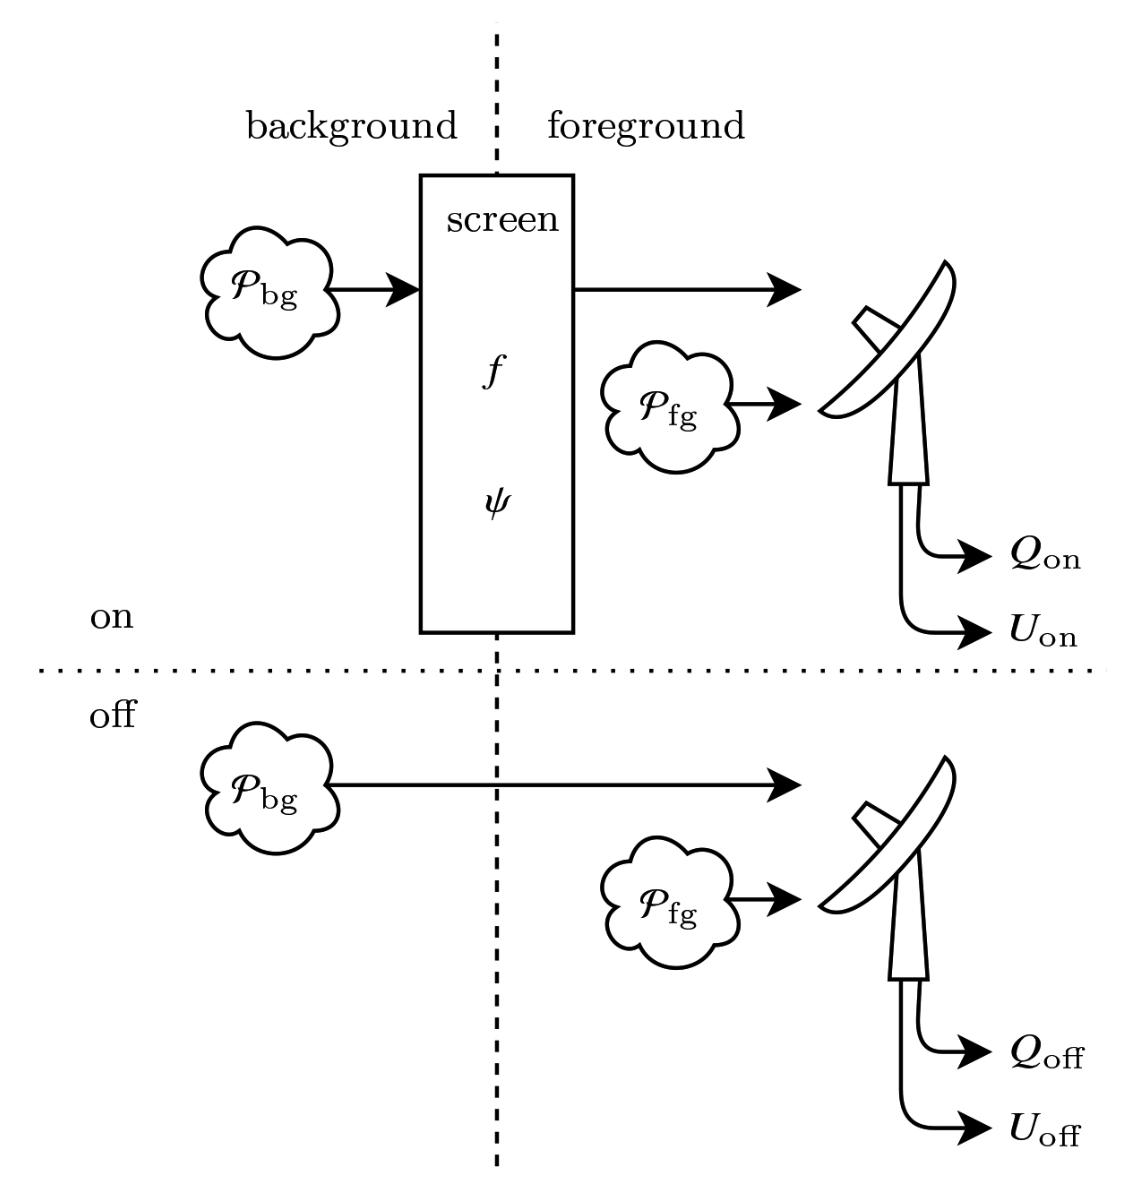
\includegraphics[width=8cm]{figures/FaradayScreenModel.png}}
\end{figure}

{\noindent}\textbf{Faraday thick:} A source is Faraday thick if the wavelength squared times the extent of the object in units of Faraday depth is much greater than 1: $\lambda^2\Delta\phi\gg1$. In the case of Faraday thick, objects are extended in Faraday space and substantially depolarized at wavelength squared. Remember that whether an object is Faraday thin or Faraday thick is wavelength dependent.

{\noindent}\textbf{Faraday thin:} A source is Faraday thin if the wavelength squared times the extent of the object in units of Faraday depth is much less than 1: $\lambda^2\Delta\phi\ll1$. In the case of Faraday thin, objects are well approximated by a Dirac-delta function in Faraday space. Remember that whether an object is Faraday thin or Faraday thick is wavelength dependent.

{\noindent}\textbf{Filling factor:} See \textit{volume filling factor}.

{\noindent}\textbf{First moment:} See \textit{mean}.

{\noindent}\textbf{Fluid turbulence:}

{\noindent}\textbf{Flux freezing:} The coupling between the \textit{cold neutral medium} (CNM) and the magnetic field due to its non-zero ionization fraction.

{\noindent}\textbf{Forbidden line:} Also known as a \textit{forbidden mechanism} or a \textit{forbidden transition}. A spectral line associated with the emission or absorption of light by atomic nuclei, atoms, or molecules which undergo a transition that is not allowed by a particular selection rule but does occur if the approximation associated with that rule is not made. Forbidden emission lines have been observed in extremely low-density gas and plasma in which collisions are infrequent. Under such conditions, once an atom or molecule has been excited for any reason into a meta-stable state, it is almost certain to decay by emission of a forbidden-line photon. Since meta-stable states are rather common, forbidden transitions account for a significant percentage of the photons emitted by the ultra-low density gas in space.

{\noindent}\textbf{Fourier transform ($\hat{f}(x)$):} Decomposes a function of time (a signal) into the frequencies that make it up. The Fourier transform (FT) of a function $f(x)$ is given by

\begin{align*}
    \hat{f}(x) = \int\limits_{-\infty}^\infty f(x')e^{-2\pi ixx'}dx'.
\end{align*}

{\noindent}The reason for the negative sign convention in the definition of $\hat{f}(x)$ is that the integral produces the amplitude and phase of the function $f(x')e^{-2\pi xx'}$ at frequency zero ($0$), which is identical to the amplitude and phase of the function $f(x')$ at frequency $x'$ , which is what $\hat{f}(x)$ is supposed to represent. The function $f(x)$ can be reconstructed from its Fourier transform $\hat{f}(x)$, which is known as the Fourier inverse theorem.

{\noindent}\textbf{Fourth moment:} See \textit{kurtosis}.

{\noindent}\textbf{Fractional polarization $(p(\alpha))$:}

{\noindent}\textbf{Galactic magnetic field (GMF):} Often the GMF is expressed in cylindrical coordinates ($\theta, r, z$). The \textit{azimuthal magnetic field} ($\vec{B}_\theta$) dominates the Galactic disk where the radial ($\vec{B}_r$) and vertical ($\vec{B}_z$) components are generally weak. The \textit{toroidal magnetic field} refers to the structures (without $\vec{B}_z$ components) confined to a plane parallel to the Galactic plane, while the \textit{poloidal magnetic field} refers to the axisymmetric field structure around $z$ (without $\vec{B}_\theta$ components) such as dipole fields. These terms are artificially designed for convenience when studying magnetic fields. Real magnetic fields would be all connected in space, with all components everywhere.

{\noindent}The RM sky is dominated by the GMF, with negligible contributions from the intergalactic medium and the RM intrinsic to the radio source (whether it be extragalactic radio sources or pulsars). A prominent feature of the RM sky is the antisymmetry in the inner Galactic quadrants ($|\ell|<90^\circ$). The positive RMs in the regions of ($0^\circ<\ell<90^\circ, b>0^\circ$) and ($270^\circ<\ell<360^\circ, b<0^\circ$) indicate that the magnetic fields point away from us. Such a high symmetry to the Galactic plane as the Galactic meridian through the Galactic center cannot simply be caused by localized features as previously thought. The antisymmetric pattern is very consistent with the magnetic field configuration of an $A0$ dynamo, which provides such toroidal fields with reversed directions above and below the Galactic plane. The toroidal fields possibly extend to the inner Galaxy, even towards the \textit{central molecular zone} (CMZ). This magnetic field model is also supported by the non-thermal radio filaments observed in the Galactic center region for a long time, which have been thought to be indications for the poloidal field in dipole form. The antisymmetric RM sky is also shown by pulsar RMs at high Galactic latitudes ($|b|>8^\circ$). This implies that the magnetic field responsible for the antisymmetry pattern could be nearer than the pulsars. 

{\noindent}\textbf{Generalized Faraday rotation:} In a medium whose natural modes are linearly or elliptically polarized, the counterpart of Faraday rotation, referred to as ``generalized Faraday rotation'', can lead to a partial conversion of linear into circular polarization.

{\noindent}\textbf{Great circle:} A circle on the surface of a sphere that lies in a plane passing through the sphere's center which represents the shortest distance between any two points on the surface of a sphere.

{\noindent}\textbf{Gyration frequency ($\omega$):} The angular frequency of circular motion.

{\noindent}\textbf{Hot ionized medium (HIM):} Diffuse interstellar gas with a typical temperature of $T\sim10^5-10^6\,{\rm K}$. This hot interstellar gas is believed to have been generated mainly by \textit{supernovae} and stellar winds from massive stars, forming as the shock wave sweeps through the \textit{interstellar medium}.

{\noindent}\textbf{Hydrogen spectral series:} Six named Hydrogen line series describing the emission spectrum of Hydrogen as dictated by the Rydberg equation. Includes the Lyman series ($n'=1$), Balmer series ($n'=2$), Paschen (or Bohr) series ($n'=3$), Brackett series ($n'=4$), Pfund series ($n'=5$), Humphreys series ($n'=6$).

{\noindent}\textbf{HI fibers:} Clark et al. (2014, 2015) identified slender, linear HI features called ``fibers'' in the Galactic Arecibo L-Band Feed Array HI (GALFA-HI) survey data. By developing a new machine vision transformation technique named the \textit{Rolling Hough Transform} (RHT), they identified the fibers and found that they are oriented along the interstellar magnetic fields probed by both starlight  and dust polarization. They also showed that angular dispersion of the fibers can be used to measure the magnetic field strength through the \textit{Chandrasekhar-Fermi method}. Based on the observed properties such as column density and line width, the HI fibers are suggested to be the CNM with density $\sim10\,{\rm cm^{-3}}$, temperature $\sim200\,{\rm K}$, and width $\sim0.1\,{\rm pc}$ and are embedded in a shell of the local bubble. From the theoretical point of view, neither the origin of the HI fibers nor the mechanism of the alignment of the fibers and magnetic field is yet understood.

{\noindent}t is known that when gas condensation is triggered by the thermal instability from a static thermally unstable medium, a CNM is formed that is flattened perpendicular to the magnetic field because magnetic pressure prevents the gas condensation except in the direction along the local magnetic field. Using three-dimensional MHD simulations, Inoue \& Inutsuka (2016) showed that shock sweeping of the magnetized WNM via supernova explosions creates thermally unstable gas in which fragmented HI clouds are formed as a consequence of the thermal instability. First, the shock compression creates a thermally unstable gas slab in which magnetic pressure balances upstream ram pressure. Then, the thermal instability develops to create the CNM in a cooling timescale of $\sim1\,{\rm Myr}$. Because the timescale of the thermal instability that enhances gas density is governed by the cooling timescale, the thermal pressure is decreased down to the initial upstream level by the time of the CMN formation. This leads to the formation of a CNM with density $n\lesssim100\,{\rm cm^{-3}}$. The CMN is formed via the thermal instability that drives runaway gas condensation along the local magnetic field. This is why the CNM clumps basically have a flattened shape. If the initial magnetic field is in the same direction as the shock propagation, or if the magnetic field is neglected, the CNM forms at much higher densities.

{\noindent}\textbf{HI shell/bubble:} HI shells, bubbles, supershells, and \textit{superbubbles} are large structures in the \textit{interstellar medium} (ISM) blown out by hot OB star clusters and supernovae. Both a \textit{supernova} and the winds from a massive star in its main sequence lifetime will each inject around $10^{51}-10^{53}\,{\rm ergs}$ into the ISM. These winds and shocks ionize what will become the cavity of the shell, and sweep out the neutral material. It is now understood that these objects are strongly influenced by magnetic fields in their formation. Magnetic fields both oppose the expansion of the shell from the exterior, and prevent the collapse of the swept up shell walls. HI shells have been discovered throughout our Galaxy as well as external galaxies. These objects play a large role in determining the dynamics, evolution, and overall structure of the ISM. Supershells and \textit{superbubbles} are the largest classification of HI shells, with radii between $10^2$ and $10^3\,{\rm pc}$.

{\noindent}\textbf{H$_\mathrm{II}$ region:} The ionized clouds around massive OB stars which are responsible for ionizing most of the hydrogen around such stars. The boundaries of H$_\mathrm{II}$ regions are determined by the volume in which the rate of UV photoionization equals the rate of recombination of electrons. When free electrons within an H$_\mathrm{II}$ region pass near a positive ion (H$^+$, He$^+$) they are accelerated by the Coulomb field and emit radiation known as ``free-free'' or \textit{bremsstrahlung emission} which is a source of polarized continuum emission. The average electron density of an H$_\mathrm{II}$ region is $\sim10^3\,{\rm cm^{-3}}$.

{\noindent}\textbf{Ideal magnetohydrodynamics (MHD):} Ideal MHD implies that fluid particles are attached to their field lines, that is to say they can flow along the field lines but cannot go across them. In a turbulent fluid, given the stochastic nature of the motions, such a situation would lead to a field that would be so tangled, that motions would quickly become prohibited. This implies that ideal MHD cannot, strictly speaking, be correct for a turbulent fluid and that some reconnection (i.e., some changes of the field lines topology) must be occurring. The physical origin of this reconnection is still debated but an appealing model has been proposed by Lazarian \& Vishniac (1999). In this view the reconnection is driven by turbulence and is a multi-scale process, that is unrelated to the details of the microphysical processes. It is certainly the case, at least in numerical simulations of MHD turbulence, where the numerical diffusivity is often controlling the reconnection, that the MHD is far to be ideal. This process in particular induces an effective diffusion of the magnetic flux, that is therefore not not fully frozen as one would expect if MHD was truly ideal.

{\noindent}\textbf{Incompressible turbulence:} The \textit{Kolmogorov power spectrum} for incompressible turbulence in three dimensions is $P(k)\propto k^{-11/3}$ while its \textit{energy spectrum} is $E(k)\propto k^{-5/3}$. In two dimensions, $P(k)\propto k^{-8/3}$ and $E(k)\propto k^{-5/3}$ (unchanged). For one dimension, $P(k)\propto k^{-5/3}$ and $E(k)\propto k^{-5/3}$ (unchanged).

{\noindent}\textbf{Induction equation:} Assuming a two-fluid description of a plasma with massless electrons, the magnetic field evolution is given by the generalized induction equation

\begin{align*}
    \frac{\partial\vec{B}}{\partial t} = \nabla\times(\vec{v}\times\vec{B}) + \frac{\eta c^2}{4\pi}\nabla^2\vec{B} - \frac{1}{en}\nabla\times(\vec{j}\times\vec{B}) - \frac{c}{ne}\nabla n\times\nabla T_e,
\end{align*}

{\noindent}which shows the evolution of magnetic field $\vec{B}$, based on the fluid velocity $\vec{v}$, the current density $\vec{j}=c\nabla\times\vec{B}/4\pi$, the number density $n$, and the electron temperature $T_e=P_e/n$, where $P_e$ is the electron plasma pressure. Here, $c$ is the speed of light, $\eta$ is the resistivity, and $e$ is the charge of an electron. The terms on the RHS from left to right are the convective term, the resistive term, the Hall term, and the Biermann battery term. The induction equation is often simplified by assuming that the system size $L$ is large compared to all kinetic scales, and only considering the convective term on the RHS. 

{\noindent}\textbf{Infrared polarization:} The same large-scale alignment of aspherical, spinning dust grains that causes \textit{starlight polarization} also causes polarization of far-infrared emission.

{\noindent}\textbf{Intensity of thermal dust emission ($I_\nu$)}: The intensity of the thermal dust emission, when optically thin, is given by

\begin{align*}
    I_\nu &= \tau_\nu B_\nu(T) ~ [{\rm W\,m^{-2}\,Hz^{-1}\,sr^{-1}}] \\
             &\equiv \sigma_e(\nu)N_{\rm H}B_\nu(T) ~ [{\rm W\,m^{-2}\,Hz^{-1}\,sr^{-1}}] \\
             &= r\mu m_{\rm H}N_{\rm H}\kappa_\nu B_\nu(T) ~ [{\rm W\,m^{-2}\,Hz^{-1}\,sr^{-1}}],
\end{align*}

{\noindent}where $\tau_\nu$ is the dust optical depth at frequency $\nu$, $B_\nu(T)$ is the Planck function, $\sigma_e(\nu)$ is the emission cross section per H nucleon (or ``opacity''), $N_{\rm H}$ is the total hydrogen column density (H in any form), $r$ is the dust-to-gas mass ratio, $\mu$ is the mean molecular weight of the gas, $m_{\rm H}$ is the hydrogen mass, and $\kappa_\nu$ is the dust mass (or emission) coefficient (or ``opacity'').

{\noindent}\textbf{Intergalactic medium (IGM):} 

{\noindent}\textbf{Internal depolarization:} Depolarization due to the spatial extent of the source and occurs even if the intervening media are completely homogenous. Along the line of sight, the emission from individual electrons within a source arrive from different depths and suffer different Faraday rotation angles due to different path lengths. For the total radiation emitted by a source, this results in a reduction of the observed degree of polarization.

{\noindent}\textbf{Interstellar medium (ISM):} A tenuous medium throughout galaxies that consists of three basic constituents: (1) ordinary matter, (2) relativistic charged particles called cosmic rays, and (3) magnetic fields. These three basic constituents have comparable pressures and are bound together by electromagnetic forces. The ordinary matter itself consists of gas (atoms, molecules, ions, and electrons) and dust (tiny solid particles) which can exist in a number of phases: molecular, cold atomic, warm atomic, warm ionized, and hot ionized. Apart from the densest parts of molecular clouds whose degree of ionization is exceedingly low, virtually all interstellar regions are sufficiently ionized for their neutral component to remain tightly coupled to the charged component and hence to the local magnetic field. Cosmic rays and magnetic fields influence both the dynamics of the ordinary matter and its spatial distribution at all scales, providing, in particular, an efficient support mechanism against gravity. Conversely, the weight of the ordinary (i.e., baryonic) matter confines magnetic fields and, hence, cosmic rays to the Galaxy, while its turbulent motion can be held responsible for the amplification of magnetic fields and for the acceleration of cosmic rays. Studies of the diffuse ($n\sim0.1-100\,{\rm cm^{-3}}$) HI suggests that the magnetic field strength is relatively independent of its volume density, in contrast to magnetic fields in molecular clouds. The Galactic origin of the most energetic cosmic rays and their widespread distribution throughout the Milky Way was not recognized until the observed Galactic radio emission was correctly identified with \textit{synchrotron radiation} emitted by cosmic-ray electrons gyrating about the local Galactic magnetic field. The ISM encloses but a small fraction of the total mass of the Galaxy. Moreover, it does not shine in the sky as visibly as stars do, yet it plays a vital role in many of the physical and chemical processes taking place in the Galactic ecosystem. The ISM is not merely a passive substrate within which stars evolve; it constitutes their direct partner in the Galactic ecosystem, continually exchanging matter and energy with them and controlling many of their properties. It is the spatial distribution of the ISM together with its thermal and chemical characteristics that determines where new stars form as well as their mass and luminosity spectra. These in turn govern the overall structure, optical appearance, and large-scale dynamics of our Galaxy. Hence understanding the present-day properties of our Galaxy and being able to predict its long-term evolution requires a good knowledge of the dynamics, energetics, and chemistry of the ISM. Table \ref{table:ismphases} outlines the different phases of the interstellar gas, including their typical temperature, number density, mass density, and total mass.

{\noindent}The MW is not a closed system. The evolution of the MW is significantly impacted by the two-way flow of gas and energy between the Galactic disk, halo, and IGM. We have long known that the atomic hydrogen halo extends far beyond the disk of the Galaxy. In recent years we have come to realize that the halo is also a highly structured and dynamic component of the Galaxy. Although we can now detect hundreds of clumped clouds in the atomic medium of the halo, we are far from understanding the halo's origin and its interaction with the disk of the Galaxy. It seems that a significant fraction of the structure of gas in the Galactic halo may be attributed to the outflow of structures formed in the disk, but extending into the halo. An example of such a structure may be an HI supershell. There are several examples of HI supershells that have grown large enough to effectively outgrow the Galactic HI disk. When this happens, the rapidly decreasing density of the Galactic halo does not provide sufficient resistance to the shell's expansion and it will expand unimpeded into the Galactic halo, creating a chimney from disk to halo. These chimneys supply hot, metal-enriched gas to the Galactic halo and may act as a mechanism for spreading metals across the disk. It has been theorized that HI chimneys in the disk of the Galaxy may be a dominant source of structure for the halo through a Galactic Fountain model. Some Fountain models predict that cold cloudlets should develop out of the hot gas expelled by chimneys on timescales of tens of millions of years. Other Fountain theories suggest that the cool caps of an HI supershell will extend to large heights above the Galactic plane before they break. Once broken, the remains of the shell caps could be an alternate source of small clouds for the lower halo. Recent observational work has placed this theory on firmer footing, showing that the clumped clouds that populate the lower halo are not only more prevalent in regions of the Galaxy showing massive star formation than in less active regions, but that they extend higher into the halo in these regions. 

\begin{table}[h]
\begin{center}
\captionof{table}{\footnotesize{Descriptive parameters of the different components of the interstellar gas. $T$ is the temperature, $n$ is the true (as opposed to space-averaged) number density of hydrogen nuclei near the Sun, $\Sigma_\odot$ is the azimuthally averaged mass density per unit area at the solar circle, and $\mathcal{M}$ is the mass contained in the entire Milky Way. Both $\Sigma_\odot$ and $\mathcal{M}$ include 70.4\% hydrogen, 28.1\% helium, and 1.5\% heavier elements. All values were rescaled to $R_\odot=8.5\,{\rm kpc}$ Table taken from Ferri\'ere (2001).}} \label{table:ismphases}
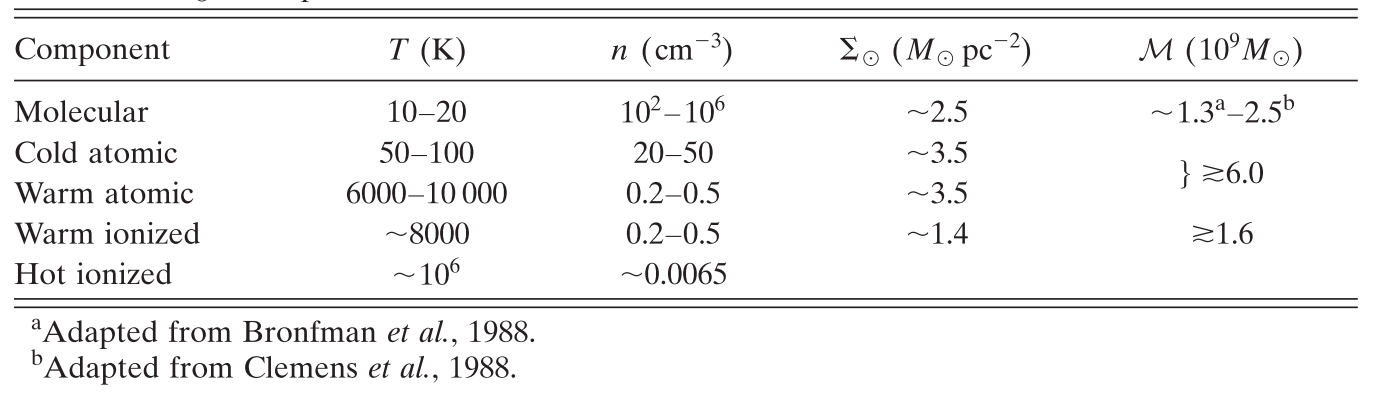
\includegraphics[width=15cm]{figures/ISMphases.png}
\end{center}
\end{table}

{\noindent}\textbf{Inverse Compton scattering:} The up-scattering of radio photons to become optical or X-ray photons by means of the inelastic scattering of a charged particle (usually an electron).

{\noindent}\textbf{Inverse Fourier transform (IFT):} The reconstruction of a function from its decomposition into the frequencies that make it up. The inverse Fourier transform (IFT) is given by

\begin{align*}
    f(x) = \int\limits_{-\infty}^\infty \hat{f}(x')e^{2\pi ixx'}dx'.
\end{align*}

{\noindent}The fact that a function $f(x)$ can be reconstructed from its Fourier transform $\hat{f}(x)$ is known as the Fourier inverse theorem.

{\noindent}\textbf{Ion-neutral drift:} See \textit{ambipolar diffusion}.

{\noindent}\textbf{Ion-neutral friction:} See \textit{ambipolar diffusion}.

{\noindent}\textbf{Kelvin-Helmholtz instability:}

{\noindent}\textbf{Kolmogorov microscale:}

{\noindent}\textbf{Kolmogorov spectrum:}

{\noindent}\textbf{Kurtosis ($\beta_x$):} The fourth order statistical \textit{moment} which is a measure of whether the data are heavy-tailed or light-tailed relative to a normal distribution. That is, data sets with high kurtosis tend to have heavy tails, or outliers. Data sets with low kurtosis tend to have light tails, or lack of outliers. Kurtosis is defined as

\begin{align*}
    \beta_x = \frac{1}{N} \sum_{i=1}^N \left(\frac{x_i-\mu_x}{\sigma}\right)^3 ~ [{\rm dimensionless}],
\end{align*}

{\noindent}where $\mu_x$ is the statistical mean and $\sigma$ is the standard deviation. Like the \textit{skewness}, it is a dimensionless quantity.

{\noindent}\textbf{Large scale magnetic field:} How large is the ``large'' scale? Obviously it should be a scale, relatively much larger than some kind of standard. For example, the large-scale magnetic field of the Sun refers to the global scale field or the field with a scale length comparable to the size of the Sun, up to $10^9\,{\rm m}$, rather than small-scale magnetic fields on the Solar surface. For the magnetic fields of our Galaxy, we should define the ``large'' scale as being a \textit{scale larger than the separation between spiral arms}. That is to say, large scale means a scale larger than $2-3\,{\rm kpc}$. Note that in the literature, ``large'' scale is sometimes used for large angular scale when discussing the structures or prominent plane-of-the-sky features (e.g., the large-scale features in radio continuum surveys). These large angular scale features are often very localized phenomena, and not very large in linear scale.

{\noindent}\textbf{Lorentz factor ($\gamma$):} The factor by which time, length, and relativistic mass change for an object while that object is moving with speed $\mathbf{v}$:

\begin{align*}
    \gamma = \sqrt{\frac{1-(v/c)^2}{c^2}}.
\end{align*}

{\noindent}For non-relativistic motion $\gamma\approx1$, while for relativistic motion $\gamma>1$. For example, $\gamma(v=0.9c)\approx2$ and $\gamma(v=0.99c)\approx7$.

{\noindent}\textbf{Lorentz force:} The combination of electric and magnetic force on a point charge due to electromagnetic fields. A particle of mass $m$ and charge $q$ moving with a velocity $v$ within a magnetic field $\mathbf{B}$ experiences a force 

\begin{align*}
    \vec{F} = \dfrac{\mathrm{d}}{\mathrm{d}\tau} (m\gamma\vec{v}) = q\left(\vec{E} + \dfrac{\vec{v}}{c}\times\vec{B}\right) ~ [{\rm N}],
\end{align*}

{\noindent}where $\tau$ is the retarded time and $\gamma$ is the Lorentz factor. Of course, the Lorentz force only acts on charged particles but its effect is then transmitted to neutral particles via ion-neutral collisions.

{\noindent}\textbf{Luminosity per H atom ($L$):} A key quantity is the luminosity per H atom emitted by dust grains (equal to the absorbed power) computed by integrating the SED over $\nu$:

\begin{align*}
    L = \int 4\pi\kappa_0(\nu/\nu_0)^\beta \mu m_{\rm H}B_\nu(T) \,{\rm d}\nu ~ [{\rm W\,H^{-1}}].
\end{align*}

{\noindent}\textbf{Mach number ($\mathcal{M}$):}

{\noindent}\textbf{Magnetic buoyancy:} See Rayleigh-Taylor instability.

{\noindent}\textbf{Magnetic reconnection:}

{\noindent}\textbf{Magnetohydrodynamic (MHD) equations:} The equations of ideal MHD assume that the fluids are perfect conductors. The Lorentz force, which is the force that the EM fields $\vec{E}$ and $\vec{B}$ exert on the fluid must be taken into account. The EM field evolution is described by Maxwell equations. Written in CGS units, these equations are

\begin{align*}
    \vec\nabla\cdot\vec{B} &= 0 \\
    \vec\nabla\cdot\vec{E} &= 4\pi\rho_e \\
    c\vec\nabla\times\vec{E} &= - \frac{\partial\vec{B}}{\partial t} \\
    c\vec\nabla\times\vec{B} &= 4\pi\vec{j} + \frac{\partial\vec{E}}{\partial t},
\end{align*}

{\noindent}where $\rho_e$ and $\vec{j}$ are the fluid charge and current densities. The equation for charge conservation links these two quantities:

\begin{align*}
    \frac{\partial\rho_e}{\partial t} + \vec\nabla\cdot\vec{j} = 0.
\end{align*}

{\noindent}\textbf{Magnetohydrodynamics (MHD):} Magnetohydrodynamics (MHD) denotes the study of the dynamics of electrically conducting fluids. It establishes a coupling between the \textit{Navier-Stokes equations} for fluid dynamics and Maxwell's equations for electromagnetism. The main concept behind MHD is that magnetic fields can induce currents in a moving conductive fluid, which in turn create forces on the fluid and influence the magnetic field itself. 

{\noindent}\textbf{Magnetoionic medium (MIM):}

{\noindent}\textbf{Magnetorotational instability:} See Balbus-Hawley instability.

{\noindent}\textbf{Mass absorption coefficient ($\kappa_\nu$):} Also called the ``opacity'' of the interstellar material:

\begin{align*}
    \kappa_\nu = \kappa_0 \left(\frac{\nu}{\nu_0}\right)^\beta ~ [{\rm cm^2\,g^{-1}}].
\end{align*}

{\noindent}It is related to the mass emission cross section per H nucleon via

\begin{align*}
    \kappa_\nu = \frac{\sigma_e(\nu)}{\mu m_{\rm H}} ~ [{\rm cm^2\,g^{-1}}].
\end{align*}

\begin{align*}
    \kappa_\nu = \kappa_0 \left(\frac{\nu}{\nu_0}\right)^\beta ~ [{\rm cm^2\,g^{-1}}]
\end{align*}

{\noindent}\textbf{Mean ($\mu_x$):} The first order statistical \textit{moment} which is a measure of the central tendency. The mean is defined as

\begin{align*}
    \mu_x = \frac{1}{N} \sum_{i=1}^N x_i
\end{align*}

{\noindent}and has the same dimensions as $x_i$.

{\noindent}\textbf{Mean molecular weight ($\mu$):}

{\noindent}\textbf{Meridian:} A circle of constant longitude passing through a given place on Earth's surface and the terrestrial poles.

{\noindent}\textbf{Microturbulence:}

{\noindent}\textbf{Milky Way Galaxy (MWG):} We see the Milky Way as a narrow band encircling us because the Galaxy has the shape of a flattened disk within which we are deeply embedded. Our Galaxy comprises a thin disk with radius $\sim25-30\,{\rm kpc}$ and effective thickness $\sim400-600\,{\rm pc}$, plus a spherical system itself composed of a bulge with radius $\sim2-3\,{\rm kpc}$ and a halo extending out to more than $30\,{\rm kpc}$ from the center. The Sun resides in the Galactic disk, approximately $15\,{\rm pc}$ from the midplane and $8.5\,{\rm kpc}$ away from the center. The stars belonging to the disk rotate around the Galactic center in nearly circular orbits. Their angular rotation rate is a decreasing function of their radial distance. At the Sun's orbital distance, the Galactic rotation velocity is $\simeq220\,{\rm km\,s^{-1}}$, corresponding to a rotational period of $\simeq240\times10^6\,{\rm years}$. Disk stars also have a velocity dispersion of $\sim10-40\,{\rm km\,s^{-1}}$ which causes them to experience small oscillations about a perfectly circular orbit both in the Galactic plane (epicycles) and the vertical direction. In contrast, stars in the bulge and the halo rotate slowly and often have very eccentric orbits. Radio observations of interstellar neutral hydrogen indicate that the Milky Way possesses a spiral structure similar to those seen in optical wavelengths of external galaxies. The exact spiral structure of our own Galaxy is difficult to determine from within; the best radio data to date points to a structure characterized by a bulge of intermediate size and a moderate winding of the spiral arms. Infrared (IR) images of the Galactic center clearly display the distinctive signature of a bar. Our position in the spiral pattern can be derived from local optical measurements which give quite an accurate outline of the three closest arms; they locate the Sun between the inner Sagittarius arm and the outer Perseus arm, near the inner edge of the local Orion-Cygnus arm.

{\noindent}\textbf{Modified blackbody ($I_\nu$):} The dust emission process is thermal, with dust grains emitting a modified blackbody spectrum following:

\begin{align*}
    I_\nu = \tau B_\nu(T) \left(\frac{\nu}{\nu_0}\right)^\beta ~ [{\rm W\,m^{-2}\,Hz^{-1}\,sr^{-1}}],
\end{align*}

{\noindent}where $B_\nu(T)$ is the \textit{Planck function}, and $\tau$ is the dust \textit{optical depth}. Grains of interstellar dust, distributed throughout the ISM of a galaxy, are heated to temperatures between about $20$ and $200\,{\rm K}$, depending on the spectrum and intensity of the \textit{interstellar radiation field} (ISRF), and the size and optical properties of the grains. Higher dust temperatures can be produced close to a powerful source of radiation, with dust subliming at temperatures of order $2000\,{\rm K}$. Very small grains can be heated far above their equilibrium temperatures by absorbing hard-UV photons. Lower dust temperatures, always exceeding the CMB temperature, are possible in opaque regions of the ISM that are shielded from intense heating, in the intergalactic medium or in regions with an intrinsically weak ISRF.

{\noindent}The minimum parameters necessary to describe the emission from dust grains are a temperature $T$ and a form of the emissivity function $\epsilon_\nu$. In any galaxy there will be a distribution of dust temperatures, reflecting the different nature and environment of each grain. It is useful to use $T$ to describe the coolest grains that contribute significantly to the energy output of a galaxy when discussing submm observations. In most cases, spatially and spectrally resolved images of galaxies are not available, and so it is reasonable to assume a volume-averaged description of the emissivity function as a function of frequency $\nu$, $\epsilon_\nu\propto\nu^\beta$. Values of $\beta$ in the range $1-2$ are usually assumed. Scattering theory predicts that  $\beta\sim2$ at low frequencies, while a value $\beta\sim1$ at high frequencies matches the general trend of the interstellar extinction curve that describes the properties of absorption of optical and UV radiation by the ISM. The simplest form of the emission spectrum/SED, $I_\nu$ is given by assuming that $I_\nu\propto\epsilon_\nu B_\nu$, in which $B_\nu$ is the \textit{Planck function} ($2kT\nu^2/c^2$ in the \textit{Rayleigh-Jeans limit}, in units of $\rm W\,m^{-2}\,Hz^{-1}\,sr^{-1}$). This assumes that the emitting source is optically thin. 

{\noindent}\textbf{Molecular medium (MM):} Molecular gas is explored primarily with the $2.6\,{\rm mm}$ and other radio emission lines of the second most abundant molecule, CO, and secondarily with radio emission and absorption lines of less abundant molecules, such as OH, H$_2$O, and NH$_3$. Historically, molecular lines were seen mainly in emission towards the standard dense molecular clouds, and CO was emphasized to the extent that its presence \textit{defined} molecular gas. While Spatially, the molecular gas is confined to discrete clouds, which are roundish, gravitationally bound, and organized hierarchically from large complexes (size $\sim20-80\,{\rm pc}$ and mass $\sim10^5-10^6\,{\rm M_\odot}$) down to small clumps (size $\lesssim0.5\,{\rm pc}$, mass $\lesssim10^3\,{\rm M_\odot}$). Along the vertical direction, the molecular gas is the most strongly confined to the Galactic plane, with a HWHM thickness near the Sun $\sim70-80\,{\rm pc}$. Horizontally, all the gas components tend to concentrate along the spiral arms, this tendency being probably most pronounced for the molecular gas. Upon averaging along Galactic circles, through spiral arms and interarm regions, it is found that most of the molecular gas resides in a ring extending radially between $3.5-7\,{\rm kpc}$ from the Galactic center. It seems almost certain that the DMM is a transition state between the CNM and classical MM. Moreover, we expect the details of the DMM transition region to depend not only on physical conditions but also cloud morphology as it determines whether UV photons can penetrate to destroy molecules via photodissociation or photoionization. It seems very unlikely that one can understand the transition between atomic and molecular gas without understanding the effect of UV photons, and thus cloud morphology. In addition, there are hints that cloud morphology is affected by the magnetic field; after all, magnetic forces are one of the important forces on the ISM (the others being turbulent pressure, cosmic ray pressure (coupled to the gas by the magnetic field), thermal pressure, and gravity).

{\noindent}\textbf{Neural network (NN):}A standard neural network is composed of neurons: a neuron takes in some inputs and provides an output

\begin{align*}
    y = f \left(\sum_{i=1}^dx_i\cdot w_i\right),
\end{align*}

{\noindent}where $x_i$ is the input vector, $w_i$ are a set of trainable weights, and $f$ is some non-linear, typically monotonically increasing, activation function. Common choices for the activation function are linear rectification $[f(x) = \max (x, 0)]$, which gives rise to rectified linear units, or a sigmoidal function $[f(x) = (1+e^{-x})-1$ or $f(x) = \tanh(x)]$. Another possibility is to compute the maximum across several linear combinations of the input, which gives rise to maxout units. In this way a network can be built up by connecting the outputs of many neurons on some layer $j$ to many neurons on the next layer $j+1$. In this way a network can be built up by connecting the outputs of many neurons on some layer $j$ to many neurons on the next layer $j+1$. A ``fully connected layer'' is a set of weights between layers of neurons that connects all neurons on level $j$ to level $j+1$. A network will typically narrow, until the number of final neurons is equal to the number of classes the network is being designed to distinguish. The process of training a network consists of providing labeled data to the network and measuring the resultant class. If the class is incorrect the weights are adjusted through back-propagation of error. In most modern training scenarios a small subset of the training data is presented to the network at a time, and the weights are adjusted in a process called stochastic gradient descent.

{\noindent}\textbf{$\mathbf{n\pi}$ ambiguity:} The inability to distinguish between polarization angles modulo $\pi$ radians, rendering traditional linear RM fits often arbitrary. One way to deal with this ambiguity is to rely on resolving smooth spatial gradients in the polarization angle at each wavelength. With this assumption, the appropriate value of $n$ can be resolved for each spatial pixel, yielding the correct polarization angle at each wavelength and thus the true value of RM. This is the basis of the PACERMAN routine developed by Dolag et al., (2005). However, routines like PACERMAN cannot deal with the second and third problems listed above since it is ultimately based on fitting a single value of RM along each line of sight. 

{\noindent}\textbf{Open cluster:} A rather loose, irregular grouping of $10^2-10^3$ stars confined to the Galactic disk and therefore also known as Galactic clusters. 

{\noindent}\textbf{Optical depth ($\tau_\nu$):} 

{\noindent}\textbf{Ordered magnetic field:} Also known as ``coherent magnetic field''. Whether a magnetic field is ordered or random depends on the scales concerned. A uniform field at a $1\,{\rm kpc}$ scale could be part of random fields on a $10\,{\rm kpc}$ scale, while it is of a very large scale relative to the $\rm pc$ scale magnetic fields in molecular clouds. Uniform fields are ordered fields. Regularly ordered fields can coherently change their directions, so they may not be uniform fields. 

{\noindent}\textbf{Paramagnetism:} Paramagnetic materials have unpaired electrons which, when in the presence of an external magnetic field such as the interstellar magnetic field, align in the same direction causing grain alignment.

{\noindent}\textbf{Parker instability:}

{\noindent}\textbf{Partially ionized plasma (PIP):} It is assumed that a PIP is composed of multiple kind of particles such as electrons, ions that can have different ionization states, neutral particles with zero ionization, as well as dust grains, positively or negatively charged. The concept of a fluid can be applied separately to each of these components in all the environments of interest. Therefore the behavior of such a plasma can be described by a set of equations of mass, momentum, and energy conservation for each of the components.

{\noindent}\textbf{Passive mixing:}

{\noindent}\textbf{Pitch angle:} The angle between a charged particle's velocity vector and the local magnetic field.

{\noindent}\textbf{Photodissociation region (PDR):} Also known as \textit{photon-dominated regions} or PDRs. Predominantly neutral regions of the ISM in which UV photons strongly influence the gas chemistry and act as the dominant energy source. They occur in any region of interstellar gas that is dense and cold enough to remain neutral, but that has too low of a column density to prevent penetration of far-UV photons from massive stars. They are also associated with HII regions. All of the atomic gas and most of the molecular gas is found in photodissociation regions.

{\noindent}\textbf{Photon-dominated region (PDR):} See \textit{photodissociation region}.

{\noindent}\textbf{Pitch angle:} The angle between a charged particle's velocity vector and the local magnetic field.

{\noindent}\textbf{Planck function ($B_\nu(T)~{\rm or}~B_\lambda(T)$):} The spectral radiance of an object at a given temperature as a function of frequency or wavelength:

\begin{align*}
    B_\nu(T) = \left(\frac{2h\nu^3}{c^2}\right) \frac{1}{e^{h\nu/k_BT}-1} ~ [{\rm W\,m^{-2}\,Hz^{-1}\,sr^{-1}}] \\
    B_\lambda(T) = \left(\frac{2hc^2}{\lambda^5}\right) \frac{1}{e^{hc/\lambda k_BT}-1} ~ [{\rm W\,m^{-2}\,m^{-1}\,sr^{-1}}].
\end{align*}

{\noindent}\textbf{Plasma beta ($\beta_{\rm th}$):} The ratio of the gas to magnetic pressure:

\begin{align*}
    \beta_{\rm th} = \frac{P_{\rm th}}{P_{\rm mag}} ~ [{\rm dimensionless}]
\end{align*}

{\noindent}and can also be defined as

\begin{align*}
    \beta_{\rm th} = \frac{2M_A^2}{M_S^2} ~ [{\rm dimensionless}],
\end{align*}

{\noindent}where $M_A$ and $M_S$ are the \textit{Alfv\'enic} and \textit{sonic} Mach numbers, respectively.

{\noindent}For a mixture of \textit{warm neutral medium} (WNM) and \textit{warm ionized medium} (WIM), this becomes

\begin{align*}
\beta_{\rm th} &= \frac{ \langle P_{\rm th,i}\rangle + \langle P_{\rm th,n}\rangle }{(B_{\rm tot}^2/8\pi)} ~ [{\rm dimensionless}] \\
                      &= \frac{2\langle n_e\rangle k_BT_i + \langle n_{\rm H}\rangle k_BT_n}{(B_{\rm tot}^2/8\pi)}  ~ [{\rm dimensionless}] \\
                      &= \frac{2f_en_e+ \langle n_{\rm H}\rangle k_BT_n}{(B_{\rm tot}^2/8\pi)}  ~ [{\rm dimensionless}],
\end{align*}

{\noindent}where $\langle P_{\rm th,i}\rangle$ and $\langle P_{\rm th,n}\rangle$ are the ionized and neutral thermal pressures, respectively.

{\noindent}This quantity is very important in plasma fluid dynamics. It gives the relative importance of the gas pressure to the magnetic field as the restoring force to any disturbance. If $\beta\gg1$, then the magnetic force has a negligible effect on the dynamics, but the magnetic field is still advected by the flow. This is called MHD kinematics. It is important in studies of the generation of a magnetic field by a conducting fluid undergoing motion forced by other means, such as convection in a gravitational field. The generation of a large-scale magnetic field by convective turbulence is called the dynamo effect, and it is thought to be the most likely scenario for the origin of planetary and stellar magnetic fields. In the opposite limit, $\beta\ll1$, the gas pressure drops out of the MHD force equation to lowest order in $\beta$, but it remains as a slight correction to the geometry of any equilibrium. For such a low-beta plasma, the gas pressure is still important because it can break the tendency of magnetic pressure and tension to cancel. A consequence is that a finite gas pressure prevents the establishment of a force-free equilibrium, to which the plasma tends to relax in many important configurations, even in a situation with a nonzero current density. In addition, the gas pressure can cause instability in an equilibrium which would otherwise be stable to MHD perturbations (MHD-stable).

{\noindent}For either high or low $\beta$, it was predicted that \textit{Alfv\'en waves} should should damp at the \textit{ambipolar diffusion scale} $L_\mathrm{AD}$ and thus the magnetohydrodynamic (MHD) cascade should damp past the ambipolar diffusion scale.

{\noindent}\textbf{Poincar\'e sphere:}

{\noindent}\textbf{Polarized intensity ($P$):} A measure of the total linear polarization in radio emission given as

\begin{align*}
    P\equiv\sqrt{Q^2+U^2} ~ [{\rm Jy}],
\end{align*}

{\noindent}where $Q$ is the \textit{Stokes Q} polarization and $U$ the \textit{Stokes U} polarization. The images of $P$ (as well as $Q$ and $U$) are often filled with complex structures that bear little resemblance to the \textit{Stokes I} image of total intensity. The intensity variations seen in $P$ (as well as $Q$ and $U$) are the result of small-scale angular structure in the \textit{Faraday rotation} induced by ionized gas, and are thus an indirect representation of turbulent fluctuations in the free-electron density and magnetic field throughout the \textit{interstellar medium}. while $Q$ and $U$ exhibit Gaussian noise properties, this is not true for $P$. The noise in $Q$ and $U$ is squared when calculating $P$, having a Ricean distribution, which causes the observed polarization intensity to be biased toward larger values.

{\noindent}In addition to the true polarized signal of a source $P_T$, root mean squared (rms) noise obtained from the receiving system is also detected. If we use the standard formula to calculate $\hat{P}$ from the measured data $\hat{U}$ and $\hat{Q}$ , $\hat{P}$ can be expressed by the polarized components of the source $U_T$ and $Q_T$ and their noise contributions $\sigma_U$ and $\sigma_Q$:

\begin{align*}
    \hat{P} &= \sqrt{\hat{Q}^2 + \hat{U}^2} ~ [{\rm Jy}] \\
                &= \sqrt{(Q_T+\sigma_Q)^2 + (U_T+\sigma_U)^2} ~ [{\rm Jy}].
\end{align*}

{\noindent}The noise always delivers a positive bias to the true polarized intensity $P_T$ that cannot be separated out for small signal-to-noise (S/N) ratios. The distribution of $\hat{P}$ is Ricean for small S/N and becomes Gaussian for large S/N. Several methods have been developed to correct for this noise bias. The most widely used method is that of Wardle \& Kronberg (1974) who proposed the following bias correction for $\hat{P}$ maps:

\begin{align*}
    P_T = \sqrt{\hat{P}^2 - \sigma^2} ~ [{\rm Jy}],
\end{align*}

{\noindent}where $\sigma$ is the rms standard deviation of the noise distributions in $\hat{U}$ and $\hat{Q}$.

{\noindent}A new method to suppress the bias in polarized intensity was proposed by M\"{u}ller et al. (2017).

{\noindent}\textbf{Polarization angle $(\chi)$:} Given by

\begin{align*}
    \chi\equiv\frac{1}{2}\arctan\left(\frac{U}{Q}\right) ~ [{\rm rad}],
\end{align*}

{\noindent}where $Q$ is the \textit{Stokes Q} polarization vector and $U$ the \textit{Stokes U} polarization vector. The arctan2 function is generally used to determine $\chi$ over the full $\pm n\pi$ range. The polarization angle (likewise with the amplitude of \textit{polarized intensity}) is not preserved under arbitrary rotations and translations of the \textit{Q-U plane}. In the most general case, then, the observed values of $\chi$ (and $\mathbf{P}\equiv\sqrt{Q^2+U^2}$) do not have any physical significance; only measurements of quantities that are both rotationally and translationally invariant in the $Q-U$ plane can provide insight into the physical conditions that produce the observed polarization distribution.

{\noindent}\textbf{Polarization fraction $(p(\lambda^2))$:}

\begin{align*}
    p(\lambda^2) = \frac{P(\lambda^2)}{I(\lambda^2)} ~ [{\rm dimensionless}],
\end{align*}

{\noindent}where $P(\lambda^2)$ is the polarized surface brightness and $I(\lambda^2)$ is the total surface brightness.

{\noindent}\textbf{Polarization gradient ($\lvert\vec{\nabla}\vec{P}\rvert$):} The rate at which the \textit{polarized intensity} complex vector $\vec{P}\equiv\sqrt{Q^2+U^2}$ traces out a trajectory in the \textit{Q-U} plane as a function of position on the sky given by

\begin{align*}
    \lvert\vec\nabla\vec{P}\rvert = \sqrt{\left(\frac{\partial Q}{\partial x}\right)^2 + \left(\frac{\partial U}{\partial x}\right)^2 + \left(\frac{\partial Q}{\partial y}\right)^2 + \left(\frac{\partial U}{\partial y}\right)^2} ~ [{\rm Jy\,beam^{-1}}],
\end{align*}

{\noindent}or

\begin{equation*}
\begin{split}
\left\lvert\dfrac{\partial\vec{P}}{\partial s}\right\rvert_\mathrm{max} = \sqrt{ \frac{1}{2}\left[ \left(\frac{\partial Q}{\partial x}\right)^2 + \left(\frac{\partial U}{\partial x}\right)^2 + \left(\frac{\partial U}{\partial x}\right)^2 + \left(\frac{\partial U}{\partial y}\right)^2 \right] + \frac{1}{2} 
  \sqrt{
    \begin{aligned}
    & \left[ \left(\frac{\partial Q}{\partial x}\right)^2 + \left(\frac{\partial U}{\partial x}\right)^2 + \left(\frac{\partial U}{\partial x}\right)^2 + \left(\frac{\partial U}{\partial y}\right)^2 \right]^2 \\
    &- 4\left[ \frac{\partial Q}{\partial x}\frac{\partial U}{\partial y} - \frac{\partial Q}{\partial y}\frac{\partial U}{\partial x}  \right]^2,
    \end{aligned}
    }}
\end{split}
\end{equation*}

{\noindent}where $Q$ and $U$ are the complex \textit{Stokes vectors} and $x$ and $y$ are the Cartesian axes of the image plane. Note that $\lvert\nabla\vec{P}\rvert$ cannot be constructed from the scalar quantity $P\equiv\sqrt{Q^2+U^2}$, but is derived from the vector field $\vec{P}\equiv(Q,U)$. The amplitude of the polarization gradient $\lvert\vec\nabla\vec{P}\rvert$ provides an image of magnetized turbulence in diffuse, ionized gas manifested as a complex filamentary web of discontinuities in gas density and magnetic field strength. This quantity is rotationally and translationally invariant in the $Q-U$ plane, and so has the potential to reveal properties of the polarized distribution that might otherwise be hidden by excess foreground emission or \textit{Faraday rotation}, or in data sets from which large-scale structure is missing. The polarization gradient is shown in Figure \ref{figure:delP}.

\begin{figure}[h]
\begin{center}
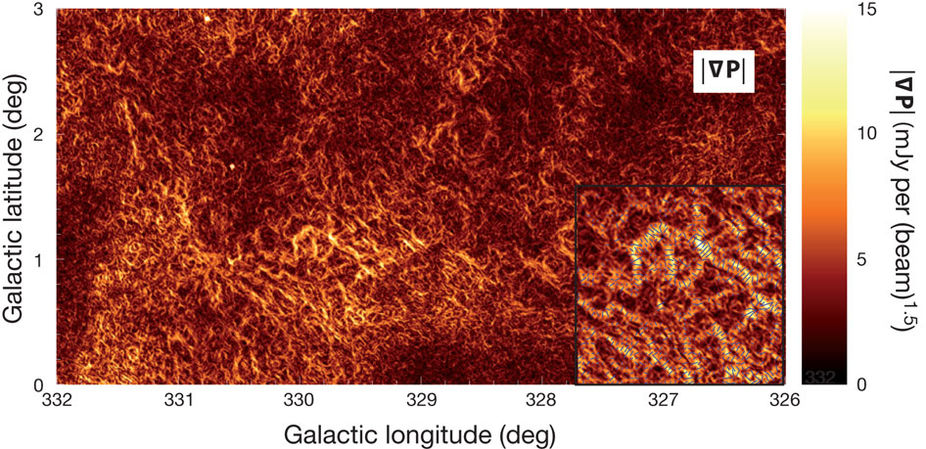
\includegraphics[width=12cm]{figures/delP.jpg}
\caption{\footnotesize{$\lvert\vec\nabla \vec{P}\rvert$ for an $18$-deg$^2$ region of the Southern Galactic Plane Survey which reveals a complex network of tangled filaments. In particular, all regions in which $\lvert\nabla \vec{P}\rvert$ is high consists of elongated, narrow structures rather than extended patches. In the inset, the direction of $\lvert\nabla\mathbf{P}\rvert$ is shown for a small subregion of the image, demonstrating that $\lvert\nabla\vec{P}\rvert$ changes most rapidly along directions oriented perpendicular to the filaments. Figure taken from Gaensler (2011).}}
\label{figure:delP}
\end{center}
\end{figure}

{\noindent}Using polarization gradients of isothermal MHD turbulence, the supersonic case (Figure \ref{figure:delPmach}c) was found to show localized groupings of very high-gradient filaments, corresponding to ensembles of intersecting shocks. By contrast, the subsonic (Figure \ref{figure:delPmach}a) and tran-sonic (Figure \ref{figure:delPmach}b) cases showed more diffuse networks of filaments, representing the cusps and discontinuities characteristic of any turbulent velocity field. 

\begin{figure}[h]
\begin{center}
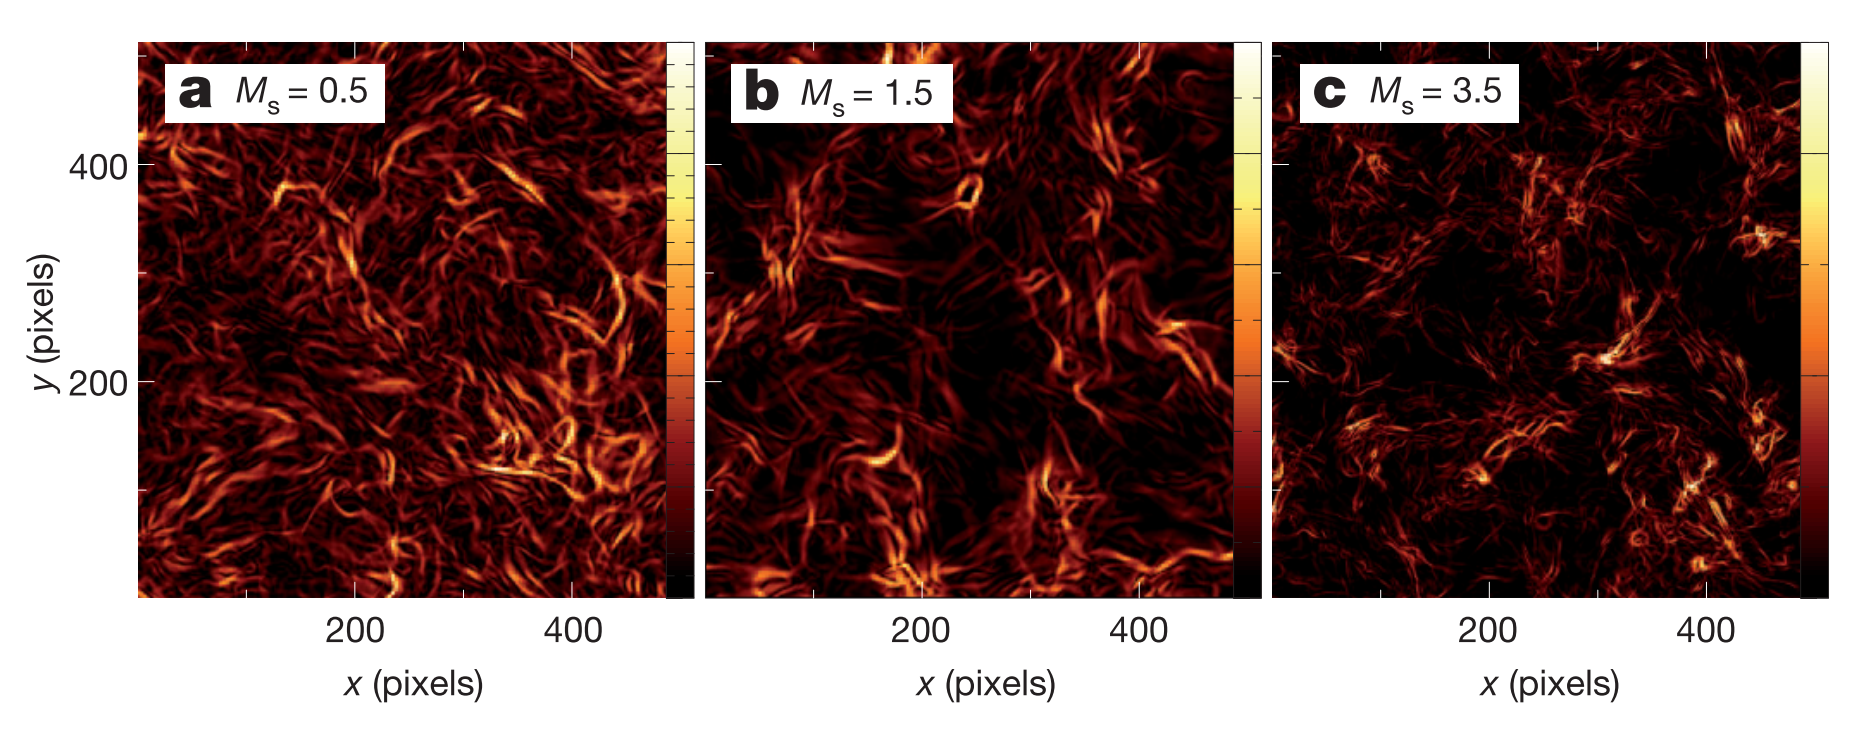
\includegraphics[width=12cm]{figures/delP_mach.png}
\caption{\footnotesize{$\lvert\vec\nabla \vec{P}\rvert$ derived from propagation of linear radio polarization through three different isothermal simulations of magnetized turbulence. Figure taken from Gaensler (2011).}}
\label{figure:delPmach}
\end{center}
\end{figure}

{\noindent}In the ISM, fluctuations in density and magnetic field will occur as a result of MHD turbulence, which will be visible in polarimetric maps. In the case of taking gradients of a turbulent field, one would expect to find filamentary structure created by shock fronts, jumps, and discontinuities. Figure \ref{fig:polgradprofiles} shows a schematic illustrating these three separate cases of a possible profile and its respective derivative. The cases are as follows:

\begin{itemize}
    \item A H\"older continuous profile that is not differentiable at a given point (e.g., the absolute value function at the origin): common for all types of MHD turbulence. It is known that the turbulent velocity field in a Kolmogorov-type inertial range both in hydro and MHD is not differentiable, but only H\"older continuous. This case can be found in both subsonic- and supersonic turbulence.
    \item A jump profile: weak shocks, strong fluctuations, or edges (e.g., a cloud in the foreground which suddenly stops). This case creates a structure in the gradient by a shock jump or a large fluctuation in either $n_e$ or $\vec{B}$. Here again, this type of enhancement in $\lvert\nabla\vec{P}\rvert$ could be found in supersonic- and subsonic turbulence, and is due either to large random spatial increases or decreases due to turbulent fluctuations along the LOS or weak shocks. We expect weak shock turbulence to show a larger amplitude in $\lvert\nabla\vec{P}\rvert$ than the subsonic case due to increases in density fluctuations.
    \item A spike profile (e.g., delta function): strong shock regime. This case is unique to supersonic turbulence in that it represents a very sharp spike in $n_e$ and/or $\vec{B}$ across a shock front. The difference between this case and what might be seen in case two is that here we are dealing with interactions of strong shock fronts, which are known to create delta function-like distributions in density, creating a ``double jump'' profile across the shock front.
\end{itemize}

\begin{figure}[h]
\begin{center}
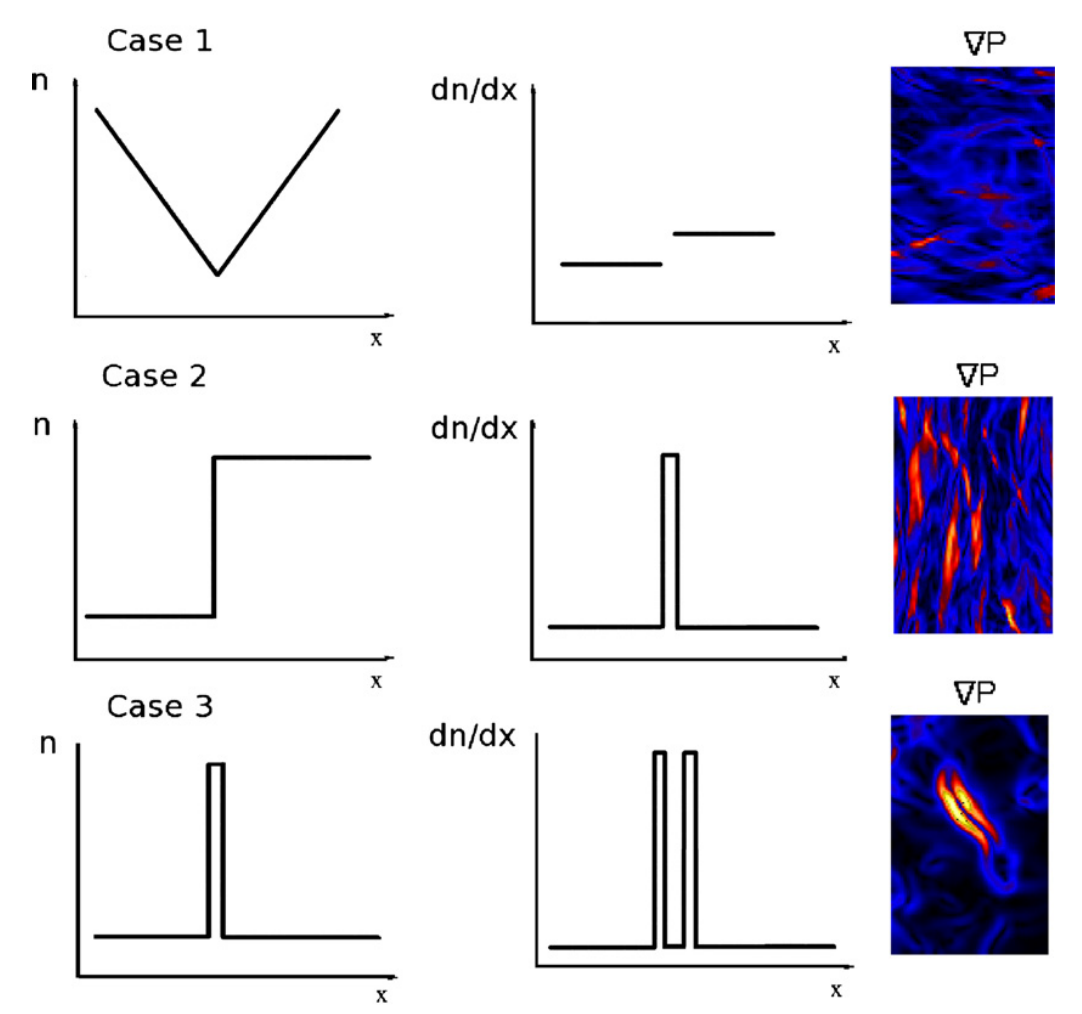
\includegraphics[width=10cm]{figures/PolGradProfiles.png}
\caption{\footnotesize{Schematic example of three possible scenarios for enhancements in a generic image ``n,'' where ``n'' could be $|\vec{P}|$, $\rm RM$, or $\rho/N/{\rm EM}$ (density, column density, emission measure). Case one (top row) shows an example of a H\"older continuous function that is not differentiable at the origin (applicable to all turbulent fields). Case two (middle row) shows an example of a jump resulting from strong turbulent fluctuations along the LOS or weak shocks. Case three (bottom row) shows a delta function profile resulting from interactions of strong shocks. In this case, the derivative gives a double jump profile which produces morphology that is distinctly different from the previous cases. In all cases we show examples from $|\vec{P}|$ simulations. Figure taken from Burkhart (2012).}}
\label{fig:polgradprofiles}
\end{center}
\end{figure}

{\noindent}Of great interest is the question of which quantity is providing the dominant contribution to the structures in $\lvert\nabla\vec{P}\rvert$: $\lvert\nabla n_{e,{\rm LOS}} \rvert$, $\lvert\nabla\vec{B}_{\rm LOS}\rvert$, or both equally? Especially in the case of compressible turbulence, the magnetic energy is correlated with density: denser regions contain stronger magnetic fields due to the compressibility of the gas and the potential dynamo amplification of the magnetic field in dense gas. This causes the magnetic field to follow the flow of plasma if the magnetic tension is negligible. The compressed regions are dense enough to distort the magnetic field lines, enhance the magnetic field intensity, and effectively trap the magnetic energy due to the frozen-in condition. Thus, for the supersonic cases, the intensity of the structures seen in $\lvert\nabla\vec{P}\rvert$ is more pronounced than in the subsonic case. However, in the case of subsonic turbulence, there are no compressive motions. In this case, random fluctuations in density and magnetic field will create structures in $\lvert\nabla\vec{P}\rvert$. It's been shown using MHD simulations that in the case of subsonic turbulence, $\lvert\nabla\vec{P}\rvert$ correlates with $\lvert\nabla\vec{B}\rvert$ while in the supersonic case $\lvert\nabla\vec{P}\rvert$ correlates with density fluctuations. This is because density enhancements are dominant due to shock fronts in the case of supersonic turbulence, while in subsonic turbulence density is marginally incompressible.

{\noindent}\textbf{Polarization gradient (radial component):} The radial component quantifies how changes in polarization intensity contribute to the directional derivative $|\partial\vec{P}/\partial s|$:

\begin{align*}
    \left\lvert\frac{\partial\vec{P}}{\partial s}\right\rvert_\mathrm{rad} = \sqrt{\frac{(Q\frac{\partial Q}{\partial x} + U\frac{\partial U}{\partial x})^2 + (Q\frac{\partial Q}{\partial y} + U\frac{\partial U}{\partial y})^2}{Q^2+U^2}} ~ [{\rm Jy\,pc^{-1}}]
\end{align*}

{\noindent}If changes in polarization intensity are dominant for a feature, then this could imply that the amount of depolarization due to the addition of polarization vectors along the line of sight varies significantly between different positions, and it follows that the medium producing the polarized emission may be very turbulent. This is true for both thermal dust emission and for synchrotron emission.

{\noindent}\textbf{Polarization gradient (tangential component):} The tangential component quantifies how changes in polarization angle, weighted by polarization intensity, contribute to the directional derivative $|\partial\vec{P}/\partial s|$:

\begin{align*}
    \left\lvert\frac{\partial\vec{P}}{\partial s}\right\rvert_\mathrm{tan} = \sqrt{\frac{(Q\frac{\partial U}{\partial x} - U\frac{\partial Q}{\partial x})^2 + (Q\frac{\partial U}{\partial y} - U\frac{\partial Q}{\partial y})^2}{Q^2+U^2}} ~ [{\rm Jy\,pc^{-1}}]
\end{align*}

{\noindent}If changes in polarization angle are dominant, then this could indicate changes in the regular magnetic field threading the observed region, as this would produce significant changes in the emitted polarization angle in the case of thermal dust emission or synchrotron emission. Additionally, changes in the regular magnetic field may also cause the amount of Faraday rotation along different lines of sight to vary significantly, in the case of synchrotron emission.

{\noindent}\textbf{Polarization gradient direction $(\mathrm{arg}\vec\nabla\vec{P})$:} The direction of the \textit{polarization gradient} at a given spatial position defined as

\begin{align*}
    \mathrm{arg}(\vec\nabla\vec{P}) \equiv \arctan \left[ \mathrm{sign} \left(\dfrac{\partial Q}{\partial x}\dfrac{\partial Q}{\partial y} + \dfrac{\partial U}{\partial x}\dfrac{\partial U}{\partial y}\right) \dfrac{\sqrt{\left(\dfrac{\partial Q}{\partial y}\right)^2 + \left(\dfrac{\partial U}{\partial y}\right)^2}}{\sqrt{\left(\dfrac{\partial Q}{\partial x}\right)^2 + \left(\dfrac{\partial U}{\partial x}\right)^2}} \right] ~ [{\rm rad}],
\end{align*}

{\noindent}where $Q$ and $U$ are the complex \textit{Stokes vectors}.

{\noindent}\textbf{Polarization horizon:} The furthest distance we can see diffuse polarized emission. This quantity is a function of the instrumental features (i.e., beam size, observing frequency), as well as of the physical conditions of the probed medium (causing an intrinsic degree of depolarization), and depends on the viewing direction in the Milky Way. The smaller the beam and/or the higher the observing frequency, the farther the polarization horizon; the brighter and/or more coherent the synchrotron emission, the farther the corresponding polarization horizon.

{\noindent}\textbf{Polarized surface brightness ($P(\lambda^2)$):} 

\begin{align*}
    P(\lambda^2) = p(\lambda^2)I(\lambda^2) = Q + iU ~ [{\rm Jy}],
\end{align*}

{\noindent}where $p(\lambda^2)$ is the polarization fraction, $I(\lambda)$ is the total surface brightness, and $Q$ and $U$ are the complex Stokes vectors. The absolute value of this complex vector is given by

\begin{align*}
    \lvert\lvert P(\lambda^2) \rvert\rvert = \sqrt{Q^2 + U^2} ~ [{\rm Jy}],
\end{align*}

{\noindent}where $Q$ and $U$ are the complex Stokes vectors.

{\noindent}\textbf{Poloidal magnetic field:} Often the GMF is expressed in cylindrical coordinates ($\theta, r, z$). The \textit{poloidal magnetic field} refers to the axisymmetrical field structure around $z$ (without $\vec{B}_\theta$ components) such as dipole fields.

{\noindent}\textbf{Power spectrum ($P(k)$):} Describes the distribution of power into frequency components composing that signal defined as

\begin{align*}
    P(k) = \hat{f}(k){\hat{f}(k)}^*,
\end{align*}

{\noindent}for wavenumber $k$ where $\hat{f}(k)$ denotes the \textit{Fourier transform} (FT) and ${\hat{f}(k)}$ its \textit{complex conjugate}. The power spectrum is the \textit{Fourier transform} (FT) of the \textit{autocorrelation function}.

{\noindent}\textbf{Prandtl number:} The ratio of momentum diffusivity (kinematic viscosity) to thermal diffusivity:

\begin{align*}
    {\rm Pr} = \frac{\nu}{\alpha} = \frac{\mu c_p}{k} ~ [{\rm dimensionless}],
\end{align*}

{\noindent}where $\nu=\mu/\rho$ is the momentum diffusivity (kinematic viscosity) in ${\rm m^2\,s^{-1}}$, $\alpha=k/(c_p\rho)$ is the thermal diffusivity in ${\rm m^2\,s^{-1}}$, $\mu$ is the dynamic viscosity in ${\rm Ps\,s}$, $k$ is the thermal conductivity in ${\rm W\,m^{-1}\,K}$, $c_p$ is the specific heat in ${\rm J\,kg^{-1}\,K}$, and $\rho$ is the density in ${\rm kg\,m^{-3}}$.

{\noindent}\textbf{Power spectrum:} The power spectrum is defined as:

\begin{align*}
    P(k) = \sum_k \tilde{F}(k)\cdot\tilde{F}^*(k),
\end{align*}

{\noindent}where $k$ is the wavenumber and $\tilde{F}(k)$ is the Fourier transform of the field under study (e.g., density, kinetic energy, magnetic energy etc.). This equation demonstrates a critical limitation of the Fourier power spectrum: it contains only the Fourier amplitudes and neglects the Fourier phases. This is problematic for studies ofMHD turbulence because interactions among MHD waves can produce correlations in Fourier phases which are completely missed by the power spectrum. Furthermore, the degree of phase coherence or randomness in MHD turbulence is important for MHD wave-wave interactions and particle transport.

{\noindent}\textbf{$Q-U$ plane:} Translations and rotations within the $Q-U$ plane can result from one or more of a smooth distribution of intervening polarized emission, a uniform screen of foreground \textit{Faraday rotation}, and the effects of missing large-scale structure in an interferometric data set.

{\noindent}\textbf{Random magnetic field:} See \textit{turbulent magnetic field}. 

{\noindent}\textbf{Rayleigh-Taylor instability:} Also known as magnetic buoyancy.

{\noindent}\textbf{Reynolds number ($R_e$):}  The Reynolds number is the ratio of an eddy turnover rate and the viscous dissipation rate. Therefore large $R_e$ correspond to negligible viscous dissipation of large eddies over the eddy turn over time. It is an important dimensionless quantity in fluid mechanics used to help predict flow patterns in different fluid flow situations which characterizes the relative importance of inertial (resistant to change or motion) and viscous (heavy and gluey) forces:

\begin{align*}
    {\rm Re} = \frac{\rho vL}{\mu} ~ [{\rm dimensionless}],
\end{align*}

{\noindent}where $\rho$ is the density in ${\rm kg\,m^{-3}}$, $v$ is the velocity in ${\rm m\,s^{-1}}$, $L$ is the characteristic length in ${\rm m}$, and $\mu$ is the dynamic viscosity coefficient in ${\rm Ps\,s}$. At low Reynolds numbers, flows tend to be dominated by laminar (sheet-like) flow, while at high Reynolds numbers, turbulence results from differences in the fluid's speed and direction, which may sometimes intersect or even move counter to the overall direction of the flow (eddy currents).

\begin{figure}[h]
    \floatbox[{\capbeside\thisfloatsetup{capbesideposition={right,top},capbesidewidth=4cm}}]{figure}[\FBwidth]
    {\caption{\footnotesize{Flows at varying Reynolds number Re. In each panel, a fluid that has been dyed red is injected from the top into the clear fluid on the bottom. The fluids are glycerin-water mixture, for which the viscosity can be changed by altering the glycerin to water ratio. By changing the viscosity and the injection speed, it is possible to alter the Reynolds number of the injected flow. The frames show how the flow develops as the Reynolds number is varied. This image is a still from the National Committee for Fluid Mechanics Film series (Taylor, 1964), which, once you get past the distinctly 1960s production values, are a wonderful resource for everything related to fluids.}}
    \label{fig:variablezones}}
    {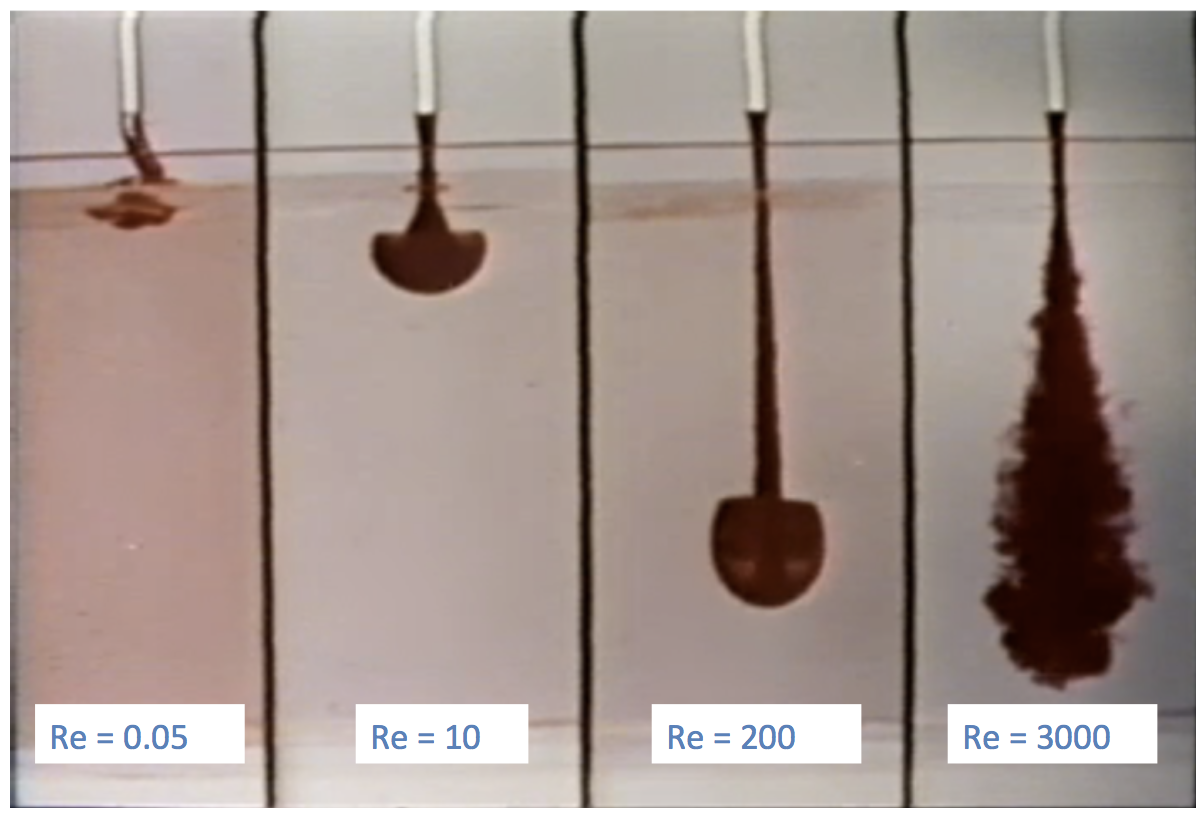
\includegraphics[width=10cm]{figures/ReynoldsNumber.png}}
\end{figure}

{\noindent}\textbf{Rolling Hough Transform (RHT):} A machine vision algorithm designed for detecting and parameterizing linear structure in astronomical data, originally applied to HI images. The detection of astronomical linear structure is approached in various ways depending on the context. Because HI structures are not objects with distinct boundaries, the problem is fundamentally different from many others. As these diffuse HI fibers were not formed by gravitational forces, there is no reason to require that they must be, or bridge, local overdensities. Indeed, these fibers are found often to be in groups of parallel structures, very unlike the cosmic web. Thus, methods developed for gravitationally dominated systems are not optimal for these purposes. The RHT is, as its name suggests, a modification of the Hough transform. The Hough transform was first introduced in in a patent for the detection of complex patterns in bubble chamber photographs. It was soon recognized as a powerful line detection technique, and has found wide applications in image processing and machine vision. The adaption of the Hough transform with the RHT is a rolling version that is particularly well suited to the detection and quantization of specific linear features in astronomical data. The RHT does not merely identify fibers; it encodes the probability that any given image pixel is part of a coherent linear structure. This allows the user to quantify the linearity of regions of sky without specifying fibers as discrete entities. The RHT operates on two-dimensional data and is designed to be sensitive to linear structure irrespective of the overall brightness of the region. The first step is to unsharp mask the image. The image is convolved with a two-dimensional top-hat smoothing kernel of a user-defined diameter, $D_K$. The smoothed data is then subtracted from the original data  and the resulting map is thresholded at 0 to obtain a bitmask. The subtraction of the smoothed component can be considered a suppression of large-scale structure, or a high-pass Fourier filter. Each straight line is parameterized in terms of the angle $\theta$ of its normal, and its minimum Euclidean distance from the origin $\rho$,

\begin{align*}
    \rho = x\cos\theta+y\sin\theta ~ [{\rm pixels}].
\end{align*}

{\noindent}Every possible line in the image space is uniquely specified by a point in the $\rho-\theta$ space. The RHT mapping is performed on a circular domain, diameter $D_W$, centered on each image-space pixel $(x_0,y_0)$ in turn. Then a Hough transform is performed on this area, limited to $\rho=0$. Thus the $\rho-\theta$ space is reduced to a one-dimensional space on $\theta$ for each pixel. All intensity over a set intensity threshold $Z$ is stored as $R(\theta,x_0,y_0)$: RHT intensity as a function of $\theta$ for that pixel. $Z$ is a percentage. In every direction $\theta$, $Z\times D_W$ pixels must contain signal in order for the transform to record the data in that direction. We use the canonical binning for the number of theta bins:

\begin{align*}
    n_\theta = \left[\pi\frac{\sqrt{2}}{2}(D_W-1)\right] ~ [{\rm dimensionless}].
\end{align*}

{\noindent}By iterating (``rolling'') over the entire image space we produce the RHT output, $R(\theta,x,y)$. A visualization of the linear structures identified by the RHT, the \textbf{backprojection $R(x,y)$}, is obtained by integrating $R(\theta,x,y)$ over $\theta$:

\begin{align*}
    R(x,y) = \int R(\theta,x,y)\mathrm{d}\theta ~ [{\rm dimensionless}].
\end{align*}

{\noindent}One advantage of the RHT is that the input parameters of the transform can be chosen to highlight specific linear features of interest. One defines, for a given run of the RHT, a smoothing kernel diameter ($D_K$), a window diameter ($D_W$), and an intensity threshold ($Z$). The rolling nature of the RHT ensures that linear structure at least as long as $D_W$ will be identified. Thus $D_W$, along with the $Z$, sets a lower limit for the spatial length of the linear features. Thresholding below 100\% ($Z<1$) reflects the fact that structures can be physically coherent even if they are not visibly connected. $R(\theta,x,y)$ is intensity as a function of angle on a domain $\theta\in[0,\pi)$, as a $0^\circ$ orientation is equivalent to a $180^\circ$ orientation. $R(\theta,x,y)$ can be sampled in a circular region around each star in the field as

\begin{align*}
    R_*(x,y) = \int\int_\mathrm{disk} R(\theta,x,y)\mathrm{d}x\mathrm{d}y ~ [{\rm dimensionless}].
\end{align*}

{\noindent}To estimate the direction of a given region of the backprojection $R_*(\theta,x,y)$, the expectation value is given by

\begin{align*}
    \langle\theta\rangle' = \frac{1}{2}\arctan \left[\frac{\int\sin(2\theta)R_*(\theta)\mathrm{d}\theta}{\int\cos(2\theta)R_*(\theta)\mathrm{d}\theta}\right] ~ [{\rm rad}]
\end{align*}

{\noindent}where the equivalent value is found on the interval $\theta\in[0,\pi)$ via

\begin{align*}
    \langle\theta\rangle = \pi - {\rm mod}(\langle\theta\rangle'+\pi,\pi) ~ [{\rm rad}].
\end{align*}

{\noindent}Linear polarization data can be fully described by either
a polarization angle $\chi$ and polarized intensity $P$ or by the Stokes parameters $Q$ and $U$, where $\chi=(1/2)\arctan(U/Q)$ and $P=\sqrt{Q^2+U^2}$. From the RHT output, similar `Stokes vectors' can be defined via

\begin{align*}
    Q_\mathrm{RHT} = \int\cos(2\theta)R(\theta)\mathrm{d}\theta ~ [{\rm Jy}] \\
    U_\mathrm{RHT} = \int\sin(2\theta)R(\theta)\mathrm{d}\theta ~ [{\rm Jy}].
\end{align*}

{\noindent}This allows for an estimate of the orientation of the magnetic field to be derived solely from HI data via

\begin{align*}
    \theta_\mathrm{RHT} = \frac{1}{2}\arctan\left(\frac{U_\mathrm{RHT}}{Q_\mathrm{RHT}}\right) ~ [{\rm rad}].
\end{align*}

{\noindent}\textbf{Rotation measure (RM):} Characterizes the amount of \textit{Faraday rotation} that polarized light experiences while passing through thermal electrons. Most compact polarized sources like pulsars and extremely compact extragalactic sources show a single value of Faraday rotation which is the RM. This is commonly defined as the slope of the polarization angle $\chi$ versus $\lambda^2$ plot:

\begin{align*}
    {\rm RM} = \frac{\mathrm{d}\chi(\lambda^2)}{\mathrm{d}\lambda^2} ~ [{\rm rad\,m^{-2}}],
\end{align*}

{\noindent}where

\begin{align*}
    \chi = \frac{1}{2}\arctan\left(\frac{U}{Q}\right) ~ [{\rm rad}].
\end{align*}

{\noindent}The RM, then, modifies the polarization angle $\chi$ from it's initial value $\chi_0$ as 

\begin{align*}
    \chi = \chi_0 + \mathrm{RM}\lambda^2 ~ [{\rm rad}].
\end{align*}

{\noindent}The value of $\mathrm{RM}$ is the integral of the line-of-sight component of the magnetic field weighted by the line-of-sight distribution of electron density, given by

\begin{align*}
	\mathrm{RM} = -0.81 \int\limits_\mathrm{source}^\mathrm{observer} n_e \vec{B}\cdot\vec{{\rm d}l} ~ [{\rm rad\,m^{-2}}],
\end{align*}

{\noindent}where $\vec{B}$ has units of $\mu{\rm G}$, $n_e$ has ${\rm cm^{-3}}$, and $\vec{{\rm d}l}$ has ${\rm pc}$. This can also be applied to cosmological scales via

\begin{align*}
	\mathrm{RM} = -0.81 \int\limits_{z_\mathrm{source}}^\mathrm{observer} \frac{n_e(z) \vec{B(z)}}{(1+z)^2} \cdot \frac{\vec{{\rm d}l}}{{\rm d}z} {\rm d}z ~ [{\rm rad\,m^{-2}}],
\end{align*}

{\noindent}where $z_\mathrm{source}$ is the redshift of the source. When observing a distant polarized source, the rotation of its linear polarization angle is due to the contribution of different magneto-ionic regions along the line of sight. The measured RM is a sum of contributions from multiple sources, or regions, such that

\begin{align*}
    {\rm RM} = {\rm RM}_{\rm source} + {\rm RM}_{\rm IGM} + {\rm RM}_{\rm Gal} + {\rm RM}_{\rm noise} ~ [{\rm dimensionless}],
\end{align*}

{\noindent}where ${\rm RM}_{\rm source}$ is the source contribution, ${\rm RM}_{\rm IGM}$ is the contribution from the \textit{intergalactic medium} (IGM), ${\rm RM}_{\rm Gal}$ is the contribution from our Galaxy, and ${\rm RM}_{\rm noise}$ is the measurement uncertainty.

{\noindent}The RM can be measured towards distant extragalactic radio sources and pulsars. The RM of an extragalactic radio source consists of an RM contribution intrinsic to the source, the RM from the intergalactic space from the source to the Galaxy, and the RM within the Galaxy. The first term (i.e., the extragalactic radio source) should be random and hence reasonably small on average, because a source can be randomly oriented in space with any possible field configuration; thus we observe a random quantity. The second term (i.e., the intergalactic source) is negligible on average. Intergalactic magnetic fields are too weak to be detected with current technology. Even if there is a weak field in intergalactic space, an integration over the path-length of the intergalactic magnetic field with random directions with extremely thin gas should give quite a small contribution. Therefore, the common contribution of RMs of extragalactic radio sources is from our own Galaxy. 

{\noindent}The RM does not increase monotonically with distance along the line of sight. Traditionally, the RM is obtained by performing a least-squares fit to the data to determine the slope. There are however three potential problems to this method: (1) the observed polarization angle is only known modulo $\pi$ radians; thus with measurements in only a few wavelength bands, the RM is often ambiguous (known as the \textit{$n\pi$ ambiguity}), (2) polarized emission with different RM values can be present along a single line of sight; the signal from these regions mix, making a single linear fit inappropriate, and (3) faint sources with high RM will be undetectable in individual channels due to low signal to noise and will remain undetectable even after integrating all channels due to \textit{bandwidth depolarization}; thus, no $\chi(\lambda^2)$ data will be available for the traditional linear fit.

{\noindent}\textbf{Rotation measure (RM) synthesis:} A robust method for determining the \textit{Faraday dispersion function} as proposed by Burn (1966). It was seldom used until Brentjens and de Bruyn (2005) who coined the term \textit{RM Synthesis}. This technique involves Fourier transforming the observed \textit{polarized surface brightness} $P(\lambda^2)$ into the \textit{Faraday dispersion function} $F(\phi)$ (also referred to as the \textit{Faraday spectrum}) which is the complex polarized surface brightness as a function of \textit{Faraday depth}. As shown by Burn (1966), the the observed complex polarization vector can be written as $P(\lambda^2)=pI\mathrm{e}^{2i\chi}$, where $p$ is the \textit{polarization fraction} and $I$ is the \textit{Stokes I} vector. Substituting the expression $\chi(\lambda^2)=\chi_0+\phi\lambda^2$ for the polarization angle $\chi$ as a function of Faraday depth $\phi$, we obtain

\begin{align*}
    P(\lambda^2) &= pI\mathrm{e}^{2i(\chi_0+\phi\lambda^2)}\\
    &= pI\mathrm{e}^{2i\chi_0}\mathrm{e}^{2i\phi\lambda^2}\\
    &= \left(pI\mathrm{e}^{2i\chi_0}\right)\mathrm{e}^{2i\phi\lambda^2}\\
    &= F(\phi)\mathrm{e}^{2i\phi\lambda^2} ~ [{\rm Jy}],
\end{align*}

{\noindent}where $F(\phi)$ is the \textit{Faraday dispersion function} which describes the intrinsic polarized flux as a function of Faraday depth. Since the observed polarization originates from emission along all Faraday depths, integrating this over $\phi$ gives the final form

\begin{align*}
    P(\lambda^2) = \int\limits_{-\infty}^\infty F(\phi)\mathrm{e}^{2i\phi\lambda^2}\mathrm{d}\phi ~ [{\rm Jy}].
\end{align*}

{\noindent}Thus there is a simple expression that relates the intrinsic quantity $F(\phi)$ to the observable $P(\lambda^2)$ which takes the form of a Fourier transform. This can now be inverted to obtain the Faraday dispersion function

\begin{align*}
    F(\phi) = \int\limits_{-\infty}^\infty P(\lambda^2)\mathrm{e}^{-2i\phi\lambda^2}\mathrm{d}\lambda^2 ~ [{\rm rad\,m^{-2}}].
\end{align*}

{\noindent}However, one is confronted with a problem: namely, that we cannot observe at wavelengths $\lambda<0$, nor do we observe for all wavelengths $\lambda>0$. To resolve this issue, Brentjens \& de Bruyn (2005) introduce a window function $W(\lambda^2)$ which is non-zero only at wavelengths sampled by the telescope. They show that the observed polarized surface brightness can be rewritten as 

\begin{align*}
    \tilde{P}(\lambda^2) \equiv W(\lambda^2)P(\lambda^2) = W(\lambda^2) \int\limits_{-\infty}^\infty F(\phi)\mathrm{e}^{2i\phi(\lambda^2-\lambda_0^2)}\mathrm{d}\phi ~ [{\rm Jy}],
\end{align*}

{\noindent}and the reconstructed Faraday dispersion function as

\begin{align*}
    \tilde{F}(\phi) \equiv \dfrac{\int\limits_{-\infty}^\infty \tilde{P}(\lambda^2)\mathrm{e}^{-2i\phi(\lambda^2-\lambda_0^2)}\mathrm{d}\lambda^2}{\int\limits_{-\infty}^\infty W(\lambda^2)\mathrm{d}\lambda^2} = F(\phi) * R(\phi) ~ [{\rm rad\,m^{-2}}],
\end{align*}

{\noindent}where $*$ denotes convolution. $\tilde{F}(\phi)$ is an approximate reconstruction of $F(\phi)$. More precisely, it is $F(\phi)$ convolved with $R(\phi)$ after Fourier filtering by the weight function $W(\
lambda^2)$. $R(\phi)$ is the \textit{rotation measure transfer function} (RMTF) which is a crucially important quantity defined by

\begin{align*}
    R(\phi) \equiv \dfrac{\int\limits_{-\infty}^\infty W(\lambda^2)\mathrm{e}^{-2i\phi(\lambda^2-\lambda_0^2)}\mathrm{d}\lambda^2}{\int\limits_{-\infty}^\infty W(\lambda^2)\mathrm{d}\lambda^2} ~ [{\rm rad\,m^{-2}}],
\end{align*}

{\noindent}which is normalized to unity at $\phi=0$. It is a complex valued function. The real part corresponds to the response of the transform parallel to the ($Q,U$) vector at $\lambda_0=\lambda$ while the imaginary part corresponds to the response orthogonal to it. Taking a look at the equations above for $\tilde{F}(\phi)$ and $R(\phi)$, these can be seen as applications of the Fourier shift theorem -- since the shift theorem only affects the argument and not the absolute value of the resulting complex vector function, de-rotating these equations to $\lambda_0\neq0$ does not change their amplitude. The Faraday spectrum is not straightforward to interpret; in particular, there is no direct relationship between Faraday depth and physical depth. Further, the Faraday dispersion function suffers from sidelobes of the main components caused by limited coverage of the observed wavelength space. RM Synthesis is required when multiple emitting and rotating regions are located along the line of sight, as opposed to a single emitting region (i.e., Faraday screen) behind a single rotating region. RM synthesis was applied to an entire field of view for the first time by de Bruyn (1966) using pulsar observations. When applied to a complete field of view instead of just a single line of sight, the output of RM synthesis is referred to as an ``RM cube''. RM synthesis is characterized by four parameters: (1) the resolution in Faraday space, which is inversely proportional to the coverage in wavelength space, (2) the maximum observable of a point-like source in Faraday space, which is inversely proportional to the width of a single frequency channel, (3) the maximum width of extended structures in Faraday space (Faraday rotating and synchrotron emitting sources), which is inversely proportional to the square of the minimum observable wavelength; wide-band observations at long wavelengths yield high resolution in Faraday space but cannot detect extended structures, and (4) the ratio of maximum to minimum wavelengths which is crucial to recognize a range of different scales in Faraday space. Table \ref{table:rmsynthesis} these parameters for a variety of radio telescopes. The highest resolution in Faraday space are for those with the largest wavelength coverage (LOFAR and SKA) while the largest range of scales in Faraday space are for those with the greatest ratio of maximum to minimum wavelengths (ATCA, JVLA, SKA).

\begin{table}[h]
\begin{center}
\captionof{table}{\footnotesize{Spectral ranges of various radio telescopes and parameters crucial for RM synthesis. Table from Beck et al. (2012).}} \label{table:rmsynthesis}
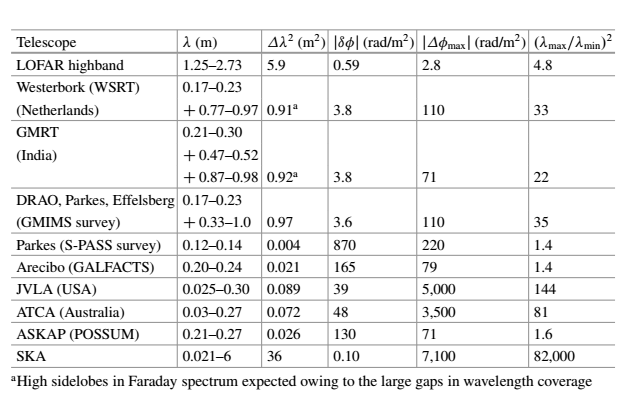
\includegraphics[width=12cm]{figures/RMsynthesis.png}
\end{center}
\end{table}

{\noindent}\textbf{Rotation measure transfer function (RMTF):} A crucially important quantity introduced by de Bruyn (1966) and defined by

\begin{align*}
    R(\phi) \equiv \dfrac{\int\limits_{-\infty}^\infty W(\lambda^2)\mathrm{e}^{-2i\phi(\lambda^2-\lambda_0^2)}\mathrm{d}\lambda^2}{\int\limits_{-\infty}^\infty W(\lambda^2)\mathrm{d}\lambda^2} ~ [{\rm rad\,m^{-2}}],
\end{align*}

{\noindent}which is normalized to unity at $\phi=0$. For a simple weight function $W(\lambda^2)$ that is a top-hat (boxcar) fuction centered on $\lambda_c^2$ with width $\Delta\lambda^2 = \lambda_2^2-\lambda_1^2$, the corresponding RMTF is a sinc function with a phase wind:

\begin{align*}
    R(\phi) = e^{i\phi\lambda_c^2}\left(\dfrac{\sin(\phi\Delta\lambda^2)}{\phi\Delta\lambda^2}\right) ~ [{\rm rad\,m^{-2}}]
\end{align*}

{\noindent}It is a complex valued function; the real part corresponds to the response of the transform parallel to the ($Q,U$) vector at $\lambda_0=\lambda$ while the imaginary part corresponds to the response orthogonal to it. Ideally, the response in the entire main peak of the RMTF should be parallel to the actual polarization vector at $\lambda_0$. Brentjens \& de Bruyn (2005) show that this optimal choice of $\lambda_0^2$ is the mean of the sampled $\lambda^2$ values weighted by $W(\lambda^2)$. However, since the shift theorem of Fourier theory only applies to the argument, changing the value of $\lambda_0$ will not change the absolute value of the RMTF. A drawback of having $\lambda_0\neq0$ is that the polarization angle that one derives still needs to be transformed to a polarization angle at $\lambda=0$ if one wants information on the electric or magnetic field direction of the source. In the case of a high $S/N$, this is easy:

\begin{align*}
    \chi_0 = \chi(\lambda_0^2) - \phi\lambda_0^2 ~ [{\rm rad}].
\end{align*}

{\noindent}However, if the $S/N$ is low, the uncertainty in $\phi$ usually prevents accurate de-rotation to $\lambda=0$. 

{\noindent}\textbf{Saliency map:} In computer vision, a saliency map is an image that shows each pixel's unique quality. The goal of a saliency map is to simplify and/or change the representation of an image into something that is more meaningful and easier to analyze. For example, if a pixel has a high grey level or other unique colour quality in a colour image, that pixel's quality will show in the saliency map and in an obvious way..

{\noindent}\textbf{Scintillation:}

{\noindent}\textbf{Second moment:} See \textit{variance}.

{\noindent}\textbf{Skewness ($\gamma_x$):} The degree of asymmetry of a distribution, and can be quantified to define the extent to which a distribution differs from a normal distribution. Skewness is defined as

\begin{align*}
    \gamma_x = \frac{1}{N} \sum_{i=1}^N \left(\frac{x_i-\mu_x}{\sigma}\right)^4 -3 ~ [{\rm dimensionless}],
\end{align*}

{\noindent}where $\mu_x$ is the statistical mean and $\sigma$ is the standard deviation. It can be negative, positive, zero or undefined, and like the \textit{kurtosis}, is a dimensionless quantity.

{\noindent}\textbf{Sonic Mach number ($\mathcal{M}_s$):} The ratio of the flow speed to that of the sound speed of the \textit{interstellar medium} given by

\begin{align*}
    \mathcal{M}_s = \left\langle\frac{\lvert\vec{v}\rvert}{c_s}\right\rangle ~ [{\rm dimensionless}],
\end{align*}

{\noindent}where $|\vec{v}|$ is the local velocity and $c_s$ is the sound speed. This number is a commonly used parameter of turbulence used to obtain information on gas compressibility and magnetization. The statistical determination of the sonic Mach number is possible because of the relationship between turbulence regimes and the probability distribution functions (PDFs) of the image intensity distribution. The probability distribution function of an image distribution gives the frequency of occurrence of intensities values and can be described by the main statistical moments: mean, variance, skewness, and kurtosis. The higher order moments (skewness and kurtosis) measure the degree of deviation of the PDF from a Gaussian, and are sensitive to the imprints of turbulence encoded in the image intensity distribution. For this reason, their use constitutes a common diagnostic for astrophysical turbulence. Using polarization gradients of \textit{synchrotron radiation}, it was shown by Gaensler (2011) that the turbulence of the WIM has a relatively low \textit{sonic Mach number}, $\mathcal{M}_s\lesssim2$.

{\noindent}\textbf{Spectral index ($\alpha$):} A measure of the dependence of radiative flux density on frequency. Between any two frequencies ($\nu$) with total intensity ($I$), the spectral index is given by:

\begin{align*}
    \alpha \equiv \frac{\log(I_1/I_2)}{\log(\nu_1/\nu_2)} ~ [{\rm dimensionless}].
\end{align*}

{\noindent}If flux does not follow a power-law distribution, the spectral index itself is a function of frequency. In the radio regime, a spectral index of $\alpha=0-2$ indicates thermal emission while a steep negative spectrum indicates synchrotron radiation.

{\noindent}\textbf{Spectral correlation function ($S_{x,y}$):} The average over all neighboring spectra of the normalized rms difference between \textit{brightness temperatures} $T_b$ for pairs of velocity channels $(v_i,v_j)$ defined as

\begin{align*}
    S_{x,y} \equiv S_{v_i,v_j} = \frac{1}{n}\sum_{a=1}^n T_b([x,y]_a,v_i)T_b([x,y]_a,v_j),
\end{align*}

{\noindent}where $n$ is the number of positions in the map. A histogram of $S_{x,y}$ reveals the autocorrelation properties: if $S_{x,y}$ is close to unity, the spectra do not vary much.

{\noindent}\textbf{Spectral irradiance ($E_\nu(T)~{\rm or}~E_\lambda(T)$):} The \textit{Planck function} multiplied by the total solid angle of a sphere ($4\pi\,{\rm sr}$) which describes the power per area per frequency or the power per area per wavelength:

\begin{align*}
    E_\nu(T) = \left(\frac{8\pi h\nu^3}{c^2}\right) \frac{1}{e^{h\nu/k_BT}-1} ~ [{\rm W\,m^{-2}\,Hz^{-1}}] \\
    E_\lambda(T) = \left(\frac{8\pi hc^2}{\lambda^5}\right) \frac{1}{e^{hc/\lambda k_BT}-1} ~ [{\rm W\,m^{-2}\,m^{-1}}].
\end{align*}

{\noindent}\textbf{Starlight polarization:} The polarization of initially unpolarized starlight which becomes polarized as it passes through dust grains aligned by an external magnetic field. Paramagnetic materials have unpaired electrons which, when in the presence of an external magnetic field such as the interstellar magnetic field, align in the same direction causing grain alignment. In the case of elongated dust grains, if the shortest axis is aligned with the direction of the magnetic field, then the grains will absorb light polarized along the long axis of the grain which is perpendicular to the field. This results in transmitted radiation having a polarization direction parallel to the magnetic field. Optical polarization of starlight was first imaged by Hall \& Mikesell (1949) and Hiltner (1949). They found that polarized light from nearby stars had similar orientation, indicating that the polarizing mechanism was a source other than the individual stars. Shortly thereafter, Davis \& Greenstein (1951) published a theory on the origin of polarized starlight. They proposed that an elongated dust grain spinning about its shortest axis would have a preferred orientation when located in a magnetic field. Starlight polarization is most useful for detecting magnetic fields in the Solar neighbourhood out to about $1-3\,{\rm kpc}$. The same large-scale alignment of spinning, aspherical dust grains that causes starlight polarization also causes \textit{infrared polarization}.

{\noindent}\textbf{Stellar wind bubble (SWB):} A cavity light years across filled with hot gas blown into the interstellar medium by high-velocity (several thousand ${\rm km\,s^{-1}}$) stellar wind from a single massive O or B star. The heliosphere blown by the Solar wind, within which all of the major planets of the Solar System are embedded, is a small example of a stellar wind bubble.

{\noindent}\textbf{Stochastic system:}

{\noindent}\textbf{Stokes parameters:} Polarization is usually observed and characterized in terms of the Stokes parameters: $I, Q, U,$ and $V$. Of primary interest are usually the linear polarization parameters $Q$ and $U$. While Stokes $Q$ and $U$ are observationally convenient, they are coordinate system dependent so they do not couple naturally to the underlying physics. For this, the E-mode and B- mode representation of orthogonal polarization components are sometimes ideal.

{\noindent}\textbf{Stokes I ($I$):} A measure of the total intensity of radio emission.

{\noindent}\textbf{Stokes Q ($Q$):} A measure of the linear polarization of radio emission defined as

\begin{align*}
    Q = P\cos(2\chi) ~ [{\rm Jy}],
\end{align*}

{\noindent}where $P$ is the \textit{polarized intensity} and $\chi$ is the polarization angle. The images of Stokes Q (and \textit{Stokes U}) as well as the \textit{linear polarized intensity} $P\equiv\sqrt{(Q^2+U^2)}$ are often filled with complex structures that bear little resemblance to the \textit{Stokes I} image of total intensity. The intensity variations seen in $Q$ (as well as $U$ and $P$) are the result of small-scale angular structure in the \textit{Faraday rotation} induced by ionized gas, and are thus an indirect representation of turbulent fluctuations in the free-electron density and magnetic field throughout the \textit{interstellar medium}.

{\noindent}\textbf{Stokes U ($U$):} A measure of the linear polarization of radio emission defined as

\begin{align*}
    U = P\sin(2\chi) ~ [{\rm Jy}],
\end{align*}

{\noindent}where $P$ is the \textit{polarized intensity} and $\chi$ is the polarization angle. The images of Stokes U (and \textit{Stokes Q}) as well as the \textit{linear polarized intensity} $P\equiv\sqrt{(Q^2+U^2)}$ are often filled with complex structures that bear little resemblance to the \textit{Stokes I} image of total intensity. The intensity variations seen in $U$ (as well as $Q$ and $P$) are the result of small-scale angular structure in the \textit{Faraday rotation} induced by ionized gas, and are thus an indirect representation of turbulent fluctuations in the free-electron density and magnetic field throughout the \textit{interstellar medium}.

{\noindent}\textbf{Stokes V ($V$):} A measure of circular polarization of radio emission. If $V>0$, then the electromagnetic wave is right-handed circularly polarized (RCP), while if $V<0$, then the electromagnetic wave is left-handed circularly polarized (LCP). Stokes V is related to the line-of-sight magnetic field in the following manner:

\begin{align*}
    V(\nu) \propto B_\parallel \times \frac{\mathrm{d}I}{\mathrm{d}\nu} ~ [{\rm Jy}],
\end{align*}

{\noindent}where $I$ is \textit{Stokes I} and $\nu$ is the observed frequency.

{\noindent}\textbf{Striation:} 

{\noindent}\textbf{Str\"{o}mgren sphere:} A sphere of ionized hydrogen (HII) around young OB stars.

{\noindent}\textbf{Structure function ($S_p(\delta r)$):} The structure function of order $p$ for an observable $A$ is given by

\begin{align*}
    S_p(\delta r) = \langle\lvert A(r)-A(r+\delta r)\rvert^p\rangle,
\end{align*}

{\noindent}for position $r$ and position increment $\delta r$. The power-law fit to this, $S_p(\delta e)\propto\delta r^{\upzeta}_p$, gives the slope $\zeta_p$.

{\noindent}\textbf{Superbubble:} Also known as a \textit{supershell}. Supershells and superbubbles are the largest classification of HI shells, with radii between $10^2$ and $10^3\,{\rm pc}$, blown into the ISM by multiple SNe and stellar winds from clusters and associations of massive O and B stars. Such objects occupy an intermediate size-scale within the ISM; a scale at which the role of magnetic fields in the \textit{magneto-ionic medium} (MIM) is not well understood. Supershells are most commonly found in HI surveys, and appear as cavities in the neutral hydrogen; but they can also have multi-wavelength properties. Supershells can have associated emission in H$\alpha$, soft X-rays, far ultra-violet, polarized radio continuum, and $100\,\mu{\rm m}$. It is thought that once bubbles expand far enough to break out of the gas of the Galactic plane, the shell breaks open into a Galactic chimney, allowing the flow of hot gas into the halo. This transition from bubble to chimney is slowed by the presence of magnetic fields, which tend to confine the expanding shell in the disc.

A superbubble behaves qualitatively like an individual supernova remnant, except that it has a continuous supply of energy. For the first $3\,{\rm Myrs}$ at least, their energy supply is exclusively due to stellar winds, whose cumulative power rises rapidly with time. Supernovae start exploding after $\gtrsim3\,{\rm Myrs}$, and within $\sim2\,{\rm Myrs}$, they overpower the stellar winds. From then on, the successive supernovae explosions continue to inject energy into the superbubble at a slowly decreasing rate, depending on the \textit{initial mass function} (IMF) of the progenitor stars, until $\sim40\,{\rm Myrs}$. Altogether, stellar winds account for a fraction comprising between $\sim12\%$ and $\sim17\%$ of the total energy input. The Solar System lies near the center of an old superbubble known as the \textit{Local Bubble} whose boundary can be traced by a sudden rise in dust extinction.

{\noindent}\textbf{Supernova:} A supernova is a transient astronomical event that occurs during the last stellar evolutionary stages of a star's life, either a massive star or a white dwarf, whose destruction is marked by one final, titanic explosion. Supernovae come in two types. \textit{Type-I} supernovae arise from old, degenerate low-mass stars which supposedly are accreting from a companion and undergoes a thermonuclear instability upon accumulation of a critical mass. \textit{Type-II} supernovae arise from young stars with initial masses $\gtrsim8\,{\rm M}_\odot$ whose core gravitationally collapses once it has exhausted all of its fuel. Like the bright, massive stars, Type-II supernovae are tightly confined to the spiral arms while Type-I supernovae have a more spread-out distribution similar to the general stellar population. Type-I supernovae are less frequent than their Type-II counterparts. All of them are uncorrelated in space and have basically the same repercussions on the ISM as isolated Type-II supernovae. The hot gas created by supernovae explosions (and stellar winds) in the Galactic disk rises into the halo under the influence of its own buoyancy. In the course of its upward motion, it cools down (almost adiabatically at first, then by radiative transport), and eventually condenses into cold neutral clouds. Once formed, these clouds fall ballistically towards the Galactic plane. This convective cycle of interstellar material between the disk and the halo is known as the \textit{Galactic fountain}.

{\noindent}\textbf{Supershell:} See \textit{superbubble}.

{\noindent}\textbf{Synchrotron radiation:} The radio emission produced by relativistic \textit{cosmic rays} when accelerated radially (e.g., by magnetic fields) which is one of the most commonly used tracers of the Galactic magnetic field. Synchrotron radio emission is a tool to measure the total strength of magnetic field on the assumption that the magnetic energy-density (pressure) is in equipartition with the thermal and cosmic ray energy densities. This method requires information about the depth of emitting region in order to calculate the synchrotron emissivity per volume, as the intensity is an integration of the emissivity along the line-of-sight.

{\noindent}Synchrotron emission has a steep spectral index of $\alpha\sim-2.75$, which results in much brighter emission at lower frequencies (this applies to both linear polarization and total intensity). For a single electron, the critical frequency of synchrotron radiation can be expressed as

\begin{align*}
    \nu_c = \dfrac{3}{4\pi}\dfrac{q}{mc}\gamma^2(B\sin\theta)~[{\rm Hz}],
\end{align*}

{\noindent} or

\begin{align*}
\nu_c \sim \gamma^2 \frac{eB}{2\pi m_0} ~ [{\rm Hz}],
\end{align*}

{\noindent}where $\gamma$ is the \textit{Lorentz factor}, $e$ and $m_0$ are the charge and rest mass of the cosmic ray electron, and $B$ is the magnetic field strength. As the cosmic ray gyrates around the local magnetic field, it generates the synchrotron radiation beamed within the shape of a cone at an angle of 

\begin{align*}
    \theta = \pm \frac{m_cc^2}{E} ~ [{\rm rad}].
\end{align*}

{\noindent}On the surface of the cone, the radiation is 100\% linearly polarized with an electric field $E$ that has a direction of $-\mathbf{v\times B}$. Synchrotron radiation from the Galaxy was the first emission detected in radio astronomy by Jansky (1933), however, it was not until the 1950's when detailed radio maps of the Galaxy were produced that the connection was made between radio emission and the synchrotron mechanism. Linear polarization of synchrotron radiation can be used to trace ordered magnetic fields in the plane of the sky ($B_\perp$). Unpolarized synchrotron emission can be indicative of a turbulent magnetic field causing depolarization via Faraday rotation of thermal electrons (synchrotron radiation cannot cause Faraday rotation). The radiated power from an accelerating charge $q$ with mass $m$ by a magnetic field $B$ at an observing frequency $\nu$ is

\begin{align*}
    P = \frac{2}{3}\dfrac{q^4}{m^2c^5}(\gamma\nu)^2(B\sin\theta)^2 ~ [{\rm Jy}].
\end{align*}

{\noindent}Since synchrotron radiation is proportional to the charge-to-mass ratio, electrons dominate synchrotron radiation over protons and ions by several orders of magnitude. Synchrotron radiation peaks at a characteristic frequency of

\begin{align*}
    \nu_c = \dfrac{3}{4\pi}\dfrac{q}{mc}\gamma^2(B\sin\theta)~[{\rm Hz}].
\end{align*}

{\noindent}For radio observations with typical frequencies at or above tens of ${\rm MHz}$ and with typical magnetic field strengths of order $\mu$G, the observed population of synchrotron electrons have $\gamma\gg1$. Synchrotron emission has a steep negative spectral index in the radio regime. Assuming that the electrons are moving isotropically, Le Roux (1961) showed that the maximum intrinsic degree of polarization (i.e., polarization fraction) of synchrotron radiation from plasma in a uniform magnetic field is a function of the electron's spectral index $\gamma$ given by

\begin{align*}
    p = \frac{3\gamma + 3}{3\gamma+7} ~ [{\rm dimensionless}],
\end{align*}

{\noindent}independent of frequency and observing angle. Using observations of the Crab Nebula, Woltjer (1958) and Westfold (1959) showed that $\gamma\approx5/3$ and therefore $p\approx67\%$. Le Roux (1961) gives a full derivation of synchrotron radiation. Figure \ref{figure:408mhz} shows the Galactic synchrotron emission at $408\,{\rm MHz}$.

\begin{figure}[h]
\begin{center}
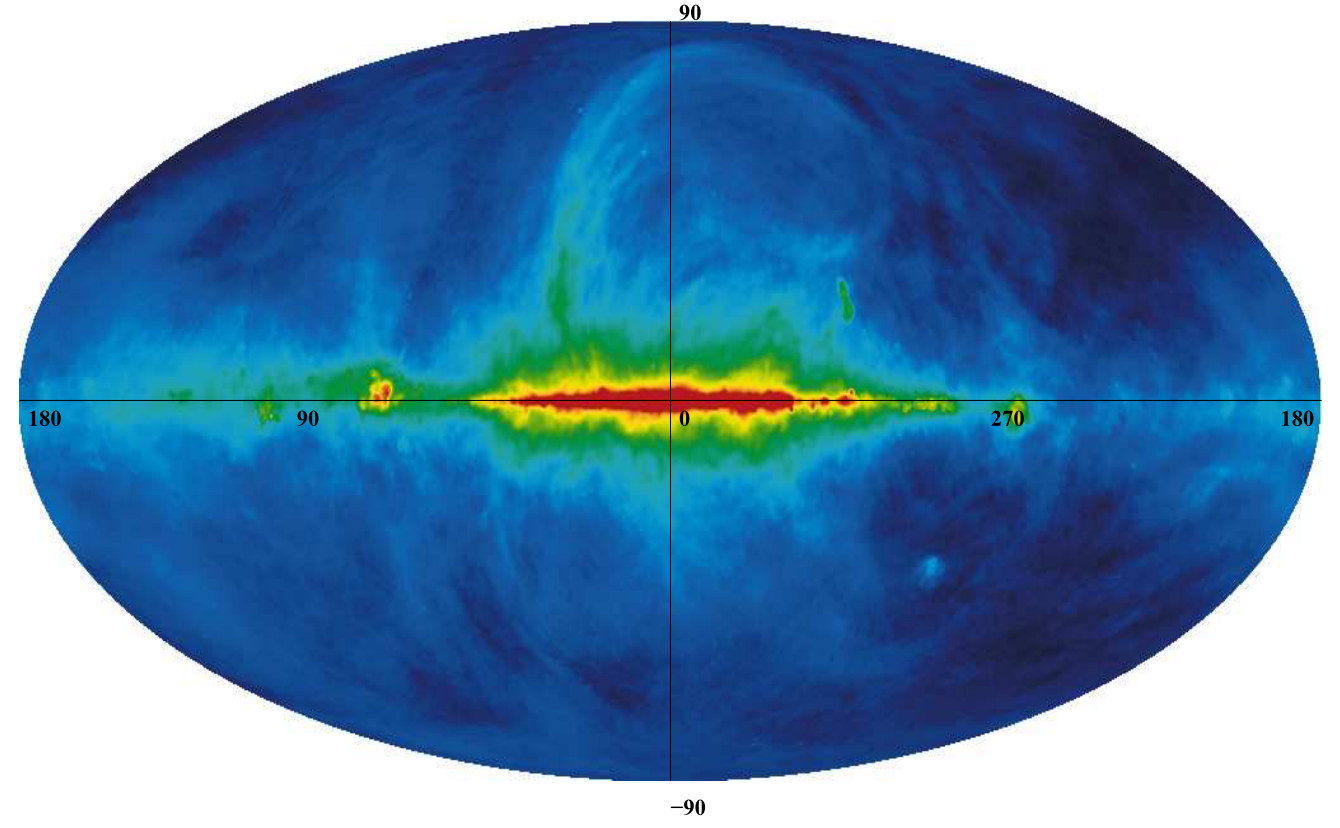
\includegraphics[width=15cm]{figures/408MHz.png}
\caption{\footnotesize{The synchrotron emission at $408\,{\rm MHz}$ across the entire sky in Galactic coordinates. As expected, the emission is concentrated along the Galactic plane. However, the feature known as Loop I, is clearly arching up from $\ell=55^\circ$ towards the North Galactic Pole. This Figure is adapted from Haslam et al. (1981). Figure taken from Newton-McGee (2009).}}
\label{figure:408mhz}
\end{center}
\end{figure}

{\noindent}\textbf{Taylor scale:}

{\noindent}\textbf{Temperature B-mode (TB) correlation:} A positive signal in the Temperature B-mode ($TB$) cross spectrum roughly consistent with a power law as a function of multipole moment $\ell$ for $\ell\lesssim600$. This non-zero $TB$ measurement was originally made using angular power spectra computed from $353\,{\rm GHz}$ intensity and polarization maps of Planck HFI data, where the dominant polarized foreground is that from thermal dust emission (Planck Collaboration XI 2018; Planck Collaboration Int. LIV 2018; Planck Collaboration Int. XXX 2016). Physical arguments predict the $TB$ and $EB$ signals from the CMB to be statistically consistent with zero (e.g., Zaldarriaga \& Seljak 1997). Thus the two most likely sources for the non-zero $TB$ signal are residual systematics in the data, and/or a non-zero $TB$ contribution from Galactic thermal dust emission. An analysis that computed $TB$ and $EB$ power spectra and investigated how dust total intensity, polarization fraction, and polarization angle contribute to the $TB$ signal showed that that polarization angle was the key component in producing the observed Planck $353\,{\rm GHz}$ non-zero $TB$ spectrum (Weiland et al., 2019). This supported the conclusion that the Planck $353\,{\rm GHz}$ non-zero $TB$ spectrum is a physical property of Galactic foreground dust polarization.

{\noindent}\textbf{Third moment:} See \textit{skewness}.

{\noindent}\textbf{Toroidal magnetic field:} Often the GMF is expressed in cylindrical coordinates ($\theta, r, z$). The \textit{toroidal magnetic field} refers to the structures (without $\vec{B}_z$ components) confined to a plane parallel to the Galactic plane. The toroidal fields possibly extend to the inner Galaxy, even towards the central molecular zone (CMZ).

{\noindent}\textbf{Tsallis distribution:} A function that can be fit to incremental probability distribution functions (PDFs) of turbulent density, magnetic field, and velocity. The Tsallis distribution was originally derived by Tsallis (1988) as a means to extend traditional Boltzmann-Gibbs mechanics to fractal and multifractal systems. The complex dynamics of multi-fractal systems apply to many natural environments, such as ISM turbulence. The Tsallis function of an arbitrary incremental PDF $\Delta f$ has the form

\begin{align*}
    R_q = a \left[ 1+(q-1) \dfrac{\Delta f(r)^2}{w^2} \right]^{-1/(q-1)}.
\end{align*}

{\noindent}The fit is described by three dependent variables. The $a$ parameter describes the amplitude while $w$ is related to the width or dispersion of the distribution. Parameter $q$, referred to as the ``non-extensivity parameter'' or ``entropic index'' describes the sharpness and tail size of the distribution. The Tsallis fit parameters are in many ways similar to statistical moments. Moments, more specifically the third- and fourth-order moments, have been used to describe the density distributions and have shown sensitivities to simulation compressibility. The first- and second-order moments simply correspond to the mean and variance of a distribution. Skewness, or third-order moment, describes the asymmetry of a distribution about its mode. Skewness can have positive or negative values corresponding to right and left shifts of a distribution, respectively. The fourth-order moment, kurtosis, is a measure of a distributions peaked or flatness compared to a Gaussian distribution. Like skewness, kurtosis can have positive or negative values corresponding to increased sharpness or flatness. With regard to the Tsallis fitting parameters, the w parameter is similar to the second-order moment variance while q is closely analogous to fourth-order moment kurtosis. Unlike higher order moments, however, the Tsallis fitting parameters are dependent least-squares fit coefficients and are more sensitive to subtle changes in the PDF.

{\noindent}\textbf{Turbulence:} Astrophysical turbulence is a complex nonlinear fluid phenomenon that can occur in a multiphase medium which results in the excitation of an extreme range of correlated spatial and temporal scales. There are many injection sources on scales ranging from ${\rm kp}$ down to sub-${\rm AU}$. The physical processes by which kinetic energy is converted into turbulence are not well understood for the ISM. The main sources for large-scale motions are: (a) stars, whose energy input is in the form of protostellar winds, expanding HII regions, O star and Wolf-Rayet winds, supernovae, and combinations of these producing superbubbles; (b) Galactic rotation in the shocks of spiral arms or bars, in the \textit{Balbus-Hawley instability} (also known as the magnetorotational instability), and in the gravitational scattering of cloud complexes at different epicyclic phases; (c) gaseous self-gravity through swing-amplified instabilities and cloud collapse; (d) \textit{Kelvin-Helmholtz} and other fluid instabilities; and (e) Galactic gravity during disk-halo circulation, the \textit{Parker instability}, and galaxy interactions. The traditional statistical tool of turbulence studies for nearly a century has been the spatial or temporal Fourier power spectrum. This is because the power spectrum enables the examination of the turbulence energy cascade as a function scale or frequency and can reveal the sources (injection scale) and sinks (dissipation scale) of energy and the self-similar behaviour of the inertial range scaling. Furthermore, the power spectrum of ISM density and line-of-sight Doppler shifted velocity can inform on the spatial and kinematic scaling of turbulence and sonic Mach number. Interstellar turbulence has also been characterized by \textit{structure functions}, \textbf{correlation functions} (e.g., spatial power spectrum), \textit{autocorrelations}, \textit{energy spectra}, and \textit{delta variance}. Sources for small-scale turbulence observed by radio \textit{scintillation} include sonic reflections of shock waves hitting clouds, cosmic ray streaming and other instabilities, field star motions and winds, and energy cascades from larger scales. Turbulence affects the structure and motion of nearly all temperature and density regimes of the interstellar gas. Magnetohydrodynamic (MHD) turbulence is a key element in the study of star formation, molecular cloud structure, magnetic reconnection, heat transport, and cosmic ray propagation. MHD turbulence is known to be different from a collection of linear Alfv\'enic waves. Does MHD turbulence, specifically the Alfv\'en wave modes, damp at the decoupling scale of the \textit{ambipolar diffusion scale} $L_\mathrm{AD}$? Cascading rates and the anisotropy of turbulence should be accounted for carefully before a definitive conclusion about turbulent damping in the partially ionized media. Despite the importance of turbulence for ISM studies, many mysteries remain including the nature of turbulence driving and damping. The most common observational techniques for studying turbulence include scintillation studies (which are limited to fluctuations in ionized plasmas), density fluctuations via column density maps, and radio spectroscopic observations via centroids of spectral lines. Position-position-velocity (PPV) spectroscopic data have the advantage over column density maps in that it contains information on the turbulent velocity field. However, this type of data provides contributions of both velocity and density fluctuations entangled together, and the process of separating the two has proven to be a challenging problem. One of the main approaches for characterizing ISM turbulence is based on using statistical techniques and descriptions (e.g., spatial power spectrum). Although the power spectrum is useful for obtaining information about energy transfer over scales, it does not provide a full picture of turbulence, partly because it only contains information on Fourier amplitudes (i.e., two substantially different density distributions can have the same power spectrum). Probability distribution functions (PDFs) of turbulence in PPV and column density data have been studied for decades and have proven to be very useful to show that turbulence is present in the ISM, providing insight into the effects of turbulent driving and characterizing the type of turbulence in question. Many studies on turbulence focus on obtaining parameters such as \textit{sonic and Alfv\'en Mach numbers}, \textit{injection scale}, gas temperature, and \textit{Reynolds number}. In particular, the sonic and Alfv\'en Mach numbers provide much coveted information on the gas compressibility and magnetization.

{\noindent}\textbf{Turbulent fragmentation:}

{\noindent}\textbf{Turbulent magnetic field:} Also known as ``random magnetic field''. Deviations from \textit{coherent} or \textit{ordered} fields are taken as turbulent fields. The fluctuations of fields at scales $10$ times smaller than a concerned scale are often also taken as turbulent fields.

{\noindent}\textbf{Turbulent pressure:}

{\noindent}\textbf{Two-fluid turbulence:} The turbulence of a partially ionized plasma where the ions are decoupled from the neutrals (i.e., at the scale below the \textit{ambipolar diffusion scale}).

{\noindent}\textbf{Type-I Supernova:} Arises from old, degenerate low-mass stars which supposedly are accreting from a companion and undergoes a thermonuclear instability upon accumulation of a critical mass. Like Type-II supernovae, releases an amount of energy of $\simeq10^{51}\,{\rm ergs}$.

{\noindent}\textbf{Type-II Supernova:} Arises from young stars with initial masses $\gtrsim8\,{\rm M}_\odot$ whose core gravitationally collapses once it has exhausted all of its fuel. Like Type-I supernovae, releases an amount of energy of $\simeq10^{51}\,{\rm ergs}$.

{\noindent}\textbf{Unstable neutral medium (UNM):} A thermally-unstable phase of the atomic ISM. Figure \ref{fig:pressure-density} shows the thermal pressure function $p(n)$. This curve has several familiar features, described in the classic paper
on this subject by Field, Goldsmith \& Habing (1969). These include separate branches for warm intercloud (red) and cold cloud (green) components, a maximum intercloud thermal pressure ($4400\,{\rm cm^{-3}\,K}$ for the curve shown), a minimum cloud thermal pressure ($1700\,{\rm cm^{-3}\,K}$ for this example), and a range of density ($0.8-7\,{\rm cm^{-3}}$), or more fundamentally temperature (roughly $270-5500\,{\rm K}$), between these two (blue) that is regarded as forbidden in equilibrium because at constant thermal pressure it is thermally unstable. In the unstable region, gas slightly above the curve is too hot for its density and cools. But at constant thermal pressure, cooling moves it to the right, to higher density, taking it further from the curve and making it cool faster, until it reaches the stable cloud branch. Similarly, gas slightly below the curve has excess heating and at constant thermal pressure moves horizontally to the left until it joins the stable intercloud component. For the standard curve, the mean midplane interstellar density in the Solar Neighbourhood (slightly over $1\,{\rm cm^{-3}}$) is in the unstable regime. This appears to guarantee that both the cloud and intercloud branches will be populated.

\begin{figure}[h]
    \floatbox[{\capbeside\thisfloatsetup{capbesideposition={right,top},capbesidewidth=4cm}}]{figure}[\FBwidth]
    {\caption{\footnotesize{The Two-Phase Medium thermal pressure versus density curve is shown in the red-blue-green curve. The red segment is the thermally stable warm component, the green the corresponding stable cold component, and the blue the thermally unstable regime. The black dashed line is the total midplane pressure, the orange dashed line represents the magnetic pressure, the dashed aqua line shows how the $p(n)$ curve shifts when the heating rate is raised by a factor of $10$, and the dashed purple rectangle outlines the regime of essentially zero bulk modulus. Figure taken from Cox (2005).}}
    \label{fig:pressure-density}}
    {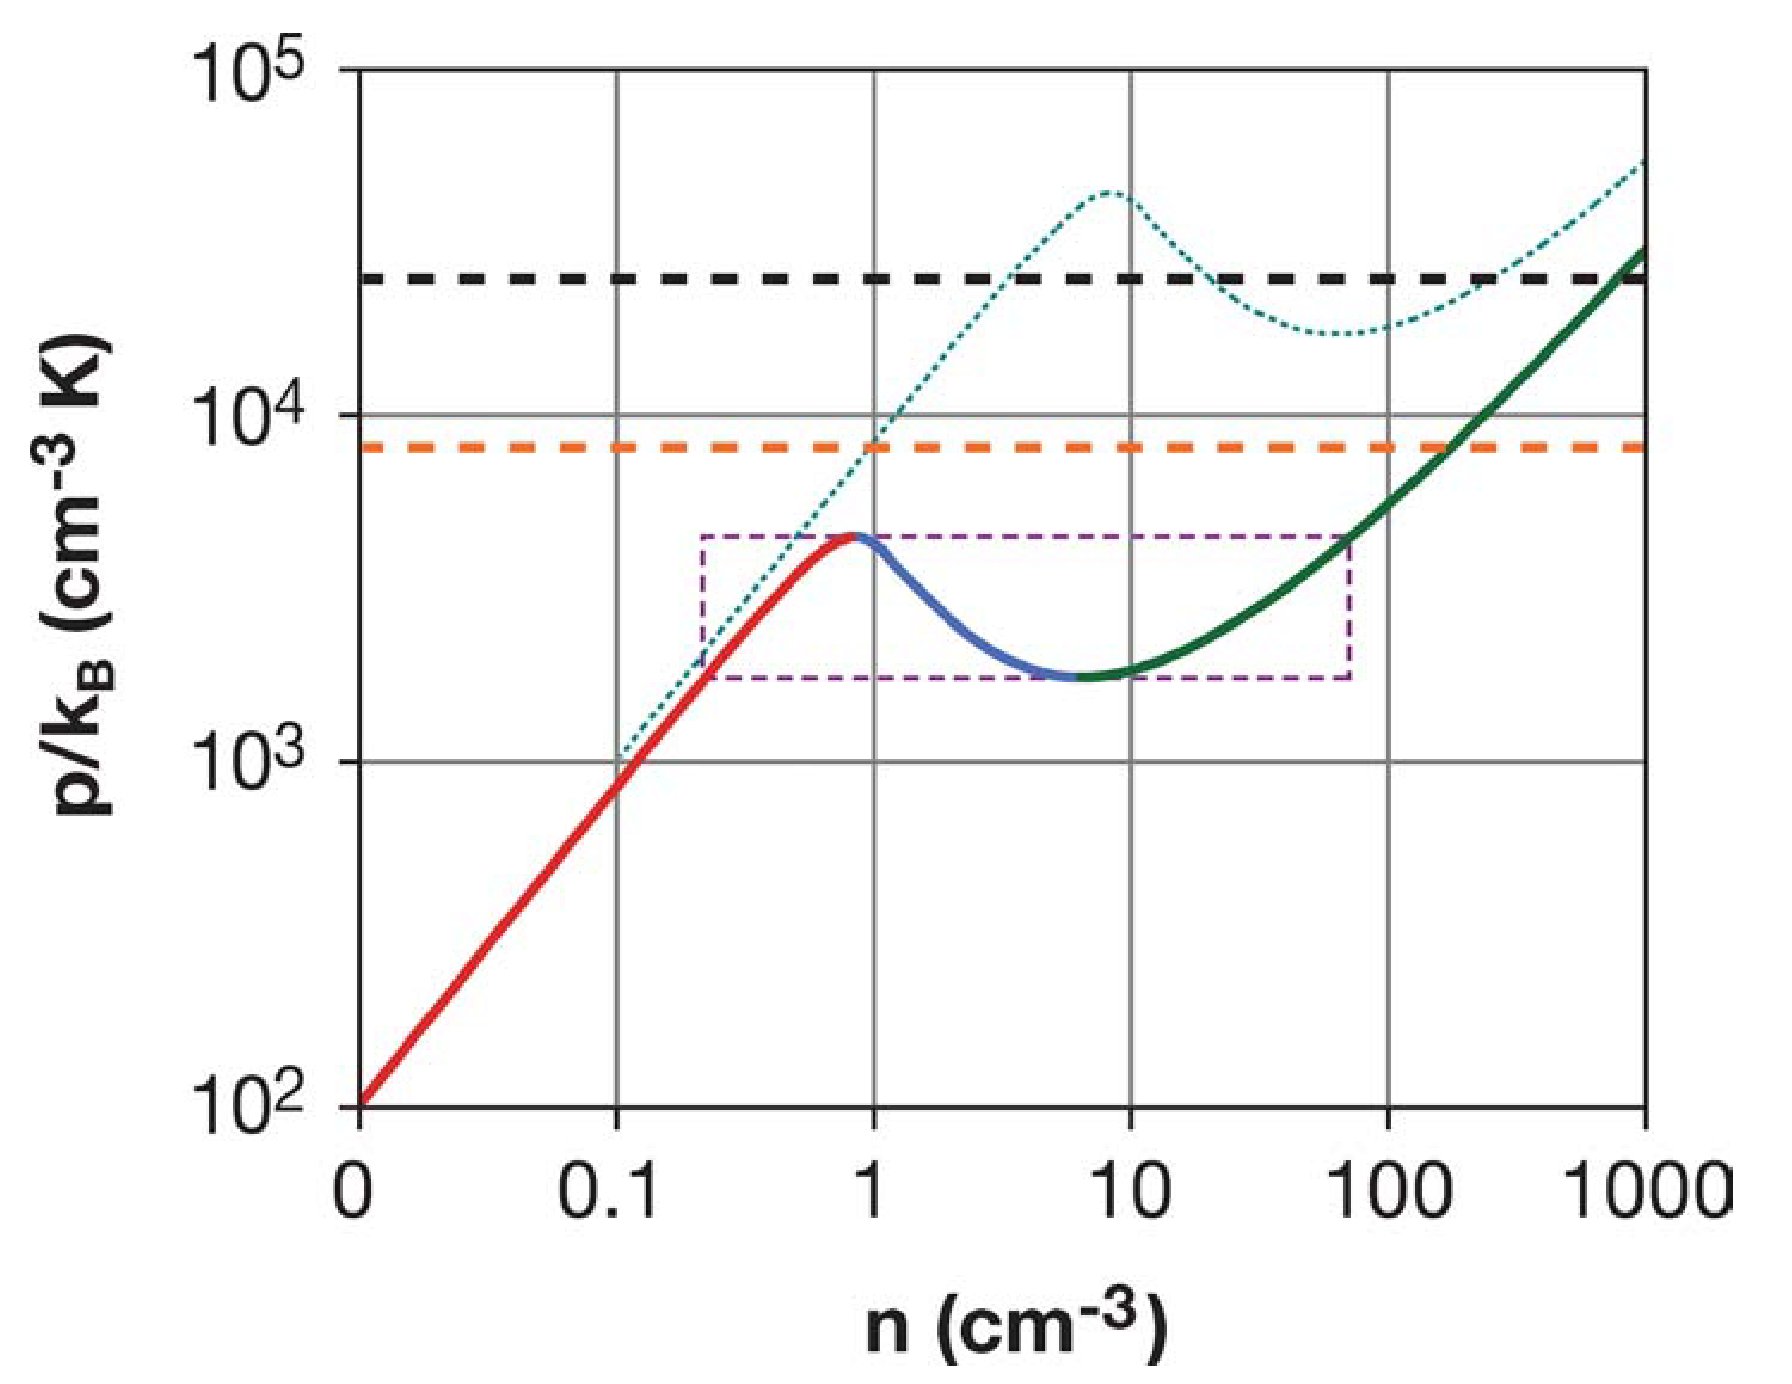
\includegraphics[width=10cm]{figures/pressure-density.png}}
\end{figure}

{\noindent}One of the most interesting features of $p(n)f$ is that over a density range of a factor of $350$, from $0.2$ to $70\,{\rm cm^{-3}}$, the thermal pressure variation is less than a factor of three. In Figure \ref{fig:pressure-density}, this region is shown enclosed by a dashed purple rectangle. It is a regime in which the thermal pressure offers essentially zero bulk modulus. This means that if, for some reason, the ISM had a totally random distribution of densities within this range, the corresponding distribution of thermal pressures would be observationally indistinguishable from one in which thermal pressure had an active role in arranging things, except there would be no range of forbidden densities. The small variation in thermal pressure between regions of differing density can be compensated by slight changes in the somewhat stronger magnetic field pressure. This is true when establishing pressure uniformity across the magnetic field lines, but equilibrium parallel to the field cannot be established in this way.

{\noindent}\textbf{Variance ($\nu_x~{\rm or}~\sigma^2$):} The second order statistical \textit{moment} which is a measure of the deviation from the \textit{mean}. The variance is defined as

\begin{align*}
    \mu_x = \frac{1}{N-1} \sum_{i=1}^N (x_i-\bar{x})
\end{align*}

{\noindent}and, like the \textit{mean}, has the same dimensions as $x_i$.

{\noindent}\textbf{Volume filling factor ($f$):} A correction factor such that a fraction $f$ of the line of sight intersects clouds of uniform density $N$. There are three effects of the interstellar magnetic field that conspire to lower the filling factor of hot cavities: (1) the background magnetic pressure acting on the surrounding shells directly opposes their expansion, (2) the magnetic tension in the swept-up field lines gives rise to an inward restoring force, while the associated magnetic pressure prevents the shells from fully collapsing and, therefore, keeps them relatively thick, and (3) the enhanced external ``signal speed'' causes the shells to merge earlier than they would in an unmagnetized medium.

{\noindent}\textbf{Warm ionized medium (WIM):} A diffuse phase of the \textit{interstellar medium} with a typical temperature of $T\sim8,000\,{\rm K}$ and average electron density of $\sim0.2-0.5\,{\rm cm^{-3}}$.  The ionized gas has mostly been mapped using the H$\alpha$ line. One limitation of the H$\alpha$ line comes from the obscuration caused by dust, which restricts visibility to within $2-3\,{\rm kpc}$ from the Sun. Using polarization gradients of \textit{synchrotron radiation}, it was shown by Gaensler (2011) that the turbulence of the WIM has a relatively low \textit{sonic Mach number}, $\mathcal{M}_s\lesssim2$.

{\noindent}\textbf{Warm neutral medium (WNM):} A thermally-stable phase of the atomic ISM with a typical density and kinetic temperature of $n\sim0.2-0.9\,{\rm cm^{-3}}$ and $T_K\sim5000-8300\,{\rm K}$, respectively.

{\noindent}\textbf{Warm partially ionized medium (WPIM):}

{\noindent}\textbf{Wave turbulence:}

{\noindent}\textbf{Zeeman effect:} The effect of a single spectral line splitting into multiple components in the presence of a static magnetic field due to the degeneracy between various electron energy levels that become broken when exposed to an external magnetic field. In an astrophysical context, a magnetic field produces small frequency shifts in the left- and right-handed circular polarized components of a given spectral line with respect to the intrinsic central frequency of the atom of molecule. Zeeman splitting is used to measure the parallel component of the magnetic field via atomic and molecular gas. The first measurement of an astrophysical magnetic field was using Zeeman splitting. The $21\,{\rm cm}$ line of atomic hydrogen is the most widespread, and it provides an opportunity to measure splitting in both emission and absorption. Zeeman splitting is a powerful tool as the magnetic field can be directly determined from the energy difference between the electron levels. The separation in energy of the magnetic hyperfine levels from the unsplit level of the zero magnetic field case is given by

\begin{align*}
    \Delta E = -\mu_Bm_FgB ~ [{\rm J}],
\end{align*}

{\noindent}where $\mu_B$ is the Bohr magneton, $m_F$ is the quantum number of the Zeeman splitting, $B$ is the magnetic field strength, and $g$ is the Land\'e g-factor. However, the effect is difficult to observe since the frequency shift ($\Delta\nu$) in the spectral lines is small:

\begin{align*}
    \Delta\nu = \frac{\mu_Bm_FgB}{h} ~ [{\rm Hz}].
\end{align*}

{\noindent}Such a frequency shift is usually smaller than the spectral linewidth, making Zeeman splitting observations resolution limited. Lower frequencies produce better Zeeman splitting results because, although the splitting is independent of the line frequency itself, the higher the frequency, the broader the linewidth.

{\noindent}The statistical sample of measured Zeeman splittings is woefully small and desperately needs to be expanded. Zeeman-splitting observations are time-consuming: typically tens of hours are required for each source. In addition, Zeeman splitting observations cannot be related to the large-scale GMF.

{\noindent}\textbf{Zenith:} The point in the sky or celestial sphere directly above an observer.

{\noindent}\textbf{Zeroth moment:} 








































%%%%%%%%%%%%%%%%%%%%%%%%
%                                                                       %
%                       VARIABLES                            %
%                                                                       %
%%%%%%%%%%%%%%%%%%%%%%%%

\newpage
\section{Variables}

{\noindent}\textbf{Alfv\'en Mach number}: $\mathcal{M}_A~[{\rm dimensionless}]$

{\noindent}\textbf{Alfv\'en speed}: $v_A~[{\rm m\,s^{-1}}]$

{\noindent}\textbf{Ambipolar diffusion scale}: $L_\mathrm{AD}~[{\rm m}]$

{\noindent}\textbf{Ambipolar diffusivity}: $\nu_\mathrm{AD}$

{\noindent}\textbf{Angle}: $\theta~[{\rm rad}]$

{\noindent}\textbf{Autocorrelation}: $C(\delta r)~[{\rm dimensionless}]$

{\noindent}\textbf{Bandwidth in frequency}: $\Delta\nu~[{\rm Hz}]$

{\noindent}\textbf{Bandwidth in wavelength}: $\Delta\lambda~[{\rm Hz}]$

{\noindent}\textbf{Bohr magneton}: $\mu_B$

{\noindent}$\boldsymbol{\beta}$ \textbf{parameter}: $\beta$

{\noindent}\textbf{Channel central frequency}: $\nu_c~[{\rm Hz}]$

{\noindent}\textbf{Channel width in frequency}: $\delta\nu~[{\rm Hz}]$

{\noindent}\textbf{Channel central wavelength}: $\lambda_c~[{\rm m}]$

{\noindent}\textbf{Channel width in wavelength}: $\delta\lambda~[{\rm m}]$

{\noindent}\textbf{Charge density}: $\rho_e~[{\rm C\,m^{-3}}]$

{\noindent}\textbf{Complex conjugate}: ${f(x)}^*\,{\rm or}\,\bar{f}(x)$

{\noindent}\textbf{Current density}: $\vec{j} ~ [{\rm A\,m^{-3}}]$

{\noindent}\textbf{Delta function}: $\delta (x)$

{\noindent}\textbf{Delta variance}: $\sigma_\Delta^2(L)$

{\noindent}\textbf{Density}: $\rho~[{\rm m^{-3}}]$

{\noindent}\textbf{Density of electrons}: $\rho_e~[{\rm m^{-3}}]$

{\noindent}\textbf{Density of ions}: $\rho_i~[{\rm m^{-3}}]$

{\noindent}\textbf{Density of neutrals}: $\rho_n~[{\rm m^{-3}}]$

{\noindent}\textbf{Diameter of window (RHT)}: $D_W ~ [{\rm pixels}]$

{\noindent}\textbf{Dirac delta function}: $\delta(x)$

{\noindent}\textbf{Dispersion measure}: ${\rm DM} ~ [{\rm pc\,cm^{-3}}]$

{\noindent}\textbf{Dust-to-gas mass ratio}: $r ~ [{\rm dimensionless}]$

{\noindent}\textbf{Dynamic viscosity}: $\mu ~ [{\rm Ps\,s}]$

{\noindent}\textbf{Electron charge}: $e~[{\rm C}]$

{\noindent}\textbf{Electron mass}: $e_m~[{\rm kg}]$

{\noindent}\textbf{Electron plasma pressure}: $P_e~[{\rm Pa}]$

{\noindent}\textbf{Electron temperature}: $T_e~[{\rm K}]$

{\noindent}\textbf{Emission cross section per H nucleon}: $\sigma_e(\nu) ~ [{\rm cm^2}]$

{\noindent}\textbf{Emission measure}: ${\rm EM} ~ [{\rm pc\,cm^{-6}}]$

{\noindent}\textbf{Emissivity index}: $\beta ~ [{\rm dimensionless}]$

{\noindent}\textbf{Energy spectrum}: $E(k)~[{\rm Jy\,m^{-1}}]$

{\noindent}\textbf{Expectation value of $\theta$ on any domain (RHT)}: $\langle\theta\rangle' ~ [{\rm rad}]$

{\noindent}\textbf{Expectation value of $\theta$ on $\theta\in[0,\pi)$ (RHT)}: $\langle\theta\rangle ~ [{\rm rad}]$

{\noindent}\textbf{Faraday depth}: $\phi~[{\rm rad\,m^{-2}}]$

{\noindent}\textbf{Faraday dispersion function (no spectral dependence)}: $F(\phi)~[{\rm rad\,m^{-2}}]$

{\noindent}\textbf{Faraday dispersion function (general form)}: $F(\phi,\lambda)~[{\rm rad\,m^{-2}}]$

{\noindent}\textbf{Frequency}: $\nu~[{\rm Hz}]$

{\noindent}\textbf{Frictional coupling coefficient between ions and neutrals}: $\alpha~[{\rm dimensionless}]$

{\noindent}\textbf{FWHM of RMTF main peak}: $\Delta\phi~[{\rm rad\,m^{-2}}]$

{\noindent}\textbf{Fourier transform (FT)}: $\hat{f}(x)$

{\noindent}\textbf{Hydrogen column density}: $N_{\rm H} ~ [{\rm cm^{-2}}]$

{\noindent}\textbf{HI column density}: $N_{\rm HI} ~ [{\rm cm^{-2}}]$

{\noindent}\textbf{HI density}: $n_{\rm HI}~[{\rm cm^{-3}}]$

{\noindent}\textbf{Incremental position}: $\delta r~[{\rm m}]$

{\noindent}\textbf{Intensity of thermal dust emission}: $I_\nu~ [{\rm W\,m^{-2}\,Hz^{-1}\,sr^{-1}}]$

{\noindent}\textbf{Intensity threshold}: $Z ~ [{\rm dimensionless}]$

{\noindent}\textbf{Jansky}: $\mathrm{Jy} ~ [\rm unit]$

{\noindent}\textbf{Joule}: $\mathrm{J} ~ [\rm unit]$

{\noindent}\textbf{Land\'e g-factor}: $g$

{\noindent}\textbf{Lorentz factor}: $\gamma ~ [\rm dimensionless]$

{\noindent}\textbf{Luminosity per H atom:} $L ~ [{\rm W\,H^{-1}}]$

{\noindent}\textbf{Mach number}: $\mathcal{M}~[{\rm dimensionless]}$

{\noindent}\textbf{Magnetic field}: $\vec{B}~[{\rm \mu G]}$

{\noindent}\textbf{Magnetic field strength (parallel component)}: $\lvert\vec{B}_\parallel\rvert~[{\rm \mu G]}$

{\noindent}\textbf{Magnetic field strength (tangential component)}: $\lvert\vec{B}_\perp\rvert~[{\rm \mu G]}$

{\noindent}\textbf{Magnetic field strength (total)}: $\lvert\vec{B}_{\rm tot}\rvert~[{\rm \mu G]}$

{\noindent}\textbf{Magnetic pressure}: $P_{\rm mag} ~ [{\rm Pa]}$

{\noindent}\textbf{Mass absorption coefficient:} $\kappa_\nu ~ [{\rm cm^2\,g^{-1}}]$

{\noindent}\textbf{Mean}: $\mu_x$

{\noindent}\textbf{Mean molecular weight:} $\mu ~ [{\rm dimensionless}]$

{\noindent}\textbf{Modified blackbody:} $I_\nu ~ [{\rm W\,m^{-2}\,Hz^{-1}\,sr^{-1}}]$

{\noindent}\textbf{Momentum diffusivity}: $\nu ~ [{\rm m^2\,s^{-1}}]$

{\noindent}\textbf{Number density}: $n ~ [{\rm m^{-3}}]$

{\noindent}\textbf{Number of $\theta$ bins (RHT)}: $n ~ [{\rm dimensionless}]$

{\noindent}\textbf{Optical depth}: $\tau_\nu~[{\rm dimensionless}]$

{\noindent}\textbf{Order}: $p~[{\rm dimensionless}]$

{\noindent}\textbf{Planck constant}: $h~[{\rm J\,s}]$

{\noindent}\textbf{Planck constant (reduced)}: $\hbar~[{\rm J\,s}]$

{\noindent}\textbf{Planck function}: $B_\nu(T)~[{\rm W\,m^{-2}\,Hz^{-1}\,sr^{-1}}]~{\rm or}~B_\lambda(T)~[{\rm W\,m^{-2}\,m^{-1}\,sr^{-1}}]$

{\noindent}\textbf{Plasma beta}: $\beta_{\rm th} ~ [{\rm dimensionless}]$

{\noindent}\textbf{Polarization angle}: $\chi~[{\rm rad}]$

{\noindent}\textbf{Polarization angle (RHT)}: $\chi_\mathrm{RHT} ~ [{\rm rad}]$

{\noindent}\textbf{Polarization angle at $\lambda=0$}: $\chi_0~[{\rm rad}]$

{\noindent}\textbf{Polarization fraction}: $p(\lambda^2)~[{\rm dimensionless}]$

{\noindent}\textbf{Polarization gradient}: $\left\lvert\dfrac{\partial\vec{P}}{\partial s}\right\rvert~{\rm or}~\lvert\vec\nabla\vec{P}\rvert ~ [\rm Jy\,beam^{-1}]$

{\noindent}\textbf{Polarization gradient (maximum value)}: $\left\lvert\dfrac{\partial\vec{P}}{\partial s}\right\rvert_{\rm max}~{\rm or}~\lvert\vec\nabla\vec{P}\rvert_{\rm max} ~ [\rm Jy\,beam^{-1}]$

{\noindent}\textbf{Polarization gradient (radial component; maximum value)}: $\left\lvert\dfrac{\partial\vec{P}}{\partial s}\right\rvert_\mathrm{rad}~ [\rm Jy\,beam^{-1}]$

{\noindent}\textbf{Polarization gradient (tangential component; maximum value)}: $\left\lvert\dfrac{\partial\vec{P}}{\partial s}\right\rvert_\mathrm{tan}~ [\rm Jy\,beam^{-1}]$

{\noindent}\textbf{Polarization gradient (direction)}: $\mathrm{arg}(\vec\nabla\vec{P}) ~ [\rm rad]$

{\noindent}\textbf{Polarized intensity}: $P ~ [\rm Jy]$

{\noindent}\textbf{Polarized intensity error}: $\sigma_P ~ [\rm Jy]$

{\noindent}\textbf{Polarized intensity (observed)}: $\hat{P} ~ [\rm Jy]$

{\noindent}\textbf{Polarized intensity (true)}: $P_T ~ [\rm Jy]$

{\noindent}\textbf{Polarized surface brightness}: $P(\lambda^2) ~ [\rm Jy]$

{\noindent}\textbf{Polarized surface brightness (observed)}: $\tilde{P}(\lambda^2) ~ [\rm Jy]$

{\noindent}\textbf{Position}: $r~[{\rm m}]$

{\noindent}\textbf{Power spectrum}: $P(k)$

{\noindent}\textbf{Quantum number of Zeeman splitting}: $m_F$

{\noindent}\textbf{Radial component of polarization gradient}: $\dfrac{\partial\mathbf{P}}{\partial s}_\mathrm{rad} ~ [{\rm Jy\,pc^{-1}}]$

{\noindent}\textbf{Rayleigh}: ${\rm R} ~ [{\rm unit}]$

{\noindent}\textbf{Redshift}: $z ~ [{\rm dimensionless}]$

{\noindent}\textbf{Resistivity}: $\eta~[{\rm \Omega\,m}]$

{\noindent}\textbf{Rest mass}: $m_0~[{\rm kg}]$

{\noindent}\textbf{Reynolds number}: ${\rm Re}~[{\rm dimensionless}]$

{\noindent}\textbf{Reynolds number for ambipolar diffusion}: ${\rm R}_\mathrm{\rm AD}~[{\rm dimensionless}]$

{\noindent}\textbf{RHT angle}: $\theta~[{\rm rad}]$

{\noindent}\textbf{RHT backprojection}: $R(x,y) ~ [{\rm dimensionless}]$

{\noindent}\textbf{RHT backprojection sampling disk around star}: $R_*(x,y) ~ [{\rm dimensionless}]$

{\noindent}\textbf{RHT distance}: $\rho~[{\rm pixels}]$

{\noindent}\textbf{RHT intensity vs angle}: $R(\theta,x_0,y_0)~[{\rm dimensionless}]$

{\noindent}\textbf{Rotation measure}: ${\rm RM~[rad\,m^{-2}]}$

{\noindent}\textbf{Rotation measure transfer function (RMTF)}: $R(\phi) {\rm [rad\,m^{-2}]}$

{\noindent}\textbf{Sonic Mach number}: $\mathcal{M}_s~[{\rm dimensionless]}$

{\noindent}\textbf{Sound speed}: $c_s ~ [{\rm m\,s^{-1}}]$

{\noindent}\textbf{Specific heat}: $c_p ~ [{\rm J\,kg^{-1}\,K}]$

{\noindent}\textbf{Spectral correlation function}: $S_{x,y}~[\rm{dimensionless}]$

{\noindent}\textbf{Spectral index}: $\alpha~[\rm{dimensionless}]$

{\noindent}\textbf{Spectral irradiance:} $E_\nu(T)~[{\rm W\,m^{-2}\,Hz^{-1}}]~{\rm or}~E_\lambda(T)~[{\rm W\,m^{-2}\,m^{-1}}]$

{\noindent}\textbf{Speed of light}: $c~[\rm{m\,s^{-1}}]$

{\noindent}\textbf{Standard deviation}: $\sigma(x)$

{\noindent}\textbf{Stokes I}: $I ~ [\rm Jy]$

{\noindent}\textbf{Stokes I error}: $\sigma_I ~ [\rm Jy]$

{\noindent}\textbf{Stokes Q}: $Q ~ [\rm Jy]$

{\noindent}\textbf{Stokes Q error}: $\sigma_Q ~ [\rm Jy]$

{\noindent}\textbf{Stokes Q (true)}: $Q_T ~ [\rm Jy]$

{\noindent}\textbf{Stokes Q (observed)}: $\hat{Q} ~ [\rm Jy]$

{\noindent}\textbf{Stokes Q (RHT)}: $Q_\mathrm{RHT} ~ [\rm Jy]$

{\noindent}\textbf{Stokes U}: $U ~ [\rm Jy]$

{\noindent}\textbf{Stokes U error}: $\sigma_U ~ [\rm Jy]$

{\noindent}\textbf{Stokes U (true)}: $U_T ~ [\rm Jy]$

{\noindent}\textbf{Stokes U (observed)}: $\hat{U} ~ [\rm Jy]$

{\noindent}\textbf{Stokes U (RHT)}: $U_\mathrm{RHT} ~ [\rm Jy]$

{\noindent}\textbf{Stokes V}: $V ~ [\rm Jy]$

{\noindent}\textbf{Structure function}: $S_p$

{\noindent}\textbf{Structure function power-law slope}: $\zeta_p$

{\noindent}\textbf{Tangential component of polarization gradient}: $\dfrac{\partial\mathbf{P}}{\partial s}_\mathrm{tan} ~ [{\rm Jy\,pc^{-1}}]$

{\noindent}\textbf{Thermal conductivity}: $k ~ [{\rm W\,m^{-1}\,K}]$

{\noindent}\textbf{Thermal diffusivity}: $\alpha ~ [{\rm m^2\,s^{-1}}]$

{\noindent}\textbf{Thermal electron density}: $n_e~[{\rm cm^{-3}}]$

{\noindent}\textbf{Thermal electron fraction}: $x_e ~ [{\rm dimensionless}]$

{\noindent}\textbf{Thermal pressure}: $P_{\rm th} ~ [{\rm Pa}]$

{\noindent}\textbf{Thermal pressure (ionized)}: $P_{\rm th,i} ~ [{\rm Pa}]$

{\noindent}\textbf{Thermal pressure (neutral)}: $P_{\rm th,n} ~ [{\rm Pa}]$

{\noindent}\textbf{Variance}: $\nu_x~{\rm or}~\sigma^2$

{\noindent}\textbf{Velocity}: $\vec{v} ~ [{\rm m\,s^{-1}}]$

{\noindent}\textbf{Viscosity coefficient}: $\mu ~ [{\rm Pa\,s}]$

{\noindent}\textbf{Wavelength}: $\lambda~[{\rm m}]$

{\noindent}\textbf{Wavelength to which all polarization vectors are de-rotated}: $\lambda_0~[{\rm m}]$

{\noindent}\textbf{Wavenumber}: $k~[{\rm m^{-1}}]$

{\noindent}\textbf{Weight function}: $W(\lambda^2)~[\rm{dimensionless}]$

{\noindent}\textbf{Zeeman splitting energy difference}: $\Delta E ~ [{\rm J}]$

{\noindent}\textbf{Zeeman splitting frequency difference}: $\Delta \nu ~ [{\rm Hz}]$








































%%%%%%%%%%%%%%%%%%%%
%                                                          %
%                      EQUATIONS               %
%                                                          %
%%%%%%%%%%%%%%%%%%%%

\newpage
\section{Equations}

{\noindent}\textbf{Alfv\'en Mach number:}
\begin{align*}
    \mathcal{M}_A = \left\langle\frac{\lvert\vec{v}\rvert}{v_A}\right\rangle ~ [{\rm dimensionless}]
\end{align*}

{\noindent}\textbf{Alfv\'en speed:}
\begin{align*}
    v_A = \frac{\lvert\vec{B}\lvert}{\sqrt{\rho}} ~ [{\rm m\,s^{-1}}]
\end{align*}

{\noindent}\textbf{Ambipolar diffusion scale:}
\begin{align*}
    L_\mathrm{AD} = \dfrac{V_A}{\alpha\rho_i} ~ [\rm m]
\end{align*}

{\noindent}\textbf{Ambipolar diffusivity:}
\begin{align*}
    \nu_\mathrm{AD} = \dfrac{B^2}{4\pi\rho_i\rho_n\alpha} ~ [{\rm m^s\,s^{-1}}]
\end{align*}

{\noindent}\textbf{Autocorrelation:}
\begin{align*}
    C(\delta r) = \langle f(r)f(r+\delta r)\rangle ~ [{\rm dimensionless}]
\end{align*}

{\noindent}$\beta$ \textbf{parameter}: 
\begin{align*}
    \beta \equiv \frac{c_s^2}{v_A^2} ~ [{\rm dimensionless}]
\end{align*}

{\noindent}\textbf{Channel central wavelength:} 
\begin{align*}
\lambda_c^2 \approx \dfrac{c^2}{\nu_c^2} \left(1+\dfrac{3}{4}\left(\dfrac{\delta\nu}{\nu_c}\right)^2\right) ~ [{\rm m^2}]
\end{align*}
(Brentjens \& de Bruyn, 2005)

{\noindent}\textbf{Charge conservation:} 
\begin{align*}
    \frac{\partial\rho_e}{\partial t} + \vec\nabla\cdot\vec{j} = 0
\end{align*}

{\noindent}\textbf{Channel width in wavelength:} 
\begin{align*}
\delta\lambda^2 \approx \dfrac{2c^2\delta\nu}{\nu_c^3} \left(1+\dfrac{1}{2}\left(\dfrac{\delta\nu}{\nu_c}\right)^2\right) ~ [{\rm m^2}]
\end{align*}
(Brentjens \& de Bruyn, 2005)

{\noindent}\textbf{Current density}:
\begin{align*}
    \vec{j} = c\nabla\times\frac{\vec{B}}{4\pi} ~ [{\rm A\,m^{-2}}]
\end{align*}
(Schoeffler et al., 2016)

{\noindent}\textbf{Delta variance:}
\begin{align*}
    \sigma_\Delta^2(L) = \left\langle \int\limits_0^{3L/2} {(A[r+x]-\langle A\rangle)\odot(x)}^2\mathrm{d}x \right\rangle,
\end{align*}

{\noindent}\textbf{Dispersion measure (DM):}
\begin{align*}
    {\rm DM} = -\int\limits_\mathrm{source}^\mathrm{observer} n_e\vec{{\rm d}\ell} ~ [{\rm pc\,cm^{-3}}]
\end{align*}

{\noindent}\textbf{Electron plasma pressure}:
\begin{align*}
    P_e = T_e \eta ~ [{\rm Pa}]
\end{align*}
(Schoeffler et al., 2016)

{\noindent}\textbf{Electron temperature}:
\begin{align*}
    T_e = \frac{P_e}{\eta} ~ [{\rm K}]
\end{align*}
(Schoeffler et al., 2016)

{\noindent}\textbf{Emission cross section per H nucleon}:
\begin{align*}
    \sigma_e(\nu) = \frac{\tau_\nu}{N_{\rm H}} ~ [{\rm cm^2}]
\end{align*}
(Roy et al., 2013)

{\noindent}\textbf{Emission measure:}
\begin{align*}
    {\rm EM} &= -\int\limits_\mathrm{source}^\mathrm{observer} n_e^2\vec{{\rm d}\ell} ~ [{\rm pc\,cm^{-6}}] \\
    {\rm EM}(I_{\rm H\alpha}) &= 2.75 \left(\frac{T_e}{10^4\,{\rm K}}\right)^{0.9} \left(\frac{I_{\rm H\alpha}}{R}\right) e^\tau ~ [{\rm pc\,cm^{-6}}]
\end{align*}
(Reynolds 1988)

{\noindent}\textbf{Expectation value of $\theta$ on any domain (RHT):}
\begin{align*}
    \langle\theta\rangle' = \frac{1}{2}\arctan \left[\frac{\int\sin(2\theta)R_*(\theta)\mathrm{d}\theta}{\int\cos(2\theta)R_*(\theta)\mathrm{d}\theta}\right]
\end{align*}

{\noindent}\textbf{Expectation value of $\theta$ on $\theta\in[0,\pi)$ (RHT):}
\begin{align*}
    \langle\theta\rangle = \pi - {\rm mod}(\langle\theta\rangle'+\pi,\pi) ~ [{\rm rad}]
\end{align*}

{\noindent}\textbf{Faraday depth:} 
\begin{align*}
    \phi(\vec{r}) = -0.81 \int\limits_\mathrm{source}^\mathrm{observer}n_e\vec{B}\cdot\vec{{\rm d}r} ~ [{\rm rad\,m^{-2}}]
\end{align*}

{\noindent}\textbf{Faraday depth standard error:}
\begin{align*}
\sigma_\phi &= \left[ \dfrac{1}{N-2} \dfrac{\sum_i\chi_i^2}{\sum_i(\lambda_i^2)^2 - N^{-1}(\sum_i\lambda_i^2)^2} \right]^{-1} \\
&= \left[ \dfrac{1}{N-2} \dfrac{(N-1)(\sigma_\chi^2 + \cancel{\langle\chi\rangle})}{\sum_i(\lambda_i^2)^2 - N^{-1}(\sum_i\lambda_i^2)^2} \right]^{-1} \\
&= \left[ \dfrac{N-1}{N-2} \dfrac{\sigma_\chi^2}{\sum_i(\lambda_i^2)^2 - N^{-1}(\sum_i\lambda_i^2)^2} \right]^{-1} \\
&\approx \left[ \dfrac{\sigma_Q^2\approx\sigma_U^2\approx\sigma^2}{4(N-2)\lvert\lvert P \rvert\rvert^2\sigma_{\lambda^2}^2} \right]^{-1} ~ [{\rm rad\,m^{-2}}]
\end{align*}
(Brentjens \& de Bruyn, 2005)

{\noindent}\textbf{Faraday dispersion function:}
\begin{align*}
F(\phi) = \int\limits_{\infty}^\infty P(\lambda^2)\mathrm{e}^{-2i\phi\lambda^2}\mathrm{d}\lambda^2 ~ [{\rm rad\,m^{-2}}]
\end{align*}

{\noindent}\textbf{Faraday dispersion function (reconstructed):}
\begin{align*}
\tilde{F}(\phi) \equiv \dfrac{\int\limits_{-\infty}^\infty \tilde{P}(\lambda^2)\mathrm{e}^{-2i\phi(\lambda^2-\lambda_0^2)}\mathrm{d}\lambda^2}{\int\limits_{-\infty}^\infty W(\lambda^2)\mathrm{d}\lambda^2} = F(\phi) * R(\phi) ~ [{\rm rad\,m^{-2}}]
\end{align*}

{\noindent}\textbf{Fourier transform (FT):}
\begin{align*}
    \hat{f}(x) = \int\limits_{-\infty}^\infty f(x')e^{-2\pi xx'}dx'
\end{align*}

{\noindent}\textbf{Hydrogen column density}:
\begin{align*}
    N_{\rm H} = (11.5\pm0.5)\times10^{21}\,E({\rm J-K_s}) ~ [{\rm cm^{-2}}]~(N_{\rm H}\lesssim5\times10^{21}\,{\rm cm^{-2}})
\end{align*}
(Martin et al., 2012)

{\noindent}\textbf{Induction equation:}
\begin{align*}
    \frac{\partial\vec{B}}{\partial t} = \nabla\times(\vec{v}\times\vec{B}) + \frac{\eta c^2}{4\pi}\nabla^2\vec{B} - \frac{1}{en}\nabla\times(\vec{j}\times\vec{B}) - \frac{c}{ne}\nabla n\times\nabla T_e
\end{align*}
(Schoeffler et al., 2016)

{\noindent}\textbf{Intensity of thermal dust emission}:
\begin{align*}
    I_\nu &= \tau_\nu B_\nu(T) ~ [{\rm W\,m^{-2}\,Hz^{-1}\,sr^{-1}}] \\
             &\equiv \sigma_e(\nu)N_{\rm H}B_\nu(T) ~ [{\rm W\,m^{-2}\,Hz^{-1}\,sr^{-1}}] \\
             &= r\mu m_{\rm H}N_{\rm H}\kappa_\nu B_\nu(T) ~ [{\rm W\,m^{-2}\,Hz^{-1}\,sr^{-1}}]
\end{align*}

{\noindent}\textbf{Inverse Fourier transform (FT):}
\begin{align*}
    f(x) = \int\limits_{-\infty}^\infty \hat{f}(x')e^{2\pi ixx'}dx'
\end{align*}

{\noindent}\textbf{Kurtosis:}
\begin{align*}
    \beta_x = \frac{1}{N} \sum_{i=1}^N \left(\frac{x_i-\mu_x}{\sigma}\right)^3 ~ [{\rm dimensionless}]
\end{align*}

{\noindent}\textbf{Lorentz factor:}
\begin{align*}
    \gamma = \sqrt{\frac{1 - (v/c)^2}{c^2}} ~ [{\rm dimensionless}]
\end{align*}

{\noindent}\textbf{Luminosity per H atom:}
\begin{align*}
    L = \int 4\pi\kappa_0(\nu/\nu_0)^\beta \mu m_{\rm H}B_\nu(T) \,{\rm d}\nu ~ [{\rm W\,H^{-1}}]
\end{align*}

{\noindent}\textbf{Magnetic field strength (parallel component)}:
\begin{align*}
    \lvert\vec{B}_\parallel\rvert = \frac{\rm RM}{0.81\sqrt{\rm EM}\sqrt{fL}} ~[{\rm \mu G]}
\end{align*}

{\noindent}\textbf{Magnetic field strength (total)}:
\begin{align*}
    \lvert\vec{B}_{\rm tot}\rvert = \sqrt{3}\lvert\vec{B}_\parallel\rvert ~[{\rm \mu G]}
\end{align*}

{\noindent}\textbf{Magnetic pressure}:
\begin{align*}
    P_{\rm mag} = \frac{\lvert\vec{B_{\rm tot}}\rvert^2}{8\pi}~ [{\rm Pa]}
\end{align*}

{\noindent}\textbf{Magnetohydrodynamic (MHD) equations:}

\begin{align*}
    \vec\nabla\cdot\vec{B} &= 0 \\
    \vec\nabla\cdot\vec{E} &= 4\pi\rho_e \\
    c\vec\nabla\times\vec{E} &= - \frac{\partial\vec{B}}{\partial t} \\
    c\vec\nabla\times\vec{B} &= 4\pi\vec{j} + \frac{\partial\vec{E}}{\partial t}
\end{align*}

{\noindent}\textbf{Mass absorption coefficient:}
\begin{align*}
    \kappa_\nu &= \kappa_0 \left(\frac{\nu}{\nu_0}\right)^\beta ~ [{\rm cm^2\,g^{-1}}] \\
                       &= \frac{\sigma_e(\nu)}{\mu m_{\rm H}} ~ [{\rm cm^2\,g^{-1}}]
\end{align*}

{\noindent}\textbf{Mean:} 
\begin{align*}
    \mu_x = \frac{1}{N} \sum_{i=1}^N x_i
\end{align*}

{\noindent}\textbf{Modified blackbody:}
\begin{align*}
    I_\nu = \tau B_\nu(T) \left(\frac{\nu}{\nu_0}\right)^\beta ~ [{\rm W\,m^{-2}\,Hz^{-1}\,sr^{-1}}]
\end{align*}

{\noindent}\textbf{Number of $\theta$ bins (RHT):}
\begin{align*}
    n_\theta = \left[\pi\frac{\sqrt{2}}{2}(D_W-1)\right] ~ [{\rm dimensionless}]
\end{align*}

{\noindent}\textbf{Optical depth}:
\begin{align*}
    \tau_\nu = 3.28\times10^{-7} \left(\frac{T_e}{10^4\,{\rm K}}\right)^{-1.35} \left(\frac{\nu}{\rm GHz}\right)^{-2.1} \left(\frac{\rm EM}{\rm pc\,cm^{-6}}\right)
\end{align*}
(Oster 1961)

{\noindent}\textbf{Planck function:}
\begin{align*}
    B_\nu(T) = \left(\frac{2h\nu^3}{c^2}\right) \frac{1}{e^{h\nu/k_BT}-1} ~ [{\rm W\,m^{-2}\,Hz^{-1}\,sr^{-1}}] \\
    B_\lambda(T) = \left(\frac{2hc^2}{\lambda^5}\right) \frac{1}{e^{hc/\lambda k_BT}-1} ~ [{\rm W\,m^{-2}\,m^{-1}\,sr^{-1}}]
\end{align*}

{\noindent}\textbf{Plasma beta:} 
\begin{align*}
\beta_{\rm th} &= \frac{P_{\rm th}}{P_{\rm mag}} ~ [{\rm dimensionless}]\\
                      &= \frac{ \langle P_{\rm th,i}\rangle + \langle P_{\rm th,n}\rangle }{(B_{\rm tot}^2/8\pi)} ~ [{\rm dimensionless}] \\
                      &= \frac{2\langle n_e\rangle k_BT_i + \langle n_{\rm H}\rangle k_BT_n}{(B_{\rm tot}^2/8\pi)}  ~ [{\rm dimensionless}] \\
                      &= \frac{2f_en_e+ \langle n_{\rm H}\rangle k_BT_n}{(B_{\rm tot}^2/8\pi)}  ~ [{\rm dimensionless}]
                      &= \frac{2M_A^2}{M_S^2} ~ [{\rm dimensionless}]
\end{align*}

{\noindent}\textbf{Polarization angle:}
\begin{align*}
\chi &= \dfrac{1}{2}\arctan\left(\dfrac{U}{Q}\right) ~ [{\rm rad}] \\
&= \chi_0 + \mathrm{RM}\lambda^2 ~ [{\rm rad}]
\end{align*}

{\noindent}\textbf{Polarization angle (RHT):}
\begin{align*}
\chi_\mathrm{RHT} = \dfrac{1}{2}\arctan\left(\dfrac{U_\mathrm{RHT}}{Q_\mathrm{RHT}}\right) ~ [{\rm rad}]
\end{align*}

{\noindent}\textbf{Polarization angle distribution standard error:} 
\begin{align*}
\sigma_\chi = \left[ \dfrac{1}{N-1} \sum_i\chi_i^2 - \langle\chi\rangle \right]^{-1} ~ [{\rm rad}]
\end{align*}
(Brentjens \& de Bruyn, 2005)

{\noindent}\textbf{Polarization angle standard error:}
\begin{align*}
\sigma_\chi &= \sqrt{ \left(\dfrac{\partial\chi}{\partial Q}\right)^2\sigma_Q^2 + \left(\dfrac{\partial\chi}{\partial U}\right)^2\sigma_U^2 }\\
&= \sqrt{ \left(\dfrac{\partial\frac{1}{2}\arctan\frac{U}{Q}}{\partial Q}\right)^2\sigma_Q^2 + \left(\dfrac{\partial\frac{1}{2}\arctan\frac{U}{Q}}{\partial U}\right)^2\sigma_U^2 } \\
&= \sqrt{ \left(\dfrac{1}{4}\dfrac{U^2}{(Q^2+U^2)^2}\right)\sigma_Q^2 + \left(\dfrac{1}{4}\dfrac{Q^2}{(Q^2+U^2)^2}\right)\sigma_U^2 } \\
&= \dfrac{U^2\sigma_Q^2 + Q^2\sigma_U^2}{4\lvert\lvert P \rvert\rvert^4} ~ [{\rm rad}]
\end{align*}
(Brentjens \& de Bruyn, 2005)

{\noindent}\textbf{Polarization angle at $\lambda=0$ standard error:} 
\begin{align*}
\sigma_{\chi_0} = \left[ \dfrac{\sigma_Q^2\approx\sigma_U^2\approx\sigma^2}{4(N-2)\lvert\lvert P \rvert\rvert^2} \left( \dfrac{N-1}{N} + \dfrac{\lambda_0^4}{\sigma_{\lambda^2}^2} \right) \right]^{-1} ~ [{\rm rad}]
\end{align*}
(Brentjens \& de Bruyn, 2005)

{\noindent}\textbf{Polarization gradient}:
\begin{align*}
	\left\lvert\dfrac{\partial\vec{P}}{\partial s}\right\rvert = \sqrt{ \cos^2\theta\left(\left(\frac{\partial Q}{\partial x}\right)^2+\left(\frac{\partial U}{\partial x}\right)^2\right) + 2\cos\theta\sin\theta\left(\frac{\partial Q}{\partial x}\frac{\partial Q}{\partial y} + \frac{\partial U}{\partial x}\frac{\partial U}{\partial y}\right) + \sin^2\theta\left(\left(\frac{\partial Q}{\partial y}\right)^2 + \left(\frac{\partial U}{\partial y}\right)^2\right) } ~ [\rm Jy\,beam^{-1}]
\end{align*}
(Herron, 2005)

{\noindent}\textbf{Polarization gradient (direction):}
\begin{align*}
    \mathrm{arg}(\vec\nabla\vec{P}) \equiv \arctan \left[ \mathrm{sign} \left(\dfrac{\partial Q}{\partial x}\dfrac{\partial Q}{\partial y} + \dfrac{\partial U}{\partial x}\dfrac{\partial U}{\partial y}\right) \dfrac{\sqrt{\left(\dfrac{\partial Q}{\partial y}\right)^2 + \left(\dfrac{\partial U}{\partial y}\right)^2}}{\sqrt{\left(\dfrac{\partial Q}{\partial x}\right)^2 + \left(\dfrac{\partial U}{\partial x}\right)^2}} \right] ~ [\rm rad]
\end{align*}
(Herron, 2005)

{\noindent}\textbf{Polarization gradient (maximum value)}:
\begin{equation*}
\begin{split}
\left\lvert\dfrac{\partial\vec{P}}{\partial s}\right\rvert_\mathrm{max} = \sqrt{ \frac{1}{2}\left[ \left(\frac{\partial Q}{\partial x}\right)^2 + \left(\frac{\partial U}{\partial x}\right)^2 + \left(\frac{\partial U}{\partial x}\right)^2 + \left(\frac{\partial U}{\partial y}\right)^2 \right] + \frac{1}{2} 
  \sqrt{
    \begin{aligned}
    & \left[ \left(\frac{\partial Q}{\partial x}\right)^2 + \left(\frac{\partial U}{\partial x}\right)^2 + \left(\frac{\partial U}{\partial x}\right)^2 + \left(\frac{\partial U}{\partial y}\right)^2 \right]^2 \\
    &- 4\left[ \frac{\partial Q}{\partial x}\frac{\partial U}{\partial y} - \frac{\partial Q}{\partial y}\frac{\partial U}{\partial x}  \right]^2
    \end{aligned}
    }}
\end{split}
\end{equation*}
(Herron, 2005)

{\noindent}\textbf{Polarization gradient (radial component)}:
\begin{align*}
	\left\lvert\dfrac{\partial\vec{P}}{\partial s}\right\rvert_\mathrm{rad} = \cos\left(\arctan\frac{U}{Q}\right)\left(\frac{\partial Q}{\partial x}\cos\theta+\frac{\partial Q}{\partial y}\sin\theta\right) + \sin\left(\arctan\frac{U}{Q}\right)\left(\frac{\partial U}{\partial x}\cos\theta+\frac{\partial U}{\partial y}\sin\theta\right) ~ [\rm Jy\,beam^{-1}]
\end{align*}
(Herron, 2005)

{\noindent}\textbf{Polarization gradient (radial component; maximum value)}:
\begin{align*}
	\left\lvert\dfrac{\partial\vec{P}}{\partial s}\right\rvert_\mathrm{rad,max} = \sqrt{\frac{\left(Q\frac{\partial Q}{\partial x}+U\frac{\partial U}{\partial x}\right)^2 +\left(Q\frac{\partial Q}{\partial y}+U\frac{\partial U}{\partial y}\right)^2}{Q^2+U^2}} ~ [\rm Jy\,beam^{-1}]
\end{align*}
(Herron, 2005)

{\noindent}\textbf{Polarization gradient (tangential component)}:
\begin{align*}
	\left\lvert\dfrac{\partial\vec{P}}{\partial s}\right\rvert_\mathrm{tan} = -\sin\left(\arctan\frac{U}{Q}\right)\left(\frac{\partial Q}{\partial x}\cos\theta+\frac{\partial Q}{\partial y}\sin\theta\right) + \cos\left(\arctan\frac{U}{Q}\right)\left(\frac{\partial U}{\partial x}\cos\theta+\frac{\partial U}{\partial y}\sin\theta\right) ~ [\rm Jy\,beam^{-1}]
\end{align*}
(Herron, 2005)

{\noindent}\textbf{Polarization gradient (tangential component; maximum value)}:
\begin{align*}
	\left\lvert\dfrac{\partial\vec{P}}{\partial s}\right\rvert_\mathrm{tan,max} = \sqrt{\frac{\left(Q\frac{\partial U}{\partial x}-U\frac{\partial Q}{\partial x}\right)^2 +\left(Q\frac{\partial U}{\partial y}-U\frac{\partial Q}{\partial y}\right)^2}{Q^2+U^2}} ~ [\rm Jy\,beam^{-1}]
\end{align*}
(Herron, 2005)

{\noindent}\textbf{Polarization fraction:}
\begin{align*}
p(\lambda^2) = \dfrac{P(\lambda^2)}{I(\lambda^2)} ~ [{\rm dimensionless}]
\end{align*}

{\noindent}\textbf{Polarized intensity:}
\begin{align*}
    P\equiv\sqrt{Q^2+U^2} ~ [\rm Jy]
\end{align*}

{\noindent}\textbf{Polarized intensity (observed)}:
\begin{align*}
    \hat{P} &= \sqrt{\hat{Q}^2+\hat{U}^2} ~ [\rm Jy] \\
                &= \sqrt{(Q_T+\sigma_Q)^2+(U_T+\sigma_U)^2} ~ [\rm Jy]
\end{align*}

{\noindent}\textbf{Polarized intensity standard error:}
\begin{align*}
\sigma_P &= \sqrt{ \left(\dfrac{\partial\lvert\lvert P \rvert\rvert}{\partial Q}\right)^2\sigma_Q^2 + \left(\dfrac{\partial\lvert\lvert P \rvert\rvert}{\partial U}\right)^2\sigma_U^2 } \\
&= \sqrt{ \left(\dfrac{Q^2}{Q^2+U^2}\right)\sigma_Q^2 + \left(\dfrac{U^2}{Q^2+U^2}\right)\sigma_U^2 } \\
&= \sqrt{ \dfrac{Q^2}{\lvert\lvert P \rvert\rvert^2}\sigma_Q^2 + \dfrac{U^2}{\lvert\lvert P \rvert\rvert^2}\sigma_U^2 } ~ [\rm Jy]
\end{align*}
(Brentjens \& de Bruyn, 2005)

{\noindent}\textbf{Polarized surface brightness:}
\begin{align*}
P(\lambda^2) &= \lvert\lvert p(\lambda^2) \rvert\rvert I\mathrm{e}^{2i\chi} = p(\lambda^2)I(\lambda^2) = Q+iU ~ [\rm Jy] \\
&= \int\limits_{-\infty}^\infty F(\phi)\mathrm{e}^{2i\phi\lambda^2}\mathrm{d}\phi ~ [\rm Jy]
\end{align*}

{\noindent}\textbf{Polarized surface brightness (absolute):}
\begin{align*}
\lvert\lvert P(\lambda^2) \rvert\rvert = \sqrt{Q^2+U^2} ~ [\rm Jy]
\end{align*}

{\noindent}\textbf{Polarized surface brightness (observed)}:
\begin{align*}
\tilde{P}(\lambda^2) \equiv W(\lambda^2)P(\lambda^2) = W(\lambda^2) \int\limits_{-\infty}^\infty F(\phi)\mathrm{e}^{2i\phi(\lambda^2-\lambda_0^2)}\mathrm{d}\phi ~ [\rm Jy]
\end{align*}

{\noindent}\textbf{Power spectrum}:
\begin{align*}
    P(k) = \hat{f}(k){\hat{f}(k)}^*
\end{align*}

{\noindent}\textbf{Rayleigh:}
\begin{align*}
    1\,{\rm R} = \left(\frac{10^6}{4\pi}\right) ~ {\rm photons\,s^{-1}\,cm^{-2}\,sr^{-1}}
\end{align*}

{\noindent}\textbf{Reynolds number:}
\begin{align*}
    {\rm Re} = \frac{\rho vL}{\mu} ~ [{\rm dimensionless}]
\end{align*}

{\noindent}\textbf{Reynolds number for ambipolar diffusion:}
\begin{align*}
    {\rm R}_\mathrm{\rm AD} = \dfrac{LV}{\nu_\mathrm{AD}} ~ [{\rm dimensionless}]
\end{align*}

{\noindent}\textbf{RHT backprojection:}
\begin{align*}
    R(x,y) = \int R(\theta,x,y)\mathrm{d}\theta ~ [{\rm dimensionless}]
\end{align*}

{\noindent}\textbf{RHT backprojection sampling disk around star:}
\begin{align*}
    R_*(x,y) = \int\int_\mathrm{disk} R(\theta,x,y)\mathrm{d}x\mathrm{d}y ~ [{\rm dimensionless}]
\end{align*}

{\noindent}\textbf{RHT distance:}
\begin{align*}
    \rho = x\cos\theta+y\sin\theta ~ [{\rm pixels}]
\end{align*}

{\noindent}\textbf{Rotation measure:}
\begin{align*}
{\rm RM} &= \dfrac{\mathrm{d}\chi(\lambda^2)}{\mathrm{d}\lambda^2} ~ [{\rm rad\,m^{-2}}] \\
               & = -0.81 \int\limits_\mathrm{source}^\mathrm{observer} n_e \vec{B}\cdot\vec{{\rm d}l} ~ [{\rm rad\,m^{-2}}] \\
               &= -0.81 \int\limits_{z_\mathrm{source}}^\mathrm{observer} \frac{n_e(z) \vec{B(z)}}{(1+z)^2} \cdot \frac{\vec{{\rm d}l}}{{\rm d}z} {\rm d}z ~ [{\rm rad\,m^{-2}}] \\
               &= {\rm RM}_{\rm source} + {\rm RM}_{\rm IGM} + {\rm RM}_{\rm Gal} + {\rm RM}_{\rm noise} ~ [{\rm dimensionless}]
\end{align*}

{\noindent}\textbf{Rotation measure transfer function (RMTF):}
\begin{align*}
R(\phi) \equiv \dfrac{\int\limits_{-\infty}^\infty W(\lambda^2)\mathrm{e}^{-2i\phi(\lambda^2-\lambda_0^2)}\mathrm{d}\lambda^2}{\int\limits_{-\infty}^\infty W(\lambda^2)\mathrm{d}\lambda^2} ~ [{\rm rad\,m^{-2}}]
\end{align*}

{\noindent}\textbf{Rotation measure transfer function (RMTF) for box-car weight function $W(\lambda^2)$:}
\begin{align*}
    R(\phi) = e^{i\phi\lambda_c^2}\left(\dfrac{\sin(\phi\Delta\lambda^2)}{\phi\Delta\lambda^2}\right) ~ [{\rm rad\,m^{-2}}]
\end{align*}

{\noindent}\textbf{Skewness:}
\begin{align*}
    \gamma_x = \frac{1}{N} \sum_{i=1}^N \left(\frac{x_i-\mu_x}{\sigma}\right)^4 -3 ~ [{\rm dimensionless}]
\end{align*}

{\noindent}\textbf{Sonic Mach number:}
\begin{align*}
    \mathcal{M}_s = \left\langle\frac{\lvert\vec{v}\rvert}{c_s}\right\rangle ~ [{\rm dimensionless}]
\end{align*}

{\noindent}\textbf{Spectral correlation function:}
\begin{align*}
    S_{x,y} \equiv S_{v_i,v_j} = \frac{1}{n}\sum_{a=1}^n T([x,y]_a,v_i)T([x,y]_a,v_j)
\end{align*}

{\noindent}\textbf{Spectral irradiance:}
\begin{align*}
    E_\nu(T) = \left(\frac{8\pi h\nu^3}{c^2}\right) \frac{1}{e^{h\nu/k_BT}-1} ~ [{\rm W\,m^{-2}\,Hz^{-1}}] \\
    E_\lambda(T) = \left(\frac{8\pi hc^2}{\lambda^5}\right) \frac{1}{e^{hc/\lambda k_BT}-1} ~ [{\rm W\,m^{-2}\,m^{-1}}]
\end{align*}

{\noindent}\textbf{Spectral index:}
\begin{align*}
    \alpha \equiv \frac{\log(I_1/I_2)}{\log(\nu_1/\nu_2)} ~ [{\rm dimensionless}]
\end{align*}

{\noindent}\textbf{Stokes Q:}
\begin{align*}
    Q = P\cos(2\chi) ~ [{\rm Jy}]
\end{align*}

{\noindent}\textbf{Stokes Q (observed)}:
\begin{align*}
    \hat{Q} = U_T + \sigma_U ~ [{\rm Jy}]
\end{align*}

{\noindent}\textbf{Stokes Q (RHT):}
\begin{align*}
    Q_\mathrm{RHT} = \int\cos(2\theta)R(\theta)\mathrm{d}\theta ~ [{\rm Jy}]
\end{align*}

{\noindent}\textbf{Stokes U:}
\begin{align*}
    U = P\sin(2\chi) ~ [{\rm Jy}]
\end{align*}

{\noindent}\textbf{Stokes U (observed)}:
\begin{align*}
    \hat{U} = U_T + \sigma_U ~ [{\rm Jy}]
\end{align*}

{\noindent}\textbf{Stokes U (RHT):}
\begin{align*}
    U_\mathrm{RHT} = \int\sin(2\theta)R(\theta)\mathrm{d}\theta ~ [{\rm Jy}]
\end{align*}

{\noindent}\textbf{Stokes V magnetic field:}
\begin{align*}
    V(\nu) \propto B_\parallel \times \frac{\mathrm{d}I}{\mathrm{d}\nu} ~ [\rm Jy]
\end{align*}

{\noindent}\textbf{Structure function:}
\begin{align*}
    S_p(\delta r) = \langle\lvert A(r)-A(r+\delta r)\rvert^p\rangle,
\end{align*}

{\noindent}\textbf{Synchrotron radiation angle}:
\begin{align*}
\theta = \pm \frac{m_cc^2}{E} ~ [\rm rad]
\end{align*}

{\noindent}\textbf{Synchrotron radiation characteristic frequency}:
\begin{align*}
\nu_c &= \dfrac{3}{4\pi}\dfrac{q}{mc}\gamma^2(B\sin\theta)~[{\rm Hz}] \\
\nu_c &\sim \gamma^2 \frac{eB}{2\pi m_0} ~ [{\rm Hz}]
\end{align*}

{\noindent}\textbf{Synchrotron radiation maximum polarization}:
\begin{align*}
p = \frac{3\gamma + 3}{3\gamma+7} ~ [{\rm dimensionless}]
\end{align*}

{\noindent}\textbf{Synchrotron radiation power}:
\begin{align*}
P = \frac{2}{3}\dfrac{q^4}{m^2c^5}(\gamma\nu)^2(B\sin\theta)^2 ~ [{\rm Jy}]
\end{align*}

{\noindent}\textbf{Thermal electron density}:
\begin{align*}
    n_e = \sqrt{\frac{{\rm EM}}{fL}} ~ [{\rm cm^{-3}}]
\end{align*}
(Harvey-Smith et al., 2011)

\begin{align*}
    n_e = x_en_{\rm HI} ~ [{\rm cm^{-3}}]
\end{align*}

{\noindent}\textbf{Thermal electron fraction}:
\begin{align*}
    x_e = \frac{\langle n_e\rangle}{\langle n_e\rangle + \langle n_{\rm HI}\rangle} \sim \frac{\langle n_e\rangle}{\langle n_{\rm HI}\rangle} ~ [{\rm dimensionless}]
\end{align*}

{\noindent}\textbf{Thermal pressure}:
\begin{align*}
    P_{\rm th} &= \langle P_{\rm th,i} \rangle + \langle P_{\rm th,n} \rangle ~ [{\rm Pa}] \\
                     &= 2\langle n_e\rangle k_BT_i + \langle n_{\rm H}\rangle k_BT_n ~ [{\rm Pa}]
\end{align*}

{\noindent}\textbf{Thermal pressure (ionized)}:
\begin{align*}
    P_{\rm th,i} = 2\langle n_e\rangle k_BT_i ~ [{\rm Pa}]
\end{align*}

{\noindent}\textbf{Thermal pressure (neutral)}:
\begin{align*}
    P_{\rm th,n} = \langle n_{\rm H}\rangle k_BT_n ~ [{\rm Pa}]
\end{align*}

{\noindent}\textbf{Variance:}
\begin{align*}
    \nu_x = \sigma^2= \frac{1}{N-1} \sum_{i=1}^N (x_i-\bar{x})
\end{align*}

{\noindent}\textbf{Wavelength squared distribution standard error:} 
\begin{align*}
\sigma_{\lambda^2} = \left[ \dfrac{1}{N-1} \left( \sum_i\lambda_i^4 - N^{-1}(\sum_i\lambda_i^2)^2 \right) \right]^{-1} ~ [{\rm m^{-2}}]
\end{align*}

{\noindent}\textbf{Zeeman splitting energy difference:}
\begin{align*}
    \Delta E = -\mu_Bm_FgB ~ [{\rm J}]
\end{align*}

{\noindent}\textbf{Zeeman splitting frequency difference:}
\begin{align*}
    \Delta\nu = \frac{\mu_Bm_FgB}{h} ~ [{\rm Hz}]
\end{align*}



\end{document}